%%%%%%%%%%%%%%%%%%%%%%%%%%%%%%%%%%%%%%%%%%%%%%%%%%%%%%%%%%%%%%%%%%%%%%%%%%%%%%%%%%%%%%%%
%%%%%%%%%%%%%%%%%%%%%%%%%%%%%%%%%%%%%%%%%%%%%%%%%%%%%%%%%%%%%%%%%%%%%%%%%%%%%%%%%%%%%%%%
%%                                                                                    %%
%%               MASTER THESIS - GIOVANNI MANFREDI - 2024 - KTH                       %%
%%                                                                                    %%
%%%%%%%%%%%%%%%%%%%%%%%%%%%%%%%%%%%%%%%%%%%%%%%%%%%%%%%%%%%%%%%%%%%%%%%%%%%%%%%%%%%%%%%%
%%%%%%%%%%%%%%%%%%%%%%%%%%%%%%%%%%%%%%%%%%%%%%%%%%%%%%%%%%%%%%%%%%%%%%%%%%%%%%%%%%%%%%%%
%%
%%%%%%%%%%%%%%%%%%%%%%%%%%%%%%%%%%%%%%%%%%%%%%%%%%%%%%%%%%%%%%%%%%%%%%%%%%%%%%%%%%%%%%%%
%%                                PREAMBLE
%%%%%%%%%%%%%%%%%%%%%%%%%%%%%%%%%%%%%%%%%%%%%%%%%%%%%%%%%%%%%%%%%%%%%%%%%%%%%%%%%%%%%%%%
%%
%% INFORMATION ON THIS PREAMBLE:
%%
%% forked from https://gits-15.sys.kth.se/giampi/kthlatex kthlatex-0.2rc4 on 2020-02-13
%% expanded upon by Gerald Q. Maguire Jr.
%% This template has been adapted by Anders Sjögren to the University
%% Engineering Program in Computer Science at KTH ICT. This adaptation was to
%% translation of English headings into Swedish as the addition of Swedish.
%% Many thanks to others who have provided constructive input regarding the template.

%% Make it possible to conditionally depend on the TeX engine used
\RequirePackage{ifxetex}
\RequirePackage{ifluatex}
\newif\ifxeorlua
\ifxetex\xeorluatrue\fi
\ifluatex\xeorluatrue\fi

\ifxeorlua
%% The following is to ensure that the PDF uses a recent version rather than the typical PDF 1-5
%% This same version of PDF should be set as an option for hyperef

\RequirePackage{expl3}
\ExplSyntaxOn
%pdf_version_gset:n{2.0}
%\pdf_version_gset:n{1.5}

%% Alternatively, if you have a LaTeX newer than June 2022, you can use the following. However, then you have to remove the pdfversion from hyperef. It also breaks hyperxmp. So perhaps it is too early to try using it!
%\DocumentMetadata
%{
%% testphase = phase-I, % tagging without paragraph tagging
% testphase = phase-II % tagging with paragraph tagging and other new stuff.
%pdfversion = 2.0 % pdfversion must be set here.
%}

%% Optionally, you can set the uncompress flag to make it easier to examine the PDF
%\pdf_uncompress: % to check the pdf
\ExplSyntaxOff
\else
\RequirePackage{expl3}
\ExplSyntaxOn
%\pdf_version_gset:n{2.0}
\pdf_version_gset:n{1.5}
\ExplSyntaxOff
\fi


%%%%%%%%%%%%%%%%%%%%%%%%%%%%%%%%%%%%%%%%%%%%%%%%%%%%%%%%%%%%%%%%%%%%%%%%%%%%%%%%%%%%%%%%
%%                              DOCUMENT CLASS
%%%%%%%%%%%%%%%%%%%%%%%%%%%%%%%%%%%%%%%%%%%%%%%%%%%%%%%%%%%%%%%%%%%%%%%%%%%%%%%%%%%%%%%%
%% The template is designed to handle a thesis in English or Swedish
%% set the default language to english or swedish by passing an option to the documentclass - this handles the inside tile page
%% To optimize for digital output (this changes the color palette add the option: digitaloutput
%% To use \ifnomenclature add the option nomenclature
%% To use bibtex or biblatex - include one of these as an option
\documentclass[nomenclature, english, bibtex]{kththesis}
%\documentclass[swedish, biblatex]{kththesis}
% if pdflatex 
\usepackage[utf8]{inputenc}

%%%%%%%%%%%%%%%%%%%%%%%%%%%%%%%%%%%%%%%%%%%%%%%%%%%%%%%%%%%%%%%%%%%%%%%%%%%%%%%%%%%%%%%%
%%                                 TODO NOTES
%%%%%%%%%%%%%%%%%%%%%%%%%%%%%%%%%%%%%%%%%%%%%%%%%%%%%%%%%%%%%%%%%%%%%%%%%%%%%%%%%%%%%%%%
%% Conventions for todo notes:
%% Informational
%% \generalExpl{Comments/directions/... in English}
\newcommand*{\generalExpl}[1]{\todo[inline]{#1}}                

%% Language-specific information (currently in English or Swedish)
\newcommand*{\engExpl}[1]{\todo[inline, backgroundcolor=kth-lightgreen40]{#1}} %% \engExpl{English descriptions about formatting}
\newcommand*{\sweExpl}[1]{\todo[inline, backgroundcolor=kth-lightblue40]{#1}}  %% % \sweExpl{Text på svenska}

%% warnings
\newcommand*{\warningExpl}[1]{\todo[inline, backgroundcolor=kth-lightred40]{#1}} %% \warningExpl{warnings}

%% Uncomment to hide specific comments, to hide **all** ToDos add `final` to
%% document class
% \renewcommand\warningExpl[1]{}
% \renewcommand\generalExpl[1]{}
% \renewcommand\engExpl[1]{}
%% For example uncommenting the following line hides the Swedish language explanations
% \renewcommand\sweExpl[1]{}

%%%%%%%%%%%%%%%%%%%%%%%%%%%%%%%%%%%%%%%%%%%%%%%%%%%%%%%%%%%%%%%%%%%%%%%%%%%%%%%%%%%%%%%%
%%                               BIBLIOGRAPHY STYLE
%%%%%%%%%%%%%%%%%%%%%%%%%%%%%%%%%%%%%%%%%%%%%%%%%%%%%%%%%%%%%%%%%%%%%%%%%%%%%%%%%%%%%%%%
% \usepackage[style=numeric,sorting=none,backend=biber]{biblatex}
\ifbiblatex
    %\usepackage[language=english,bibstyle=authoryear,citestyle=authoryear, maxbibnames=99]{biblatex}
    %% alternatively you might use another style, such as IEEE and use citestyle=numeric-comp  to put multiple citations in a single pair of square brackets
    \usepackage[style=ieee,citestyle=numeric-comp]{biblatex}
    \addbibresource{references.bib}
    %\DeclareLanguageMapping{norsk}{norwegian}
\else %% This thesis uses BibTeX!!
    %% The line(s) below are for BibTeX
    \bibliographystyle{bibstyle/myIEEEtran}
    %\bibliographystyle{apalike}
\fi

%%%%%%%%%%%%%%%%%%%%%%%%%%%%%%%%%%%%%%%%%%%%%%%%%%%%%%%%%%%%%%%%%%%%%%%%%%%%%%%%%%%%%%%%
%%                             INCLUDES /LIB PACKAGES
%%%%%%%%%%%%%%%%%%%%%%%%%%%%%%%%%%%%%%%%%%%%%%%%%%%%%%%%%%%%%%%%%%%%%%%%%%%%%%%%%%%%%%%%
%% include a variety of packages that are useful
%%%%%%%%%%%%%%%%%%%%%%%%%%%%%% Packages %%%%%%%%%%%%%%%%%%%%%%%%%%%%%%
% The following is for use with the KTH cover when not using XeLaTeX or LuaLaTeX
\ifxeorlua\relax
\else
\usepackage[scaled]{helvet}
\fi

%% The following are needed for generating the DiVA page(s)
\usepackage[force-eol=true]{scontents}              %% Needed to save lang, abstract, and keywords
\usepackage{pgffor}                 %% includes the foreach loop

%% Basic packages

%% Links
\usepackage{xurl}                %% Support for breaking URLs

%% Colorize
%\usepackage{color}
\PassOptionsToPackage{dvipsnames, svgnames, table}{xcolor}
\usepackage{xcolor}

\usepackage[normalem]{ulem}
\usepackage{soul}
\usepackage{xspace}
\usepackage{braket}

% to support units and decimal aligned columns in tables
\usepackage[locale=US]{siunitx}

\usepackage{balance}
\usepackage{stmaryrd}
\usepackage{booktabs}
\usepackage{graphicx}	        %% Support for images
\usepackage{multirow}	        %% Support for multirow columns in tables
\usepackage{tabularx}		    %% For simple table stretching
\usepackage{mathtools}
\usepackage{algorithm} 
\usepackage{algorithmic}  
\usepackage{amsmath}
\usepackage[linesnumbered,ruled,vlined,algo2e]{algorithm2e}
% can't use both algpseudocode and algorithmic packages
%\usepackage[noend]{algpseudocode}
%\usepackage{subfig}  %% cannot use both subcaption and subfig packages
\usepackage{subcaption}
\usepackage{optidef}
\usepackage{float}		        %% Support for more flexible floating box positioning
\usepackage{pifont}

%% some additional useful packages
% to enable rotated figures
\usepackage{rotating}	    	%% For text rotating
\usepackage{array}		        %% For table wrapping
\usepackage{mdwlist}            %% various list-related commands
\usepackage{setspace}           %% For fine-grained control over line spacing


\usepackage{enumitem}           %% to allow changes to the margins of descriptions


%% If you are going to include source code (or code snippets) you can use minted in a listings environment
\usepackage{listings}		    %% For source code listing
                                %% For source code highlighting
%\usepackage[chapter, cache=false]{minted}   %% If you use minted make sure to use the chapter options to do numbering in the chapter
%%\usemintedstyle{borland}

\usepackage{bytefield}          %% For packet drawings


\setlength {\marginparwidth }{2cm} %leave some extra space for todo notes
% The obeyFinal option means that todonotes will be disables when "final" is added as an option for the documentclass
\usepackage[obeyFinal]{todonotes}
\usepackage{notoccite} % do not number captions based on their appearance in the TOC


% Footnotes
\usepackage{perpage}
\usepackage[perpage,symbol]{footmisc} %% use symbols to ``number'' footnotes and reset which symbol is used first on each page
%% Removed option "para" to place each footnote on a separate line. This avoids bad stretching of URLs in footnotes.


%% Various useful packages
%%----------------------------------------------------------------------------
%%   pcap2tex stuff
%%----------------------------------------------------------------------------
\usepackage{tikz}
\usepackage{colortbl}
\usetikzlibrary{arrows,decorations.pathmorphing,backgrounds,fit,positioning, decorations.pathreplacing, calc,shapes, patterns}
\usepackage{pgfmath}	% --math engine
\newcommand\bmmax{2}
\usepackage{bm} % bold math


%% Managing titles
% \usepackage[outermarks]{titlesec}
%%%%%%%%%%%%%%%%%%%%%%%%%%%%%%%%%%%%%%%%%%%%%%%%%%%%%%%%%%%%%%%%%%%%%%
%\captionsetup[subfloat]{listofformat=parens}

% to include PDF pages
%\usepackage{pdfpages}

\usepackage{fvextra}
\usepackage{csquotes}               %% Recommended by biblatex
% to provide a float barrier use:
\usepackage{placeins}

\usepackage{comment}  %% Provides a comment environment
\usepackage{refcount}   %% to be able to get an expandable \getpagerefnumber

% for experiments with new cover
\usepackage{eso-pic}
\usepackage[absolute,overlay]{textpos}

% when the package is used, it draws boxes on the page showing the text, footnote, header, and margin regions of the page
%\usepackage{showframe}  
%\usepackage{printlen} % defines the printlength command to print out values of latex variable

\usepackage{xparse}  % to use for commands with optional arguments

\ifnomenclature
\usepackage[nocfg]{nomencl}  %% include refpage, refeq, to have page number and equation number for each nomenclature
\fi

\usepackage{longtable}  % For multipage tables
\usepackage{lscape}     % For landscape pages
\usepackage{needspace}  % to specify needed space, for example to keep listing heading with the listing
\usepackage{metalogo}   % for \XeLaTeX and \LuaLaTeX logos

% to define a command\B to bold font entries in a table
% based on https://tex.stackexchange.com/questions/469559/bold-entries-in-table-with-s-column-type
\usepackage{etoolbox}
\renewcommand{\bfseries}{\fontseries{b}\selectfont}
\robustify\bfseries
\newrobustcmd{\B}{\bfseries}

% To be able to have conditional text #2 that will be included IFF a label is defined, else #3
\newcommand{\iflabelexists}[3]{\ifcsundef{r@#1}{#3}{#2}}


% to allow more than 16 files to be open at once
% Package morewrites Warning: The morewrites package is unnecessary in LuaTeX.
\ifluatex\empty
\else
\usepackage{morewrites}
\fi

%%% The lines below are for use with the pgfplots examples

\usepackage{svg}
\usepackage{pgfplots}
\usepackage{pgfplotstable}
 \pgfplotsset{compat=1.12}
 

 
%https://tex.stackexchange.com/questions/554732/bar-plot-does-not-use-defined-color-cycle-list
%\pgfplotscreateplotcyclelist{mycolors}{
%    {blue,fill=blue!30!white,mark=none},
%    {green,fill=green!30!white,mark=none},
%    {brown!60!black,fill=brown!30!white,mark=none},
%    {black,fill=gray,mark=none}
%}

    \tikzset{
        hatch distance/.store in=\hatchdistance,
        hatch distance=10pt,
        hatch thickness/.store in=\hatchthickness,
        hatch thickness=2pt
    }

    \makeatletter
    \pgfdeclarepatternformonly[\hatchdistance,\hatchthickness]{flexible hatch}
    {\pgfqpoint{0pt}{0pt}}
    {\pgfqpoint{\hatchdistance}{\hatchdistance}}
    {\pgfpoint{\hatchdistance-1pt}{\hatchdistance-1pt}}%
    {
        \pgfsetcolor{\tikz@pattern@color}
        \pgfsetlinewidth{\hatchthickness}
        \pgfpathmoveto{\pgfqpoint{0pt}{0pt}}
        \pgfpathlineto{\pgfqpoint{\hatchdistance}{\hatchdistance}}
        \pgfusepath{stroke}
    }
\makeatother
%\usetikzlibrary{patterns, patterns.meta}
%\usetikzlibrary{decorations.pathreplacing}
% high contrast colors: https://venngage.com/tools/accessible-color-palette-generator

%#1d138a, #ffffff
%#3829bc, #ffffff
%#c44601, #ffffff
%#008e4a, #000000
%#026526, #ffffff
%https://latex-tutorial.com/color-latex/
\definecolor{color1bg}{HTML}{1954a6}
\colorlet{color1bgFill}{color1bg!30!white}
\colorlet{color1bgDarkFill}{color1bg!90!white}

\definecolor{color2bg}{HTML}{24a0d8}
\colorlet{color2bgFill}{color2bg!30!white}
\colorlet{color2bgDarkFill}{color2bg!90!white}

\definecolor{color3bg}{HTML}{d85497}
\colorlet{color3bgFill}{color3bg!30!white}
\colorlet{color3bgDarkFill}{color3bg!90!white}

\definecolor{color4bg}{HTML}{b0c92b}
\colorlet{color4bgFill}{color4bg!30!white}
\colorlet{color4bgDarkFill}{color4bg!90!white}

\definecolor{color5bg}{HTML}{63666a}
\colorlet{color5bgFill}{color5bg!30!white}
\colorlet{color5bgDarkFill}{color5bg!90!white}

\pgfplotscreateplotcyclelist{rustcolors}{
  {color1bg,mark=none, pattern=
  %{flexible hatch}
  {crosshatch}
  ,pattern color=color1bg},
  {color2bg,mark=none, pattern={vertical lines}, pattern color=color2bg},{color3bg,mark=none, pattern={horizontal lines}, pattern color=color3bg},{color4bg,mark=none, pattern={north east lines}, pattern color=color4bg},{color5bg,fill=color5bg,mark=none},
  {black,fill=gray,mark=none}
}

\pgfplotsset{cycle list name=rustcolors}
\pgfplotsset{/pgfplots/bar cycle list/.style={/pgfplots/cycle list name={rustcolors}}}

\usepackage{makecell}

%\usepackage[table]{xcolor}

\usepackage{pgf-pie}

\usetikzlibrary{tikzmark}

%%% The lines below are for setting text that includes Japanese
\ifluatex
\usepackage{luatexja-fontspec}
\setmainjfont{IPAexMincho} % A high quality Japanese font preinstalled in TeX Live
\fi

%%% Manual additions

\usepackage{caption}
\usepackage{subcaption}
\usepackage{graphicx}
\usepackage{mwe}

%% For Python listings
% Default fixed font does not support bold face
\DeclareFixedFont{\ttb}{T1}{txtt}{bx}{n}{12} % for bold
\DeclareFixedFont{\ttm}{T1}{txtt}{m}{n}{12}  % for normal

% Custom colors
\usepackage{color}

% Have figure and table side-by-side
\usepackage{subfloat}
%%% Local Variables:
%%% mode: latex
%%% TeX-master: t
%%% End:
% KTH colors for LaTeX documents
%
% Started from kthcolors by:
% Riccardo Sven Risuleo
% 2016-09-06 11:05:40
%
% from https://github.com/KTH-AC/kthcolors
%
% Adapted using the colors from "Graphic Profile Manual KTH" version 180604
% (i.e.. 2018-06-04) 
% see https://intra.kth.se/en/administration/kommunikation/grafiskprofil/kth-s-grafiska-profil-1.844676
% 
% G. Q. Maguire Jr.
% 2021-07-05
%

%\NeedsTexFormat{LaTeX2e}[1994/06/01]
%\ProvidesPackage{kthcolors}[2021/07/85 v3 Latex package with official KTH colors]

\RequirePackage{xcolor}
%% Primary colors
%% As of the new manual, there is only 1 primary color; but with three 
\definecolor{kth-blue}{RGB/cmyk}{25,84,166/0.849,0.494,0,0.349}
\colorlet{kth-blue80}{kth-blue!80!}
\colorlet{kth-blue40}{kth-blue!40!}

% these are no longer used as of 2018-06-04
%\definecolor{kth-red}{RGB/cmyk}{157,16,45/0,0.898,0.713,0.384}
%\definecolor{kth-green}{RGB/cmyk}{98,146,46/0.329,0,0.685,0.427}

%% Secondary colors
\definecolor{kth-lightblue}{RGB/cmyk}{36,160,216/0.833,0.259,0,0.153}
\colorlet{kth-lightblue80}{kth-lightblue!80!}
\colorlet{kth-lightblue40}{kth-lightblue!40!}

%\definecolor{kth-lightred}{RGB/cmyk}{228,54,62/0,0.763,0.728,0.106}
\definecolor{kth-lightred}{RGB}{216,84,151}
\colorlet{kth-lightred80}{kth-lightred!80!}
\colorlet{kth-lightred40}{kth-lightred!40!}

\definecolor{kth-lightgreen}{RGB/cmyk}{176,201,43/0.124,0,0.786,0.212} % olive
\colorlet{kth-lightgreen80}{kth-lightgreen!80!}
\colorlet{kth-lightgreen40}{kth-lightgreen!40!}

% Cool Gray 9C
%\definecolor{kth-coolgray}{RGB}{101,101,108}

% Cool Gray 10 suggested by Martin Krzywinski (see http://mkweb.bcgsc.ca/colorblind) 
\definecolor{kth-coolgray}{RGB}{99,102,106}
\colorlet{kth-coolgray80}{kth-coolgray!80!}
\colorlet{kth-coolgray40}{kth-coolgray!40!}

% Tertiary colors (yet more colors)
% All of these are no longer used
%\definecolor{kth-pink}{RGB/cmyk}{216,84,151/10,0.611,0.301,0.153}
%\definecolor{kth-yellow}{RGB/cmyk}{250,185,25/0,0.26,0.9,0.0196}
%\definecolor{kth-darkgray}{RGB/cmyk}{101,101,108/0.0648,0.0648,0,0.576}
%\definecolor{kth-middlegray}{RGB/cmyk}{189,188,188/0,0.00529,0.00529,0.259}
%\definecolor{kth-lightgray}{RGB/cmyk}{227,229,227/0.00873,0,0.00873,0.102}

%\DeclareOption{gray}{\colorlet{gray}{kth-darkgray}}

% These versions are designed to meet accessability requirements for digital media
% Note that the palette is more limited than for the print version of the colors
\ifdigitaloutput
    % primary color
    \definecolor{kth-blue}{HTML}{1954A6} % Deep sea
    \definecolor{kth-blue80}{HTML}{5E87C0}

    % Secondary colors
    \definecolor{kth-lightblue}{HTML}{2191C4} % Stratosphere
    \definecolor{kth-lightred}{HTML}{D02F80} % Fluorescence
    \definecolor{kth-lightred80}{HTML}{D95599}
    \definecolor{kth-lightgreen}{HTML}{62922E} % Front-lawn
    \definecolor{kth-coolgray}{HTML}{65656C} % Office
    \definecolor{kth-coolgray80}{HTML}{848489}
\fi



%\glsdisablehyper
%\makeglossaries
%\makenoidxglossaries
%\newacronym{ACK}{ACK}{Acknowledgement}
\newacronym{KTH}{KTH}{KTH Royal Institute of Technology}
\newacronym{NACK}{NACK}{Negative Acknowledgement}
\newacronym{UDP}{UDP}{User Datagram Protocol}
                %%load the acronyms file

\makeatletter
\newcommand{\DeclareLatinAbbrev}[2]{%
  \DeclareRobustCommand{#1}{%
  \@ifnextchar\cite{\textit{#2.\,}}{%  if next is a \cite then insert a period and a thin space
    \@ifnextchar{.}{\textit{#2}}{%
      \@ifnextchar{,}{\textit{#2.}}{%
        \@ifnextchar{!}{\textit{#2.}}{%
          \@ifnextchar{?}{\textit{#2.}}{%
            \@ifnextchar{)}{\textit{#2.}}{%
              {\textit{#2.,\ }}}}}}}}}%
}
\makeatother
\DeclareLatinAbbrev{\eg}{e.g}
\DeclareLatinAbbrev{\Eg}{E.g}
\DeclareLatinAbbrev{\ie}{i.e}
\DeclareLatinAbbrev{\Ie}{I.e}
\DeclareLatinAbbrev{\etc}{etc}
\DeclareLatinAbbrev{\etal}{et~al}

\def\first {$(i)$\xspace}
\def\Second{$(ii)$\xspace}
\def\third {$(iii)$\xspace}
\def\fourth{$(iv)$\xspace}
\def\fifth {$(v)$\xspace}
\def\sixth {$(vi)$\xspace}
\def\seventh{$(vii)$\xspace}
\def\eighth{$(viii)$\xspace}

%%% custom definitions
%% Coloring the links!
\newcommand\myshade{75} % Usage: red!\myshade!black

\definecolor{ForestGreen} {RGB}{34,  139,  34}
\definecolor{HeraldRed2}   {rgb}{0.81, 0.12, 0.15}

\newcommand{\refscolor} {blue}
\newcommand{\linkscolor}{HeraldRed2}
\newcommand{\urlscolor} {ForestGreen}

%% Some definitions of used colors
%\definecolor{darkblue}{rgb}{0.0,0.0,0.3} %% define a color called darkblue
%\definecolor{darkred}{rgb}{0.4,0.0,0.0}
%\definecolor{red}{rgb}{0.7,0.0,0.0}
%\definecolor{lightgrey}{rgb}{0.8,0.8,0.8} 
%\definecolor{grey}{rgb}{0.6,0.6,0.6}
%\definecolor{darkgrey}{rgb}{0.4,0.4,0.4}
%\definecolor{aqua}{rgb}{0.0, 1.0, 1.0}

% For runin headings
\newcommand{\smartparagraph}[1]{\vspace{.05in}\noindent\textbf{#1}}

%% Table of Contents (ToC) depth 
\setcounter{secnumdepth}{4} % how many sectioning levels to assign numbers to
\setcounter{tocdepth}{4}    % how many sectioning levels to show in ToC

%% Limit hyphenation
\hyphenpenalty=9000
\tolerance=5000
% Reduce hyphenation as much as possible:
%\hyphenpenalty=15000
%\tolerance=1000

% For notes by the authors to themselves
\newcommand*{\todoinline}[1]{\textcolor{red}{TODO: #1}}

%\DeclareUnicodeCharacter{2003}{\quad}

% Use grouping for numbers that are 4 or more digits long
\sisetup{group-minimum-digits=4}
  %% load some additional definitions to make writing more consistent

%%%%%%%%%%%%%%%%%%%%%%%%%%%%%%%%%%%%%%%%%%%%%%%%%%%%%%%%%%%%%%%%%%%%%%%%%%%%%%%%%%%%%%%%
%%                                DIVA COMMANDS
%%%%%%%%%%%%%%%%%%%%%%%%%%%%%%%%%%%%%%%%%%%%%%%%%%%%%%%%%%%%%%%%%%%%%%%%%%%%%%%%%%%%%%%%
%% The following is needed in conjunction with generating the DiVA data with abstracts and keywords using the scontents package and a modified listings environment
%\usepackage{listings}   %%  already included
\ExplSyntaxOn
\newcommand\typestoredx[2]{\expandafter\__scontents_typestored_internal:nn\expandafter{#1} {#2}}
\ExplSyntaxOff
\makeatletter
\let\verbatimsc\@undefined
\let\endverbatimsc\@undefined
\lst@AddToHook{Init}{\hyphenpenalty=50\relax}
\makeatother


\lstnewenvironment{verbatimsc}
    {
    \lstset{%
        basicstyle=\ttfamily\tiny,
        backgroundcolor=\color{white},
        %basicstyle=\tiny,
        %columns=fullflexible,
        columns=[l]fixed,
        language=[LaTeX]TeX,
        %numbers=left,
        %numberstyle=\tiny\color{gray},
        keywordstyle=\color{red},
        breaklines=true,                 %% sets automatic line breaking
        breakatwhitespace=true,          %% sets if automatic breaks should only happen at whitespace
        %keepspaces=false,
        breakindent=0em,
        %fancyvrb=true,
        frame=none,                     %% turn off any box
        postbreak={}                    %% turn off any hook arrow for continuation lines
    }
}{}

%% Add some more keywords to bring out the structure more
\lstdefinestyle{[LaTeX]TeX}{
morekeywords={begin, todo, textbf, textit, texttt}
}

%% definition of new command for bytefield package
\newcommand{\colorbitbox}[3]{%
	\rlap{\bitbox{#2}{\color{#1}\rule{\width}{\height}}}%
	\bitbox{#2}{#3}}


%%%%%%%%%%%%%%%%%%%%%%%%%%%%%%%%%%%%%%%%%%%%%%%%%%%%%%%%%%%%%%%%%%%%%%%%%%%%%%%%%%%%%%%%
%%                             LEFT ALIGNED TABLE CELL
%%%%%%%%%%%%%%%%%%%%%%%%%%%%%%%%%%%%%%%%%%%%%%%%%%%%%%%%%%%%%%%%%%%%%%%%%%%%%%%%%%%%%%%%
%% define a left aligned table cell that is ragged right
\newcolumntype{L}[1]{>{\raggedright\let\newline\\\arraybackslash\hspace{0pt}}p{#1}}
\newcolumntype{M}[1]{>{\centering\arraybackslash}m{#1}}
%%%%%%%%%%%%%%%%%%%%%%%%%%%%%%%%%%%%%%%%%%%%%%%%%%%%%%%%%%%%%%%%%%%%%%%%%%%%%%%%%%%%%%%%
%%                         BACKREF BIBLATEX INCOMPATIBILITY
%%%%%%%%%%%%%%%%%%%%%%%%%%%%%%%%%%%%%%%%%%%%%%%%%%%%%%%%%%%%%%%%%%%%%%%%%%%%%%%%%%%%%%%%
%% Because backref is not compatible with biblatex
\ifbiblatex
    \usepackage[plainpages=false]{hyperref}
\else
    \usepackage[
    backref=page,
    pagebackref=false,
    plainpages=false,
                            %% PDF related options
    unicode=true,           %% Unicode encoded PDF strings
    bookmarks=true,         %% generate bookmarks in PDF files
    bookmarksopen=false,    %% Do not automatically open the bookmarks in the PDF reading program
    pdfpagemode=UseNone,    %% None, UseOutlines, UseThumbs, or FullScreen
    destlabel,              %% better naming of destinations
    pdfencoding=auto,       %% for unicode in 
    ]{hyperref}
    \makeatletter
    \ltx@ifpackageloaded{attachfile2}{
    %% cannot use backref if one is using attachfile
    }
    {\usepackage{backref}
    %%
    %% Customize list of backreferences.
    %% From https://tex.stackexchange.com/a/183735/1340
    \renewcommand*{\backref}[1]{}
    \renewcommand*{\backrefalt}[4]{%
    \ifcase #1%
          \or [Page~#2.]%
          \else [Pages~#2.]%
    \fi%
    }
    }
    \makeatother

\fi
\usepackage[all]{hypcap}	%% prevents an issue related to hyperref and caption linking

%%%%%%%%%%%%%%%%%%%%%%%%%%%%%%%%%%%%%%%%%%%%%%%%%%%%%%%%%%%%%%%%%%%%%%%%%%%%%%%%%%%%%%%%
%%                                 ACRONYMS
%%%%%%%%%%%%%%%%%%%%%%%%%%%%%%%%%%%%%%%%%%%%%%%%%%%%%%%%%%%%%%%%%%%%%%%%%%%%%%%%%%%%%%%%
%% note that nonumberlist - removes the cross references to the pages where the acronym appears
%% note that super will set the descriptions text aligned
%% note that nomain - does not produce a main glossary, thus only acronyms will be in the glossary
%% note that nopostdot - will prevent there being a period at the end of each entry
\usepackage[acronym, style=super, section=section, nonumberlist, nomain,
nopostdot]{glossaries}
\setlength{\glsdescwidth}{0.75\textwidth}
\usepackage[automake]{glossaries-extra}
\ifinswedish
    %\usepackage{glossaries-swedish}
\fi

% packages that have to be included after hyperref
\usepackage{doi}
\usepackage{cleveref}           %% Replace Section with a symbol
\usepackage{hyperxmp}           %% to be able to add the copyright information to the PDF metadata

% To be able to attach files to the final PDF
% Note that the package used is attachfile2 and not attachfile - as the former supports most TeX engines
\usepackage{attachfile2}

%% If you are going to set bidirectional text, i.e., left to right and right to left, add bidi as the last package
%\usepackage{bidi}


%%%%%%%%%%%%%%%%%%%%%%%%%%%%%%%%%%%%%%%%%%%%%%%%%%%%%%%%%%%%%%%%%%%%%%%%%%%%%%%%%%%%%%%%
%%                          MAKE GLOSSARIES COMMAND
%%%%%%%%%%%%%%%%%%%%%%%%%%%%%%%%%%%%%%%%%%%%%%%%%%%%%%%%%%%%%%%%%%%%%%%%%%%%%%%%%%%%%%%%
%\glsdisablehyper
\makeglossaries
%\makenoidxglossaries

%%%%%%%%%%%%%%%%%%%%%%%%%%%%%%%%%%%%%%%%%%%%%%%%%%%%%%%%%%%%%%%%%%%%%%%%%%%%%%%%%%%%%%%%
%%                          PDFLaTeX non-breaking hypen problem
%%%%%%%%%%%%%%%%%%%%%%%%%%%%%%%%%%%%%%%%%%%%%%%%%%%%%%%%%%%%%%%%%%%%%%%%%%%%%%%%%%%%%%%%
%% The following bit of ugliness is because of the problems PDFLaTeX has handling a non-breaking hyphen
%% unless it is converted to UTF-8 encoding.
%% If you do not use such characters in your acronyms, this could be simplified to just include the acronyms file.
\ifxeorlua
\newacronym{ACK}{ACK}{Acknowledgement}
\newacronym{KTH}{KTH}{KTH Royal Institute of Technology}
\newacronym{NACK}{NACK}{Negative Acknowledgement}
\newacronym{UDP}{UDP}{User Datagram Protocol}
                %load the acronyms file
\else
%%% Local Variables:
%%% mode: latex
%%% TeX-master: t
%%% End:
%% The following command is used with glossaries-extra
\setabbreviationstyle[acronym]{long-short}
%% The form of the entries in this file is \newacronym{label}{acronym}{phrase}
%%                                      or \newacronym[options]{label}{acronym}{phrase}
%% see "User Manual for glossaries.sty" for the  details about the options, one example is shown below
%% note the specification of the long form plural in the line below
%%\newacronym[longplural={Debugging Information Entities}]{DIE}{DIE}{Debugging Information Entity}
%%
%% The following example also uses options
%%\newacronym[shortplural={OSes}, firstplural={operating systems (OSes)}]{OS}{OS}{operating system}
%%
%% note the use of a non-breaking dash in long text for the following acronym
%%\newacronym{IQL}{IQL}{Independent Q^^e2^^80^^91Learning}
%%
%% Notes
%% 1. you can't use the \gls() command in a heading - but you can get the short (\glsentryshort) 
%% or long version (\glsentryshort) or \glsentrylong or even the text entry (\glsentrytext) and then there is no problem

\newacronym{KTH}{KTH}{KTH Royal Institute of Technology}
\newacronym{ACID}{ACID}{Atomicity, Consistency, Isolation and Durability}
\newacronym{AI}{AI}{Artificial Intelligence}
\newacronym{ML}{ML}{Machine Learning}
\newacronym{BI}{BI}{Business Intelligence}
\newacronym[shortplural={RDDs}, firstplural={Resilient Distributed Datasets (RDDs)}]{RDD}{RDD}{Resilient Distributed Dataset}
\newacronym{OLAP}{OLAP}{On-Line Analytical Processing}
\newacronym{ELT}{ELT}{Extract Load Transform}
\newacronym{ETL}{ETL}{Extract Transform Load}
\newacronym{HDFS}{HDFS}{Hadoop Distributed File System}
\newacronym{JVM}{JVM}{Java Virtual Machine}
\newacronym[shortplural={INs}, firstplural={Industrial Needs (INs)}]{IN}{IN}{Industrial Need}
\newacronym[shortplural={PAs}, firstplural={Project Assumptions (PAs)}]{PA}{PA}{Project Assumption}
\newacronym[shortplural={APIs}, firstplural={Application Programming Interfaces (APIs)}]{API}{API}{Application Programming Interface}
\newacronym{OLTP}{OLTP}{On-Line Transaction Processing}
\newacronym{DBMS}{DBMS}{Data Base Management System}
\newacronym[shortplural={Gs}, firstplural={Goals}]{G}{G}{Goal}
\newacronym[shortplural={RQs}, firstplural={Research Questions}]{RQ}{RQ}{Research Question}
\newacronym[shortplural={Ds}, firstplural={Deliverables}]{D}{D}{Deliverable}
\newacronym{CRUD}{CRUD}{Create Read Update Delete}
\newacronym[shortplural={SDGs}, firstplural={Sustainable Development Goals}]{SDG}{SDG}{Sustainable Development Goal}
\newacronym{AWS}{AWS}{Amazon Web Services}
\newacronym{GCS}{GCS}{Google Cloud Storage}
\newacronym[shortplural={HDDs}, firstplural={Hard Disks Drives}]{HDD}{HDD}{Hard Disk Drive}
\newacronym[shortplural={SSDs}, firstplural={Solid State Drives}]{SSD}{SSD}{Solid State Drive}
\newacronym[shortplural={PCs}, firstplural={Personal Computers}]{PC}{PC}{Personal Computer}
\newacronym[shortplural={OSes}, firstplural={Operating Systems (OSes)}]{OS}{OS}{Operating System}
\newacronym[shortplural={DFSes}, firstplural={Distributed File Systems (DFSes)}]{DFS}{DFS}{Distributed File System}
\fi

%%%%%%%%%%%%%%%%%%%%%%%%%%%%%%%%%%%%%%%%%%%%%%%%%%%%%%%%%%%%%%%%%%%%%%%%%%%%%%%%%%%%%%%%
%%                                    FRONT PAGE
%%%%%%%%%%%%%%%%%%%%%%%%%%%%%%%%%%%%%%%%%%%%%%%%%%%%%%%%%%%%%%%%%%%%%%%%%%%%%%%%%%%%%%%%
%% insert the configuration information with author(s), examiner, supervisor(s), ...
%%%%%%%%%%%%%%%%%%%%%%%%%%%%%%%%%%%%%%%%%%%%%%%%%%%%%%%%%%%%%%%%%%%%%%%%%%%%%%%%%%%%%%%%
%%                        INFORMATION INSIDE TITLE PAGE
%%%%%%%%%%%%%%%%%%%%%%%%%%%%%%%%%%%%%%%%%%%%%%%%%%%%%%%%%%%%%%%%%%%%%%%%%%%%%%%%%%%%%%%%
%%
%% AUTHORS INFO
%%
\authorsLastname{Manfredi}
\authorsFirstname{Giovanni}
\email{gioman@kth.se}
\kthid{u142pmki}
%% As per email from KTH Biblioteket on 2021-06-28 students cannot have an OrCiD reported for their degree project
\authorsSchool{\schoolAcronym{EECS}}
%% If the student is not in Stockholm, Sweden, add that information here
%% This information will be used when generating the acknowledgements signature.
%\authorCity{A City}
%\authorCountry{A Country}
%% pass into \authorCityCountryDate{} the month and year for the acknowledgment
%% Specify the month and year for the first author:
\authorCityCountryDate{October 2024}

%%
%% SUPERVISOR INFO
%%
\supervisorAsLastname{Schmidt}
\supervisorAsFirstname{Fabian}
\supervisorAsEmail{fschm@kth.se}
%% If the supervisor is from within KTH add their KTHID, School and Department info

\supervisorAsKTHID{u1mrsz0u}
\supervisorAsSchool{\schoolAcronym{EECS}}
\supervisorAsDepartment{Computer Science}
%% other for a supervisor outside of KTH add their organization info
%\supervisorAsOrganization{Timbuktu University, Department of Pseudoscience}

%%If there is a second supervisor add them here:
\supervisorBsLastname{Sheikholeslami}
\supervisorBsFirstname{Sina}
\supervisorBsEmail{sinash@kth.se}
%% If the supervisor is from within KTH add their KTHID, School and Department info
\supervisorBsKTHID{u1znylhw}
\supervisorBsSchool{\schoolAcronym{EECS}}
\supervisorBsDepartment{Computer Science}
%% other for a supervisor outside of KTH add their organization info
%\supervisorBsOrganization{Timbuktu University, Department of Pseudoscience}

%% If there is an industrial supervisor add them here
\supervisorCsLastname{Niazi}
\supervisorCsFirstname{Salman}
\supervisorCsEmail{salman@hopsworks.ai}
%% Add the organization where the supervisor comes from
\supervisorCsOrganization{Hopsworks AB}

%%
%% EXAMINER INFO
%%
\examinersLastname{Vlassov}
\examinersFirstname{Vladimir}
\examinersEmail{vladv@kth.se}
%% If the examiner is from within KTH add their KTHID, School and Department info
\examinersKTHID{u19yb2c8}
\examinersSchool{\schoolAcronym{EECS}}
\examinersDepartment{Computer Science}
%% other for a examiner outside of KTH add their organization info
%\examinersOrganization{Timbuktu University, Department of Pseudoscience}


\hostcompany{Hopsworks AB} % Remove this line if the project was not done at a host company
%\hostorganization{CERN}   % if there was a host organization

\date{\today}

%%
%% COURSE INFO
%%
\courseCycle{2}
\courseCode{DA258X}
\courseCredits{30.0}

\programcode{TIVNM}
\degreeName{Master's Programme, Distributed Systems and Data Mining for Big Data, 120 credits}
%% ALTERNATIVE
%\degreeName{Master's Programm, ICT Innovation, 120 credits}
\subjectArea{Computer Science and Engineering}
%\subjectArea{Data Science}
%% if there is a second degree
%\secondProgramcode{CINTE}
%\secondDegreeName{test second degree}
%\secondSubjectArea{test second subject area}

%% Note that in the case of both Both Degree of Master of Science in Engineering and Master's degree
%% there are two cases: "Both" is used when the field of technology (\subjectArea{}) and the main subject (\secondSubjectArea{} are different and the case "Same" when they are the same.
%% Both case
%\courseCycle{2}
%\courseCode{xxxxxx}
%\courseCredits{30.0}
%\degreeName{Both Degree of Master of Science in Engineering and Master's degree}
%\subjectArea{Biotechnology}
%\secondSubjectArea{Medical Engineering}

%\courseCycle{2}
%\courseCode{xxxxxx}
%\courseCredits{30.0}
%\degreeName{Både civilingenjörsexamen och masterexamen}
%\subjectArea{bioteknik}
%\secondSubjectArea{medicinsk teknik}

%% Same case
%\courseCycle{2}
%\courseCode{xxxxxx}
%\courseCredits{30.0}
%\degreeName{Both Degree of Master of Science in Engineering and Master's degree}
%\subjectArea{Biotechnology}
%\secondSubjectArea{Biotechnology}

%\courseCycle{2}
%\courseCode{xxxxxx}
%\courseCredits{30.0}
%\degreeName{Både civilingenjörsexamen och masterexamen}
%\subjectArea{bioteknik}
%\secondSubjectArea{bioteknik}

%% For a CDATE student the following are likely values:
%\programcode{CDATE}
%\courseCycle{2}
%\courseCode{DA231X}
%\courseCredits{30.0}
%\degreeName{Degree of Master of Science in Engineering}
%\subjectArea{Computer Science and Engineering}

%% For a TCSCM student the following are likely values:
%\programcode{TCSCM}
%\courseCycle{2}
%\courseCode{DA231X}
%\courseCredits{30.0}
%\degreeName{Master's Programme, Computer Science, 120 credits}
%\subjectArea{Computer Science}

%% For a CMETE student the following are likely values:
%\programcode{CMETE}
%\courseCycle{2}
%\courseCode{DA231X}
%\courseCredits{30.0}
%\degreeName{Degree of Master of Science in Engineering}
%\subjectArea{Media Technology}

%% For a CINTE student the following are likely values:
%\programcode{CINTE}
%\courseCycle{2}
%\courseCode{DA231X}
%\courseCredits{30.0}
%\degreeName{Degree of Master of Science in Engineering}
%\subjectArea{Information and Communication Technology}


%%%%% for DiVA's National Subject Category information
%%% Enter one or more 3 or 5 digit codes
%%% See https://www.scb.se/contentassets/3a12f556522d4bdc887c4838a37c7ec7/standard-for-svensk-indelning--av-forskningsamnen-2011-uppdaterad-aug-2016.pdf
%%% See https://www.scb.se/contentassets/10054f2ef27c437884e8cde0d38b9cc4/oversattningsnyckel-forskningsamnen.pdf
%%%%
%%%% Some examples of these codes are shown below:
% 102 Data- och informationsvetenskap (Datateknik)    Computer and Information Sciences
% 10201 Datavetenskap (datalogi) Computer Sciences 
% 10202 Systemvetenskap, informationssystem och informatik (samhällsvetenskaplig inriktning under 50804)
% Information Systems (Social aspects to be 50804)
% 10203 Bioinformatik (beräkningsbiologi) (tillämpningar under 10610)
% Bioinformatics (Computational Biology) (applications to be 10610)
% 10204 Människa-datorinteraktion (interaktionsdesign) (Samhällsvetenskapliga aspekter under 50803) Human Computer Interaction (Social aspects to be 50803)
% 10205 Programvaruteknik Software Engineering
% 10206 Datorteknik Computer Engineering
% 10207 Datorseende och robotik (autonoma system) Computer Vision and Robotics (Autonomous Systems)
% 10208 Språkteknologi (språkvetenskaplig databehandling) Language Technology (Computational Linguistics)
% 10209 Medieteknik Media and Communication Technology
% 10299 Annan data- och informationsvetenskap Other Computer and Information Science
%%%
% 202 Elektroteknik och elektronik Electrical Engineering, Electronic Engineering, Information Engineering
% 20201 Robotteknik och automation Robotics
% 20202 Reglerteknik Control Engineering
% 20203 Kommunikationssystem Communication Systems
% 20204 Telekommunikation Telecommunications
% 20205 Signalbehandling Signal Processing
% 20206 Datorsystem Computer Systems
% 20207 Inbäddad systemteknik Embedded Systems
% 20299 Annan elektroteknik och elektronik Other Electrical Engineering, Electronic Engineering, Information Engineering
%% Example for a thesis in Computer Science and Computer Systems
\nationalsubjectcategories{10201, 10206}

%%%%%%%%%%%%%%%%%%%%%%%%%%%%%%%%%%%%%%%%%%%%%%%%%%%%%%%%%%%%%%%%%%%%%%%%%%%%%%%%%%%%%%%%
%%                        TITLE OF TITLE PAGE
%%%%%%%%%%%%%%%%%%%%%%%%%%%%%%%%%%%%%%%%%%%%%%%%%%%%%%%%%%%%%%%%%%%%%%%%%%%%%%%%%%%%%%%%
\title{Reducing read and write latency using Rust in an offline feature store}
\subtitle{Developing delta-rs to support HopsFS and reducing read and write latency on the Hopsworks offline feature store}

%% give the alternative title - i.e., if the thesis is in English, then give a Swedish title
\alttitle{Minska läs- och skrivfördröjningen med Rust i en offlinebutik för funktioner}
\altsubtitle{Utveckling av delta-rs för att stödja HopsFS och minska läs- och skrivfördröjningen i Hopsworks offline feature store}
%% alternative, if the thesis is in Swedish, then give an English title
%\alttitle{This is the English translation of the title}
%\altsubtitle{This is the English translation of the subtitle}

%% Enter the English and Swedish keywords here for use in the PDF meta data _and_ for later use
%% following the respective abstract.
%% Try to put the words in the same order in both languages to facilitate matching. For example:
\EnglishKeywords{Machine Learning, Feature Store, Spark, Delta Lake, delta-rs library, Read/write latency}
\SwedishKeywords{Maskininlärning, Feature Store, Spark-specifik begränsning, Delta Lake, delta-rs-bibliotek, Läs- och skrivfördröjning}

%%%%% For the oral presentation
%% Add this information once your examiner has scheduled your oral presentation
\presentationDateAndTimeISO{2024-10-25 10:00}
\presentationLanguage{eng}
\presentationRoom{via Zoom https://kth-se.zoom.us/j/ddddddddddd}
\presentationAddress{Isafjordsgatan 22 (Kistagången 16)}
\presentationCity{Stockholm}

%% When there are multiple opponents, separate their names with '\&'
%% Opponent's information
\opponentsNames{Sebastiano Meneghin}

%% Once a thesis is approved by the examiner, add the TRITA number
%% The TRITA number for a thesis consists of two parts a series (unique to each school)
%% and the number in the series which is formatted as the year followed by a colon and
%% then a unique series number for the thesis - starting with 1 each year.
\trita{TRITA -- EECS-EX}{2024:0000}

%% Put the title, author, and keyword information into the PDF meta information
% This file contains the LaTeX to add information to the PDF file (specifically, author(s), title(s), and keywords
% It uses the hyperref package and should be included before the \begin{document}
%
% I want to acknowledge the inspiration of Karl Voit's template for TU Graz that inspired me to add the PDF document information
% For more information about his template see https://github.com/novoid/LaTeX-KOMA-template
% Note that this template does not use anything from his template other than the names of the information for the PDF meta fields, i.e., mytitle, myauthor, and mykeywords together with the idea of defining the corresponding newcommand to set the relevant hyperref parameters.

\makeatletter
\ifx\@subtitle\@empty
    \newcommand{\mytitle}{\@title}
\else
    \ifinswedish
        \newcommand{\mytitle}{\@title\xspace–\xspace\@subtitle}
    \else
        \newcommand{\mytitle}{\@title: \@subtitle}
    \fi
\fi
\makeatother

% Put the alternative title (and subtitle) into the PDF Subject meta
\makeatletter
\ifx\@altsubtitle\@empty\relax
    \newcommand{\myalttitle}{\@alttitle}
\else
    \ifinswedish
        \newcommand{\myalttitle}{\@alttitle: \@altsubtitle}
    \else
    \newcommand{\myalttitle}{\@alttitle\xspace–\xspace\@altsubtitle}
    \fi
    
\fi
\makeatother
\hypersetup{
     pdfsubject={\myalttitle}        % Subject field
}

\ifinswedish
\XMPLangAlt{en}{pdfsubject={\myalttitle}}
\else
\XMPLangAlt{sv}{pdfsubject={\myalttitle}}
\fi


\ifinswedish
\hypersetup{%
    pdflang={sv},
    pdfmetalang={sv},
    pdftitle={\mytitle}        % Title field
}
\XMPLangAlt{en}{pdftitle={\myalttitle}}
\else
\hypersetup{%
    pdflang={en},
    pdfmetalang={en},
    pdftitle={\mytitle}        % Title field
}
\XMPLangAlt{sv}{pdftitle={\myalttitle}}
\fi

\makeatletter
\ltx@ifpackageloaded{hyperxmp}{
\ifx\@secondAuthorsLastname\@empty
% Note that \hyxmp@comma is used explicitly rather than \xmpcomma
% As the later will simply turn into a comma in this context.
\StrSubstitute{\@authorsLastname}{,}{\hyxmp@comma}[\@authorsLastnameXMP]
    \newcommand{\myauthor}{\xmpquote{\@authorsFirstname\space\@authorsLastnameXMP}} 
\else
% Note that \hyxmp@comma is used explicitly rather than \xmpcomma
% As the later will simply turn into a comma in this context.
\StrSubstitute{\@authorsLastname}{,}{\hyxmp@comma}[\@authorsLastnameXMP]
\StrSubstitute{\@secondAuthorsLastname}{,}{\hyxmp@comma}[\@secondAuthorsLastnameXMP]
    \newcommand{\myauthor}{\xmpquote{\@authorsFirstname\space\@authorsLastnameXMP},
\xmpquote{\@secondAuthorsFirstname\space\@secondAuthorsLastnameXMP}}
\fi
}{
\ifx\@secondAuthorsLastname\@empty
    \newcommand{\myauthor}{\@authorsFirstname\space\@authorsLastname} 
\else
    \newcommand{\myauthor}{\@authorsFirstname\space\@authorsLastname,
\space\@secondAuthorsFirstname\space\@secondAuthorsLastname}
\fi
}% end of ifpackage conditional
\makeatother

\hypersetup{
     pdfauthor={\myauthor}      % Author field
}


\makeatletter
\ifx\@EnglishKeywords\@empty
    \ifx\@SwedishKeywords\@empty
        \newcommand{\mykeywords}{}
    \else
    \newcommand{\mykeywords}{\@SwedishKeywords}
    \fi
\else
    \ifx\@SwedishKeywords\@empty
        \newcommand{\mykeywords}{\@EnglishKeywords}
    \else
        \ifinswedish
            \newcommand{\mykeywords}{\@SwedishKeywords, \@EnglishKeywords}
        \else
            \newcommand{\mykeywords}{\@EnglishKeywords, \@SwedishKeywords}
        \fi
    \fi
\fi
\makeatother

\hypersetup{
     pdfkeywords={\mykeywords}        % Keywords field
}        
% I have _not_ set the following fields:
%    pdfcreator             % Creator field
%    pdfproducer            % Producer field

%% Note that the copyright information is added to the PDF file inside bookinfo{}
%% as until then, the copyright information is unknown.

% Put the alternative title (and subtitle) into the PDF Subject meta
\makeatletter
\ifx\@secondkthid\@empty\relax
    \newcommand{\mykthids}{author: \@kthid}
\else
    \newcommand{\mykthids}{author: \@kthid,\xspace
    secondauthor: \@secondkthid}
\fi
\makeatother

\hypersetup{
     pdfcontactemail={\mykthids}        % Subject field
}

% Add the TRITA number to the metadata
% Get and store information about the series and the number within this series, i.e, TRITA numbers
%"Series": \{
%	"Title of series": "TRITA-ICT-EX"
%	"No. in series": "2019:00"
\makeatletter
\ifinswedish
\hypersetup{
        pdfvolumenum={\@thesisSeries},        % put the series in the volume field
        pdfissuenum={\@thesisSeriesNumber},
        pdfpublisher={Kungliga Tekniska högskolan (KTH)},
        pdfpubtype={report}
}
\else
\hypersetup{
        pdfvolumenum={\@thesisSeries},        % put the series in the volume field
        pdfissuenum={\@thesisSeriesNumber},
        pdfpublisher={KTH Royal Institute of Technology},
        pdfpubtype={report}
}
\fi
\makeatother


% summary

%%%%%%%%%%%%%%%%%%%%%%%%%%%%%%%%%%%%%%%%%%%%%%%%%%%%%%%%%%%%%%%%%%%%%%%%%%%%%%%%%%%%%%%%
%%                                    CUSTOM COLOURS
%%%%%%%%%%%%%%%%%%%%%%%%%%%%%%%%%%%%%%%%%%%%%%%%%%%%%%%%%%%%%%%%%%%%%%%%%%%%%%%%%%%%%%%%
%% the custom colors and the commands are defined in defines.tex    
\hypersetup{
	colorlinks  = true,
	breaklinks  = true,
	linkcolor   = \linkscolor,
	urlcolor    = \urlscolor,
	citecolor   = \refscolor,
	anchorcolor = black
}

%%%%%%%%%%%%%%%%%%%%%%%%%%%%%%%%%%%%%%%%%%%%%%%%%%%%%%%%%%%%%%%%%%%%%%%%%%%%%%%%%%%%%%%%
%%                             NOMENCLATURE (SYMBOL USED)
%%%%%%%%%%%%%%%%%%%%%%%%%%%%%%%%%%%%%%%%%%%%%%%%%%%%%%%%%%%%%%%%%%%%%%%%%%%%%%%%%%%%%%%%
\ifnomenclature
%% The following lines make the page numbers and equations hyperlinks in the Nomenclature list
\renewcommand*{\pagedeclaration}[1]{\unskip, \dotfill\hyperlink{page.#1}{page\nobreakspace#1}}
%% The following does not work correctly, as the name of the cross-reference is incorrect
%\renewcommand*{\eqdeclaration}[1]{, see equation\nobreakspace(\hyperlink{equation.#1}{#1})}

%% You can also change the page heading for the nomenclature
\renewcommand{\nomname}{List of Symbols Used}

%% You can even add customization text before the list
\renewcommand{\nompreamble}{The following symbols will be later used within the body of the thesis.}
\makenomenclature
\fi

%%%%%%%%%%%%%%%%%%%%%%%%%%%%%%%%%%%%%%%%%%%%%%%%%%%%%%%%%%%%%%%%%%%%%%%%%%%%%%%%%%%%%%%%
%%                               JSON, XML LISTINGS
%%%%%%%%%%%%%%%%%%%%%%%%%%%%%%%%%%%%%%%%%%%%%%%%%%%%%%%%%%%%%%%%%%%%%%%%%%%%%%%%%%%%%%%%
%% format for JSON listings
\colorlet{punct}{red!60!black}
\definecolor{delim}{RGB}{20,105,176}
\definecolor{numb}{RGB}{106, 109, 32}
\definecolor{string}{RGB}{0, 0, 0}

\lstdefinelanguage{json}{
    numbers=none,
    numberstyle=\small,
    frame=none,
    rulecolor=\color{black},
    showspaces=false,
    showtabs=false,
    breaklines=true,
    postbreak=\raisebox{0ex}[0ex][0ex]{\ensuremath{\color{gray}\hookrightarrow\space}},
    breakatwhitespace=true,
    basicstyle=\ttfamily\small,
    extendedchars=false,
    upquote=true,
    morestring=[b]",
    stringstyle=\color{string},
    literate=
     *{0}{{{\color{numb}0}}}{1}
      {1}{{{\color{numb}1}}}{1}
      {2}{{{\color{numb}2}}}{1}
      {3}{{{\color{numb}3}}}{1}
      {4}{{{\color{numb}4}}}{1}
      {5}{{{\color{numb}5}}}{1}
      {6}{{{\color{numb}6}}}{1}
      {7}{{{\color{numb}7}}}{1}
      {8}{{{\color{numb}8}}}{1}
      {9}{{{\color{numb}9}}}{1}
      {:}{{{\color{punct}{:}}}}{1}
      {,}{{{\color{punct}{,}}}}{1}
      {\{}{{{\color{delim}{\{}}}}{1}
      {\}}{{{\color{delim}{\}}}}}{1}
      {[}{{{\color{delim}{[}}}}{1}
      {]}{{{\color{delim}{]}}}}{1}
      {’}{{\char13}}1,
}

\lstdefinelanguage{XML}
{
  basicstyle=\ttfamily\color{blue}\bfseries\small,
  morestring=[b]",
  morestring=[s]{>}{<},
  morecomment=[s]{<?}{?>},
  stringstyle=\color{black},
  identifierstyle=\color{blue},
  keywordstyle=\color{cyan},
  breaklines=true,
  postbreak=\raisebox{0ex}[0ex][0ex]{\ensuremath{\color{gray}\hookrightarrow\space}},
  breakatwhitespace=true,
  morekeywords={xmlns,version,type}% list your attributes here
}

%% In case you use both listings and lstlistings - this makes them both use the same counter
\makeatletter
\AtBeginDocument{\let\c@listing\c@lstlisting}
\makeatother
\usepackage{subfiles}

%%%%%%%%%%%%%%%%%%%%%%%%%%%%%%%%%%%%%%%%%%%%%%%%%%%%%%%%%%%%%%%%%%%%%%%%%%%%%%%%%%%%%%%%
%%                            CREATIVE COMMONS LICENCE
%%%%%%%%%%%%%%%%%%%%%%%%%%%%%%%%%%%%%%%%%%%%%%%%%%%%%%%%%%%%%%%%%%%%%%%%%%%%%%%%%%%%%%%%
%% To have Creative Commons (CC) license and logos use the doclicense package
%% Note that the lowercase version of the license has to be used in the modifier
%% i.e., one of by, by-nc, by-nd, by-nc-nd, by-sa, by-nc-sa, zero.
%% For background see:
%% https://www.kb.se/samverkan-och-utveckling/oppen-tillgang-och-bibsamkonsortiet/open-access-and-bibsam-consortium/open-access/creative-commons-faq-for-researchers.html
%% https://kib.ki.se/en/publish-analyse/publish-your-article-open-access/open-licence-your-publication-cc
\begin{comment}
\usepackage[
    type={CC},
    %modifier={by-nc-nd},
    %version={4.0},
    modifier={by-nc},
    imagemodifier={-eu-88x31},  % to get Euro symbol rather than Dollar sign
    hyphenation={RaggedRight},
    version={4.0},
    %modifier={zero},
    %version={1.0},
]{doclicense}
\end{comment}

%%%%%%%%%%%%%%%%%%%%%%%%%%%%%%%%%%%%%%%%%%%%%%%%%%%%%%%%%%%%%%%%%%%%%%%%%%%%%%%%%%%%%%%%
%%                                DOCUMENT
%%%%%%%%%%%%%%%%%%%%%%%%%%%%%%%%%%%%%%%%%%%%%%%%%%%%%%%%%%%%%%%%%%%%%%%%%%%%%%%%%%%%%%%%
\begin{document}
%\selectlanguage{swedish}
\selectlanguage{english}

%% Set the numbering for the title page to a numbering series not in the preface or body
\pagenumbering{alph}
\kthcover
\clearpage\thispagestyle{empty}\mbox{} % empty back of front cover
\titlepage

%% If you do not want to have a bookinfo page, comment out the line saying \bookinfopage and add a \cleardoublepage
%% If you want a bookinfo page: you will get a copyright notice, unless you have used the doclicense package in which case you will get a Creative Commons license. To include the doclicense package, uncomment the configuration of this package above and configure it with your choice of license.
\bookinfopage

%% Frontmatter includes the abstracts and table-of-contents
\frontmatter
\setcounter{page}{1}

%%%%%%%%%%%%%%%%%%%%%%%%%%%%%%%%%%%%%%%%%%%%%%%%%%%%%%%%%%%%%%%%%%%%%%%%%%%%%%%%%%%%%%%%
%%                                ABSTRACTS
%%%%%%%%%%%%%%%%%%%%%%%%%%%%%%%%%%%%%%%%%%%%%%%%%%%%%%%%%%%%%%%%%%%%%%%%%%%%%%%%%%%%%%%%
\begin{abstract}
    % The first abstract should be in the language of the thesis.
  \markboth{\abstractname}{}
\begin{scontents}[store-env=lang]
eng
\end{scontents}
%%% The contents of the abstract (between the begin and end of scontents) will be saved in LaTeX format
%%% and output on the page(s) at the end of the thesis with information for DiVA facilitating the correct
%%% entry of the meta data for your thesis.
%%% These page(s) will be removed before the thesis is inserted into DiVA.
%% \engExpl{All theses at KTH are \textbf{required} to have an abstract in both \textit{English} and \textit{Swedish}.}
%% \engExpl{Exchange students may want to include one or more abstracts in the language(s) used in their home institutions to avoid the need to write another thesis when returning to their home institution.}
%% \generalExpl{Keep in mind that most of your potential readers are only going to read your \texttt{title} and \texttt{abstract}. This is why the abstract must give them enough information so that they can decide if this document is relevant to them or not. Otherwise, the likely default choice is to ignore the rest of your document.\\
%% An abstract should stand on its own, i.e., no citations, cross-references to the body of the document, acronyms must be spelled out, \ldots .\\Write this early and revise as necessary. This will help keep you focused on what you are trying to do.}
\begin{scontents}[store-env=abstracts,print-env=true]
The need to build Machine Learning (ML) models based on ever-increasing amounts of data brought new challenges to data management systems. Feature stores have emerged as a centralized data platform enabling feature reuse while organizing data transformations and ensuring consistency between feature engineering, model training, and inference. Recent publications demonstrate that the Hopsworks feature store outperforms existing cloud-based alternatives in training and online inference query workloads. In its offline feature store, the Hopsworks feature store stores batch or historical data, collecting it into feature groups, i.e., logical tables of features, organized in Apache Hudi tables, i.e., a data management layer, and stored on HopsFS, Hopsworks HDFS distribution. However, even in this system, the latency to perform a write operation is at least one or more minutes, even for small quantities of data (1 GB or less). A previous improvement in read latency using an Arrow Flight and DuckDB server suggests that this limitation is caused by Spark, which the system uses to write data on Apache Hudi tables. 
A promising approach to avoid using Spark appears to be adopting Delta Lake instead of Apache Hudi to manage and access data using a Rust library called delta-rs. This thesis investigates the possibility of reducing the read and write latency in the offline feature store by expanding the delta-rs library to support the Hopsworks feature store file system called HopsFS and comparatively evaluating the performance of the legacy and newly implemented system. Two major iterations of storage support in delta-rs for HopsFS were developed to meet the strict production-ready requirements defined before development. The system was then evaluated by performing and measuring read and write operations in four different CPU configurations, increasing the number of CPU cores up to eight. Experiments were performed fifty times to estimate a confidence interval, allowing an accurate comparative evaluation of the systems. Results confirmed the superior performance of the delta-rs library over the Spark system in all write operations with a latency reduction from ten up to forty times. Delta-rs also surpassed the Spark alternative in read operations with a latency reduction of forty-seven percent, up to forty times. These findings encourage future research investigating Spark alternative when optimizing performance in small-scale (1 GB - 100 GB) data management systems. The system developed will find application in the Hopsworks feature store production environment.
\end{scontents}
\begin{comment}
\engExpl{The following are some notes about what can be included (in terms of LaTeX) in your abstract.}
Choice of typeface with \textbackslash textit, \textbackslash textbf, and \textbackslash texttt:  \textit{x}, \textbf{x}, and \texttt{x}.

Text superscripts and subscripts with \textbackslash textsubscript and \textbackslash textsuperscript: A\textsubscript{x} and A\textsuperscript{x}.

Some symbols that you might find useful are available, such as: \textbackslash textregistered, \textbackslash texttrademark, and \textbackslash textcopyright. For example, 
the copyright symbol: \textbackslash textcopyright Maguire 2022 results in \textcopyright Maguire 2022. Additionally, here are some examples of text superscripts (which can be combined with some symbols): \textbackslash textsuperscript\{99m\}Tc, A\textbackslash textsuperscript\{*\}, A\textbackslash textsuperscript\{\textbackslash textregistered\}, and A\textbackslash texttrademark resulting in \textsuperscript{99m}Tc, A\textsuperscript{*}, A\textsuperscript{\textregistered}, and A\texttrademark. Two examples of subscripts are: H\textbackslash textsubscript\{2\}O and CO\textbackslash textsubscript\{2\} which produce  H\textsubscript{2}O and CO\textsubscript{2}.

You can use simple environments with begin and end: itemize and enumerate and within these use instances of \textbackslash item.

The following commands can be used: \textbackslash eg, \textbackslash Eg, \textbackslash ie, \textbackslash Ie, \textbackslash etc, and \textbackslash etal: \eg, \Eg, \ie, \Ie, \etc, and \etal.

The following commands for numbering with lowercase Roman numerals: \textbackslash first, \textbackslash Second, \textbackslash third, \textbackslash fourth, \textbackslash fifth, \textbackslash sixth, \textbackslash seventh, and \textbackslash eighth: \first, \Second, \third, \fourth, \fifth, \sixth, \seventh, and \eighth. Note that the second case is set with a capital 'S' to avoid conflicts with the use of second of as a unit in the \texttt{siunitx} package.

Equations using \textbackslash( xxxx \textbackslash) or \textbackslash[ xxxx \textbackslash] can be used in the abstract. For example: \( (C_5O_2H_8)_n \)
or \[ \int_{a}^{b} x^2 \,dx \]
Note that you \textbf{cannot} use an equation between dollar signs.

Even LaTeX comments can be handled, for example: \% comment.
Note that one can include percentages, such as: 51\% or \SI{51}{\percent}.
\end{comment}
\subsection*{Keywords}
\begin{scontents}[store-env=keywords,print-env=true]
% If you set the EnglishKeywords earlier, you can retrieve them with:
\InsertKeywords{english}
% If you did not set the EnglishKeywords earlier then simply enter the keywords here:
%First keyword, Second keyword, Third keyword, Fourth keyword
\end{scontents}
%%\engExpl{\textbf{Choosing good keywords can help others to locate your paper, thesis, dissertation, \ldots and related work.}}
%%Choose the most specific keyword from those used in your domain, see for example: the ACM Computing Classification System ({\small \url{https://www.acm.org/publications/computing-classification-system/how-to-use})},
%%the IEEE Taxonomy ({\small \url{https://www.ieee.org/publications/services/thesaurus-thank-you.html}}), PhySH (Physics Subject Headings)\linebreak[4] ({\small \url{https://physh.aps.org/}}), \ldots or keyword selection tools such as the  National Library of Medicine's Medical Subject Headings (MeSH)  ({\small \url{https://www.nlm.nih.gov/mesh/authors.html}}) or Google's Keyword Tool ({\small \url{https://keywordtool.io/}})\\

%%\textbf{Formatting the keywords}:
%%\begin{itemize}
%%  \item The first letter of a keyword should be set with a capital letter, and proper names should be capitalized as usual.
%%  \item Spell out acronyms and abbreviations.
%%  \item Avoid "stop words" - as they generally carry little or no information.
%%  \item List your keywords separated by commas (",").
%%\end{itemize}    
%%Since you should have both English and Swedish keywords - you might think of ordering them in corresponding order (\ie, so that the n\textsuperscript{th} word in each list correspond) - this makes it easier to mechanically find matching keywords.
\end{abstract}

\cleardoublepage

\babelpolyLangStart{swedish}
\begin{abstract}
   \markboth{\abstractname}{}
\begin{scontents}[store-env=lang]
swe
\end{scontents}
%%\warningExpl{Inside the following scontents environment, you cannot use a \textbackslash include{filename} as it will not end up in the for diva information. Additionally, you should not use a straight double quote character in the abstracts or keywords, use two single quote characters instead.}
\begin{scontents}[store-env=abstracts,print-env=true]
%%\generalExpl{Enter your Swedish abstract or summary here!}
%%\sweExpl{Alla avhandlingar vid KTH \textbf{måste ha} ett abstrakt på både \textit{engelska} och \textit{svenska}.\\
%%Om du skriver din avhandling på svenska ska detta göras först (och placera det som det första abstraktet) - och du bör revidera det vid behov.}
Här ska jag skriva ett abstract som är på ca 250 och 350 ord (1/2 A4-sida) med följande komponenter:
\begin{itemize}
    \item Vad är ämnesområdet? (valfritt) Presenterar ämnesområdet för projektet.
    \item Kort problemformulering
    \item Varför var detta problem värt en kandidat-/masteruppsats? (\ie, varför är problemet både betydande och av en lämplig svårighetsgrad för ett kandidat-/masteruppsats-projekt? Varför har ingen annan löst det än?)
    \item Hur löste du problemet? Vad var din metod/insikt?
    \item Resultat/slutsatser/konsekvenser/påverkan: Vilka är dina viktigaste resultat/\linebreak[4]slutsatser? Vad kommer andra att göra baserat på dina resultat? Vad kan göras nu när du är klar - som inte kunde göras innan ditt examensarbete var klart?
\end{itemize}
%%\engExpl{If you are writing your thesis in English, you can leave this until the draft version that goes to your opponent for the written opposition. In this way, you can provide the English and Swedish abstract/summary information that can be used in the announcement for your oral presentation.\\If you are writing your thesis in English, then this section can be a summary targeted at a more general reader. However, if you are writing your thesis in Swedish, then the reverse is true – your abstract should be for your target audience, while an English summary can be written targeted at a more general audience.\\This means that the English abstract and Swedish sammnfattning  
%%or Swedish abstract and English summary need not be literal translations of each other.}

%%\warningExpl{Do not use the \textbackslash glspl\{\} command in an abstract that is not in English, as my programs do not know how to generate plurals in other languages. Instead, you will need to spell these terms out or give the proper plural form. In fact, it is a good idea not to use the glossary commands at all in an abstract/summary in a language other than the language used in the \texttt{acronyms.tex file} - since the glossary package does \textbf{not} support use of more than one language.}

%%\engExpl{The abstract in the language used for the thesis should be the first abstract, while the Summary/Sammanfattning in the other language can follow}
\end{scontents}
\subsection*{Nyckelord}
\begin{scontents}[store-env=keywords,print-env=true]
% SwedishKeywords were set earlier, hence we can use alternative 2
\InsertKeywords{swedish}
Första nyckelordet, Andra nyckelordet, Tredje nyckelordet, Fjärde nyckelordet
\end{scontents}
\end{abstract}
\babelpolyLangStop{swedish}

\cleardoublepage

\babelpolyLangStart{italian}
\begin{abstract}
    \markboth{\abstractname}{}
\begin{scontents}[store-env=lang]
ita
\end{scontents}
\begin{scontents}[store-env=abstracts,print-env=true]
La necessità di costruire modelli di \textit{Machine Learning (ML)} basati su quantità sempre maggiori di dati ha posto nuove sfide ai sistemi di gestione dei dati. I \textit{feature stores} sono emersi come una soluzione efficace per consentire il riutilizzo delle \textit{features}, organizzando al contempo le trasformazioni dei dati e garantendo la coerenza tra il \textit{feature engineering}, il \textit{training} e l'\textit{inference} dei modelli. Recenti pubblicazioni dimostrano che il \textit{feature store} di Hopsworks presenta metriche di prestazione superiori sia per quanto riguarda il \textit{training} dei modelli sia per quanto riguarda le \textit{query} di \textit{online inference}, rispetto alle alternative esistenti basate su \textit{cloud}. In questo sistema, la latenza per eseguire un'operazione di scrittura è di almeno uno o più minuti, anche per piccole quantità di dati (1 GB o meno). Si ritiene che questo limite sia specifico di Spark, che il sistema utilizza per scrivere i dati sull'\textit{offline feature store}. Questa ipotesi è già stata confermata nel caso della latenza in lettura, dove la scelta di un'alternativa a Spark, ovvero un server Arrow Flight e DuckDB, ha migliorato notevolmente le prestazioni. Un approccio promettente sembra essere l'adozione di una nuova soluzione per la gestione dei dati, Delta Lake, e l'accesso ad essa tramite una libreria Rust chiamata delta-rs. Questa tesi studia la possibilità di ridurre la latenza di lettura e scrittura nell' \textit{offline feature store}  espandendo la libreria delta-rs per supportare il \textit{file system} del \textit{feature store} di Hopsworks, chiamato HopsFS, e valutando in modo comparativo le prestazioni del sistema precedente e di quello appena implementato. Dopo la prima fase di implementazione iterativa del sistema basata su requisiti fissati, il sistema è stato valutato eseguendo e misurando le operazioni di lettura e scrittura in quattro diverse configurazioni di CPU, aumentando il numero di core della CPU fino a otto. Gli esperimenti sono stati eseguiti cinquanta volte per stimare un intervallo di confidenza che permettesse un'accurata valutazione comparativa dei sistemi. I risultati hanno confermato la superiorità della libreria delta-rs rispetto al sistema Spark in tutte le operazioni di scrittura, con una riduzione di dieci volte della latenza. Delta-rs ha anche superato il sistema alternativo a Spark usato nelle operazioni di lettura, con una riduzione di dieci volte della latenza in tutti gli esperimenti tranne in quello con la tabella più grande (60 milioni di righe), dove il miglioramento è di un fattore minore. Questi risultati incoraggiano la ricerca futura di alternative a Spark per l'ottimizzazione delle prestazioni nei sistemi di gestione dei dati su piccola scala (1 GB - 100 GB).
\end{scontents}
\subsection*{Parole chiave}
\begin{scontents}[store-env=keywords,print-env=true]
Machine Learning, Feature Store, Limitazione specifica di Spark, Delta Lake, libreria delta-rs, Latenza di lettura/scrittura
\end{scontents}
\end{abstract}
\babelpolyLangStop{italian}

\cleardoublepage
% note that a command is used to avoid Overleaf parsing problems

%%%%%%%%%%%%%%%%%%%%%%%%%%%%%%%%%%%%%%%%%%%%%%%%%%%%%%%%%%%%%%%%%%%%%%%%%%%%%%%%%%%%%%%%
%%                               ACKNOWLEDGEMENTS
%%%%%%%%%%%%%%%%%%%%%%%%%%%%%%%%%%%%%%%%%%%%%%%%%%%%%%%%%%%%%%%%%%%%%%%%%%%%%%%%%%%%%%%%
\section*{Acknowledgments}
    \markboth{Acknowledgments}{}
%%\engExpl{It is nice to acknowledge the people that have helped you. It is
%%  also necessary to acknowledge any special permissions that you have gotten –
%%  for example, getting permission from the copyright owner to reproduce a
%%  figure. In this case, you should acknowledge them and this permission here
%%  and in the figure’s caption. \\
%%  Note: If you do \textbf{not} have the copyright owner’s permission, then you \textbf{cannot} use any copyrighted figures/tables/\ldots . Unless stated otherwise all figures/tables/\ldots are generally copyrighted.
%%}

\begin{quote}
    “ Persistence and resilience only come from having been given the chance to work through difficult problems „

    -- Gever Tulley
\end{quote}
The work that brought me to complete this master thesis made me grow incredibly, laying a foundation of the person I am today. This would have not been possible without other individuals, who I would like to thank in this section.

I would like to thank Jim Dowling for giving me the opportunity to work on this project and Salman Niazi that helped me make it happen. Many thanks to also all the Hopsworks AB employees, who welcomed me from day one.

I would like to thank my KTH examiner Vladimir Vlassov, and my two supervisors Fabian Schmidt and Sina Sheikholeslami for their many corrections to my numerous drafts.

I would like to thank all my friends that in the last years made me feel part of a larger family. Especially my Milan group, to which I will never be tired to come back to: Sebastiano, Virginia, Luca, Alfonso, Giacomo and Andrea. A special mention goes to Sebastiano that in the last year was always by my side, an amazing partner in an ever changing world. Even if now we parted ways, I would still love to visit you in any city you might be located in.

I would like to thank my parents and my brothers. In my hardest moment of difficulty they were able to help me get back on track to complete this project, while supporting me all the way. You enabled me to perform my best now and to do so in the future.

Finally I would like to thank my loved one, Elena who has been by my side well before I started my academic path. You were my space of serenity even in the darkest hour. You brought me joy when I felt I couldn't feel any. I look forward to our present and our future together.


\acknowlegmentssignature

%%%%%%%%%%%%%%%%%%%%%%%%%%%%%%%%%%%%%%%%%%%%%%%%%%%%%%%%%%%%%%%%%%%%%%%%%%%%%%%%%%%%%%%%
%%              TABLE OF CONTENTS, LIST OF FIGURES, TABLES, LISTINGS
%%%%%%%%%%%%%%%%%%%%%%%%%%%%%%%%%%%%%%%%%%%%%%%%%%%%%%%%%%%%%%%%%%%%%%%%%%%%%%%%%%%%%%%%
\fancypagestyle{plain}{}
\renewcommand{\chaptermark}[1]{ \markboth{#1}{}} 
%% TABLE OF CONTENTS
\tableofcontents
  \markboth{\contentsname}{}

\cleardoublepage
%% LIST OF FIGURES
\listoffigures

\cleardoublepage
%% LIST OF TABLES
\listoftables

\cleardoublepage
%% LIST OF LISTINGS
\lstlistoflistings

\cleardoublepage
%%%%%%%%%%%%%%%%%%%%%%%%%%%%%%%%%%%%%%%%%%%%%%%%%%%%%%%%%%%%%%%%%%%%%%%%%%%%%%%%%%%%%%%%
%%                            GLOSSARIES, ACRONIMS
%%%%%%%%%%%%%%%%%%%%%%%%%%%%%%%%%%%%%%%%%%%%%%%%%%%%%%%%%%%%%%%%%%%%%%%%%%%%%%%%%%%%%%%%
% Align the text expansion of the glossary entries
\newglossarystyle{mylong}{%
  \setglossarystyle{long}%
  \renewenvironment{theglossary}%
     {\begin{longtable}[l]{@{}p{\dimexpr 2cm-\tabcolsep}p{0.8\hsize}}}% <-- change the value here
     {\end{longtable}}%
 }
%\glsaddall
%\printglossaries[type=\acronymtype, title={List of acronyms}]
\printglossary[style=mylong, type=\acronymtype, title={List of acronyms and abbreviations}]
%\printglossary[type=\acronymtype, title={List of acronyms and abbreviations}]

%\printnoidxglossary[style=mylong, title={List of acronyms and abbreviations}]
%\engExpl{The list of acronyms and abbreviations should be in alphabetical order based on the spelling of the acronym or abbreviation.}

% if the nomenclature option was specified, then include the nomenclature page(s)
\ifnomenclature
    \cleardoublepage
    % Output the nomenclature list
    \printnomenclature
\fi

%% The following label is essential to know the page number of the last page of the preface
%% It is used to compute the data for the "For DIVA" pages
\label{pg:lastPageofPreface}
%%%%%%%%%%%%%%%%%%%%%%%%%%%%%%%%%%%%%%%%%%%%%%%%%%%%%%%%%%%%%%%%%%%%%%%%%%%%%%%%%%%%%%%%
%%                            THESIS CONTENTS
%%%%%%%%%%%%%%%%%%%%%%%%%%%%%%%%%%%%%%%%%%%%%%%%%%%%%%%%%%%%%%%%%%%%%%%%%%%%%%%%%%%%%%%%
%% Mainmatter is where the actual contents of the thesis goes
\mainmatter
\glsresetall
\renewcommand{\chaptermark}[1]{\markboth{#1}{}}
\selectlanguage{english}

\chapter{Introduction}
    \label{ch:introduction}
    \sweExpl{svensk: Introduktion}

\sweExpl{Ofta kommer problemet och problemägaren från industrin där man önskar en specifik lösning på ett specifikt problem. Detta är ofta ”för smalt” definierat och ger ofta en ”för smal” lösning för att resultatet skall vara intressant ur ett mer allmänt ingenjörsperspektiv och med ”nya” erfarenheter som resultat. Fundera tillsammans med projektets intressenter (student, problemägare och akademi) hur man skulle kunna använda det aktuella problemet/förslaget för att undersöka någon ingenjörsaspekt och vars resultat kan ge ny eller kompletterande erfarenhet till ingenjörssamfundet och vetenskapen.\\slöser man en del eller hela delen av det ursprungliga problemet.\\Erfarenheten kommer ur en frågeställning som man i examensarbetet försöker besvara med tidigare och andras erfarenhet, egna eller modifierade metoder som ger ett resultat vilket kan användas för att diskutera ett svar på undersökningsfrågan.\\Detta stycke skall alltså, förutom det ursprungliga ”smala” problemet, innehålla  vad som skall undersökas för att skapa ny ingenjörserfarenhet och/eller vetenskap.}

\engExpl{The first paragraph after a heading is not indented, all of the
  subsequent paragraphs have their first line indented.}
  
This chapter describes the specific problem that this thesis addresses, the context of the problem, the
goals of this thesis project, and outlines the structure of the thesis.\\

\generalExpl{Give a general introduction to the area. (Remember to use appropriate references in this and all other sections.)}

% One can use either biblatex or bibtex - set as the option for the document at the top of this file
\ifbiblatex
\engExpl{We use the \emph{biblatex} package to handle our references.  We
use the command \texttt{parencite} to get a reference in parenthesis, like
this \textbackslash parencite\{heisenberg2015\} resulting in \parencite{heisenberg2015}.  It is also possible to include the author as part of the sentence using \texttt{textcite}, like talking about the work of \textbackslash textcite\{einstein2016\} resulting in \textcite{einstein2016}.\\
This also means that you have to change the include files to include biblatex and change the way that the \texttt{reference.bib} file is included.}
\else
\engExpl{We use the \emph{bibtex} package to handle our references.  We, therefore,
use the command \textbackslash cite\{farshin\_make\_2019\}. For example, Farshin, \etal described how to improve LLC
cache performance in \cite{farshin_make_2019} in the context of links running
at \qty{200}{Gbps}.}
\fi

\engExpl{Use the glossaries package to help yourself and your readers.
Add the acronyms and abbreviations to lib/acronyms.tex. Some examples are shown below:}
In this thesis, we will examine the use of \glspl{LAN}. In this thesis, we will
assume that \glspl{LAN} include \glspl{WLAN}, such as \gls{WiFi}.

\section{Background}
    \label{sec:background}
    Three key aspects of this project are key to a comprehensive understanding: the development of the data lakehouse architecture, the significance and workflows of Apache Spark, and the emergence of Python as a dominant language.

Data lakehouse is a term coined by Databricks in 2020 \cite{WhatLakehouse2020} to define a new design standard emerging in the industry. This new paradigm combined the capability of data lakes in storing and managing unstructured data with the \gls{ACID} properties typical of data warehouses.
Data warehouses became a dominant standard in the '90s, and early 2000s \cite{chaudhuriOverviewDataWarehousing1997}, enabling companies to generate \gls{BI} insights, managing different structured data sources. The problems related to this architecture were highlighted in the 2010s when the need to manage large quantities of unstructured data rose \cite{ederUnstructuredData802008}. 
So data lakes became the pool where all data could be stored, on top of which a more complex architecture could be built, consisting of data warehouses for \gls{BI} and \gls{ML} pipelines.
This architecture, while more suitable for unstructured data, introduces many complexities and costs related to the need to have replicated data (data lake and data warehouse) and several \gls{ELT} and \gls{ETL} computations.
Data lakehouse systems solved the problems of data lakes by implementing data management and performance features on top of open data formats such as Parquet \cite{DremelMadeSimple}. Three key technologies enabled this paradigm: (i) a metadata layer for data lakes, tracking which files are part of different tables; (ii) a new query engine design, providing optimizations such as \gls{RAM}/\gls{SSD} caching; and (iii) an accessible \gls{API} access for \gls{ML} and \gls{AI} applications. Uber first open-sourced this architecture design with Apache Hudi in 2017 \cite{rajaperumalUberEngineeringIncremental2017}, and then Databricks did the same with Delta Lake in 2020 \cite{armbrustDeltaLakeHighperformance2020}.

Spark is a distributed computing framework used to support large-scale data-intensive applications \cite{zaharia2010spark}. Developed as an evolution of the MapReduce paradigm, Spark has become the de-facto standard for big data processing due to its superior performance and versatility. Spark significantly improved its performance compared to its predecessor, i.e., Hadoop MapReduce (10 times better in its first iteration) \cite{zaharia2010spark} thanks to its use of in-memory processing. This feature means that Spark avoids going back and forth between storage disks to store the computation results. Spark, open-sourced under the Apache foundation as Apache Spark (from now on referred to as Spark), has seen widespread success and adoption in various applications, becoming the de-facto data-intensive computing platform for the distributed computing world. While Spark is often used as a comprehensive solution \cite{zahariaApacheSparkUnified2016}, different solutions might be better suited for a specific scenario.
An example of this is the case of Apache Flink \cite{carboneApacheFlinkStream}, designed for real-time data streams, which prevails over Spark where low latency real-time analytics are required. Similarly, Spark might not be the best tool for lower-scale applications where Spark's high-scaling capabilities may not be necessary. This is the case of DuckDB \cite{raasveldtDuckDBEmbeddableAnalytical2019} and Polars \cite{vinkWroteOneFastest2021}, that by focusing on a small scale (1 GB - 100 GB) provide a fast \gls{OLAP} embedded database and DataFrame management system respectively offering an overall faster computation compared to starting a Spark cluster for to perform the same operations. These technologies demonstrate that new applications outperforming Spark in specific use cases are possible and already in use. In particular, Apache Flink and DuckDB show that it is possible for real-time data streaming or small-scale computation. In this project, the latter use case is going to be explored.

Python can be considered the primary programming language among data scientists \cite{Python_CS-R9526}. Many first adopted Python thanks to its focus on ease of use, high abstraction level, and readability. These features helped create a fast-growing community behind the project, which led to the development of many libraries and \glspl{API}. So now, more than thirty years after its creation, it has become the de-facto standard for data science thanks to many daily used Python libraries such as TensorFlow, NumPy, SciPy, Pandas, PyTorch, Keras and many others. Python is also considered to be the most popular programming language, according to the number of results by search query (\textit{+"<language> programming"}) in 25 different search engines~\footnote{Evaluation methodology defined at \url{https://www.tiobe.com/tiobe-
index/programminglanguages_definition/}}. This ranking is computed yearly in the TIOBE Index \cite{TIOBEIndex}. The April 2024 rankings reveal that Python holds a rating of 16.41\%, followed by C at 10.21\%. The index also highlights trends from recent years, clearly illustrating Python's rise over traditionally popular languages like C and Java, both of which Python surpassed between 2021 and 2022. These scores underline the importance of providing Python \glspl{API}, particularly for programmers and data scientists, to enhance engagement and expand the capabilities of a framework.

\section{Problem}
    \label{sec:problem}
    The Hopsworks Feature Store \cite{HopsworksBatchRealtime2024} when querying the Offline Feature Store, uses Spark as a query engine, i.e. executes the query (read, write, or delete) on the Offline Feature Store.

Currently, a write operation on the legacy Spark pipeline used in the Hopsworks Feature store will take one or more minutes to complete, even if writing a small quantity of data (only 1 GB of data or less).
This hurts Hopsworks' typical use-case which sits between tests on small quantities of data (scale between 1-10 GBs) and production scenarios on a larger scale, but still relatively small (scale between 10-100 GBs).

The research hypothesis that guides this research is that this slow transaction time is a Spark-specific issue. This is why Hopsworks has already adopted Spark alternatives \cite{Khazanchi1801362} and it is experimenting with more Spark alternatives. Currently, Hopsworks is saving their Feature Store data on Apache Hudi and Delta Lake table formats. Delta Lake supports Spark alternatives for accessing and querying the data, and of particular interest is the delta-rs library~\cite{DeltaioDeltars2024} that enables Python access to Delta Lake tables, without having to use Spark. 
However, the delta-rs \cite{DeltaioDeltars2024} does not support \gls{HDFS}, and consequently \gls{HopsFS} \cite{niaziHopsFSScalingHierarchical2017}.

% Research Question
\subsection{Research Question}
\label{sec:researchQuestion}
This research project has the ultimate objective to evaluate and compare the performance of the current Spark system that operates on Apache Hudi, to a Rust system that uses delta-rs library \cite{DeltaioDeltars2024} operates on Delta Lake, using \gls{HopsFS} \cite{niaziHopsFSScalingHierarchical2017}. To achieve this, support for \gls{HDFS} (and thus also \gls{HopsFS}) must be added to the delta-rs library \cite{DeltaioDeltars2024}, so that it can be compatible with the Hopsworks system. Thus the project addresses the following two \glspl{RQ}:
\begin{enumerate}
    \item[RQ1:] How can we add support for \gls{HDFS} and \gls{HopsFS} to the delta-rs library?
    \item[RQ2:] What is the difference in latency (measured in seconds) and throughput (measured in rows/second) between a Spark-based operation (read or write) to Apache Hudi compared to a delta-rs library-based operation (read or write) to Delta Lake, in \gls{HopsFS}?  
\end{enumerate}

%Some text
% Small summary of the problem and formulation of a single research question

% \subsection{Scientific and engineering issues}
% % Outline of the various problems to address during implementation
% Delta-rs \cite{DeltaioDeltars2024}, as the name suggests, is a Rust \cite{RustProgrammingLanguage} library, that offers Python bindings. Rust is a compiled language, and as such it does not need an interpreter like Python or a virtual environment like Java. This means that it is particularly easy to embed and use Rust code as a library in another language such as Python. 

% Currently, delta-rs does not support \gls{HDFS} and therefore, \gls{HopsFS}\cite{niaziHopsFSScalingHierarchical2017}. This means that adding \gls{HDFS} support for delta-rs becomes a requirement of this project. Additionally, it should be noted that to match the dependencies used in the repository, the object\_store \cite{Object_storeRust} interface of Apache DataFusion \cite{ApacheDataFusionApache} should be used.

\section{Purpose}
    \label{sec:purpose}
    %In this section I will state the purpose of your thesis and the purpose of your degree project.\\
%Describe who benefits and how they benefit if you achieve your goals. Include anticipated ethical, sustainability, social issues, etc. related to your project.
%%% MOTIVATION
The purpose of this thesis project is to contribute to reducing the read and write time, and thus increasing the data throughput, for operations on the Delta Lake-based  Hopsworks Offline Feature Store. This work will identify which one between a Spark pipeline and a delta-rs pipeline on Delta Lake performs better, by comparing the differences in read time, write time, and computed throughput. As a prospect for future work, if delta-rs is proven to be a more performant alternative (in terms of data throughput), Hopsworks will consider integrating this pipeline into their application.

Overall implications for this thesis work are much wider counting the popularity Spark has in the open source community (more than 2800 contributors during its lifetime \cite{ApacheSparkOpen}). This would enable developers to have a wider range of alternatives when working on "small scale" (1 GB to 100 GB) systems by choosing delta-rs over Spark.

\section{Goals}
    \label{sec:goals}
    \sweExpl{Mål}
\sweExpl{Skilj på syfte och mål. Syftet är att åstakomma en förändring i något. Målen är vad som konkret skall göras för att om möjligt uppnå den önskade förändringen (syfte). }

\generalExpl{State the goal/goals of this degree project.}

The goal of this project is XXX. This has been divided into the following three sub-goals:
\begin{enumerate}
\item Subgoal 1 \sweExpl{för att tillfredsställa problemägaren – industrin?}
\item Subgoal 2\sweExpl{för att tillfredsställa ingenjörssamfundet och vetenskapen – akademin) }
\item Subgoal 3\sweExpl{eventuellt, för att uppfylla kursmålen – du som student}
\end{enumerate}

\generalExpl{In addition to presenting the goal(s), you might also state what the deliverables and results of the project are.}

\section{Research Methodology}
    \label{sec:research_methodology}
    \sweExpl{Undersökningsmetod}
\sweExpl{Här anger du vilken vilken övergripande undersökningsstrategi eller metod du skall använda för att försöka besvara den akademiska frågeställning och samtidigt lösa det e v ursprungliga problemet. Ofta kan man använda ”lösandet av ursprungsproblemet” som en fallstudie kring en akademisk frågeställning. Du undersöker någon intressant fråga i ”skarpt” läge och samlar resultat och erfarenhet ur detta.\\
Tänk på att företaget ibland måste stå tillbaka i sin önskan och förväntan på projektets resultat till förmån för ny eller kompletterande ingenjörserfarenhet och vetenskap (ditt examensarbete). Det är du som student som bestämmer och löser fördelningen mellan dessa två intressen men se till att alla är informerade. }
\generalExpl{Introduce your choice of methodology/methodologies and method/methods – and the reason why you chose them. Contrast them with and explain why you did not choose other methodologies or methods. (The details of the actual methodology and method you have chosen will be given in Chapter~\ref{ch:method}. Note that in Chapter~\ref{ch:method}, the focus could be research strategies, data collection, data analysis, and quality assurance.)\\
In this section you should present your philosophical assumption(s), research method(s), and research approach(es).}

\section{Delimitations}
    \label{sec:delimitations}
    In this section I will describe the boundary/limits of your thesis project and what you are explicitly not going to do. This will help you bound your efforts - as you have clearly defined what is out of the scope of this thesis project. Explain the delimitations. These are all the things that could affect the study if they were examined and included in the degree project.

\section{Structure of the thesis}
    \label{sec:structure_thesis}
    This section will describe how the thesis is structured indicating various chapters.

\cleardoublepage

\chapter{Background}
    \label{ch:background}
    This project works on a layered data stack, that handles Big Data, i.e. large volumes of various structured and unstructured data types at a high velocity. The data stack handles how data is stored, managed, and retrieved to enable applications built on top of it. 
As there is no single data architecture that is generally accepted, i.e. different approaches use different architectures \cite{framptonCompleteGuideOpen2018,sakrBigDataProcessing2017}, thus this project defines a data stack, then focuses on improving its parts, namely the query engine. 

The data stack of the project is illustrated in Figure \ref{fig:data_stack}.

\begin{figure}[!ht]
    \begin{center}
      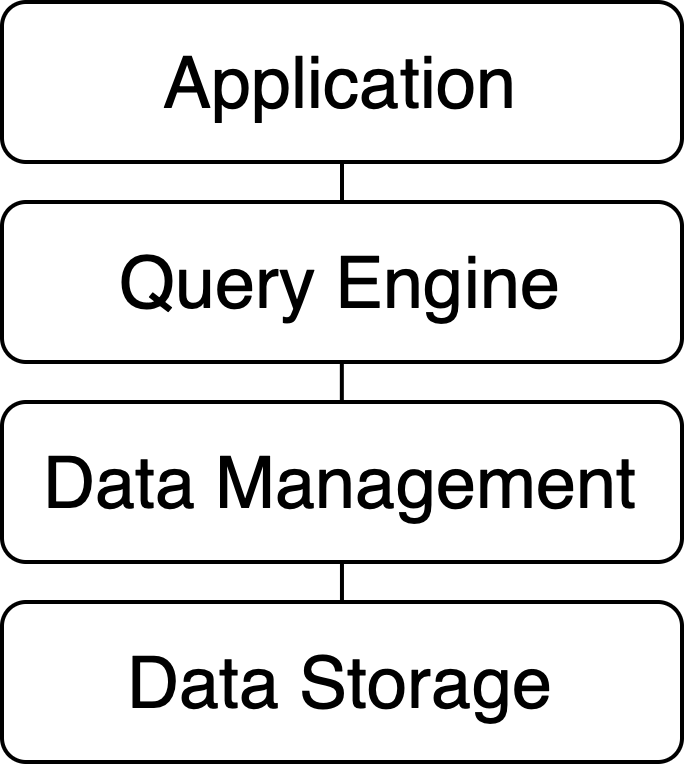
\includegraphics[width=0.4\textwidth]{figures/2-background/data_stack.png}
    \end{center}
    \caption{Data stack abstraction for this project}
    \label{fig:data_stack}
\end{figure}

The data stack (and this chapter) is divided into four sections:
\begin{enumerate}
    \item \textbf{Data Storage}: handles how the data is stored. The data storage layer might be centralized or distributed, on-premise or on the cloud, storing data in files, objects, or blocks.
    \item \textbf{Data Management} : handles how the data is managed. The data management layer might offer \gls{ACID} properties, data versioning, support open data formats, and/or support structured and/or unstructured data.
    \item \textbf{Query Engine}: handles how data is queried, i.e. accessed, retrieved and written. The query engine might offer caching, highly scalable architectures, and/or \gls{API} support for multiple programming languages.
    \item \textbf{Application}: a system that will take advantage of the data stack. In the case of this project, only the software of the host organization (Hopsworks' Feature Store) will be described. 
\end{enumerate}
After explaining the data stack, a section on programming languages complements the Background by explaining the roles different programming languages play in the data stack (namely, Python, Java, and Rust).


\section{Data storage}
    \label{sec:data_storage}
    This section aims to describe the data storage layer of this project, namely \gls{HopsFS}. \gls{HopsFS} is Hopsworks's evolution of \gls{HDFS}, a distributed file system. \gls{HopsFS} complexity will be broken down into parts, providing not only a great understanding of the tool, but also a comparison with common alternatives, namely cloud object stores.

\subsection{File storage vs. Object storage vs. Block storage}

Data can be stored and organized in physical storages, such as \glspl{HDD} and/or \glspl{SSD}, in three major ways: (1) Files, (2) Objects, (3) Blocks. For each one, the technique is briefly described and then a comparative table is showed (Table \ref{tab:storagecomparison}). This subsection is a rework according to the author's understanding of three articles coming from major cloud providers (Amazon, Google and IBM) \cite{BlockVsFile, HowObjectVs, ObjectVsFile2021}.

\subsubsection*{File storage}

File storage is a hierarchical data storage technique that stores data into files. A file is a collection of data characterized by an file extension (e.g. ".txt", ".png", ".csv", ".parquet") that indicates how the data contained is organized. Every file is contained within a directory, that can contain other files or other directories (called "subdirectories"). In many file storages directories are called "folders". 

This type of structure, very common in modern \glspl{PC}, simplifies locating and retrieving a single file and its flexibility allows it to store any type of data. However, its hierarchical structure requires that to access a file, its exact location should be known. This restriction decreases the scaling possibilities of the system, where a large amount of data needs to be retrieved at the same time.

Overall, this solution is still vastly popular in user-facing storage applications (e.g. Dropbox, Google Drive, One Drive) and \glspl{PC} thanks to its intuitive structure and ease of use. On the other hand, other options are preferred for managing large quantities of data, due to its lacks in scalability. \\[3mm]
\noindent\textbf{Advantages}
\begin{itemize}
    \item Ideal for small-scale operations (low latency, efficient folderization).
    \item User familiarity and ease of management.
    \item File-level access permissions and locking capabilities.
\end{itemize}

\noindent\textbf{Disadvantages}
\begin{itemize}
    \item Difficult to scale due to deep folderization.
    \item Inefficient in storing unstructured data.
    \item Limitations in scalability due to reaching device or network capacity.
\end{itemize}

\subsubsection*{Object storage}

Object storage is a flat data storage technique that stores data into objects. An object is an isolated container associated with metadata, i.e. a set of attributes that describe the data e.g. a unique identifier, object name, size, creation date. Metadata is used to retrieve the data more easily, allowing for queries that retrieve large quantities of data simultaneously, e.g. all data that was created on a specific date. 

The flat structure of Object storage, where all objects are in the same container called bucket, is ideal for managing large quantities of unstructured data (e.g. videos, images). This structure is also easier to scale as it can be replicated easily across multiple regions allowing an faster access in different areas of the world, and fault tolerance to hardware failure.

On the other hand, objects cannot be altered once created, and in case of a change must recreated. Also, object stores are not ideal for transactional operations as objects cannot have a locking mechanism. Lastly, object stores have slower writing performance compared to file or block storage solutions.

Overall, this solution is widely when high scalability is required (e.g. social networks, video streaming apps) thanks to its flat structure and use of metadata. On the other hand, other options are preferred when transactional operations are required, or high performance on a small number of files that change frequently are necessary. \\[3mm]
\noindent\textbf{Advantages}
\begin{itemize}
    \item Potential unlimited scalability.
    \item Effective use of metadata enabling advanced queries.
    \item Cost-efficient storage for all types of data (also unstructured).
\end{itemize}

\noindent\textbf{Disadvantages}
\begin{itemize}
    \item Absence of file locking mechanisms.
    \item Low performance (increased latency and processing overhead).
    \item Lacks data update capabilities (only recreation).
\end{itemize}

\subsubsection*{Block storage}

Block storage is a data storage technique that divides data into blocks of fixed size that can be read or written individually. Each block is associated to a unique identifier and it is then stored on a physical server (note that a block can be stored in different \glspl{OS}). When the user requests the data saved, the block storage retrieves the data from the associated blocks and then re-assembles the data of the blocks into a single unit. The block storage also manages the physical location of the block, saving a block where is more efficient.

Block storage is very effective for systems needing fast access and low latency. This architecture is compatible with frequent changes, unlike object storage.

On the other hand, block storage achieves its speed operating at a low level on physical systems, so the cost of the architecture is strictly bound on the storage and servers used, not allowing to scale the architecture on the demands needs. \\[3mm]
\noindent\textbf{Advantages}
\begin{itemize}
    \item High performance (low latency).
    \item Reliable self-contained storage units.
    \item Data stored can be modified easily.
\end{itemize}

\noindent\textbf{Disadvantages}
\begin{itemize}
    \item Lack of metadata brings limitations in data searchability.
    \item High cost to scale the infrastructure.
\end{itemize}

\begin{table}[!ht]
    \begin{center}
      \caption{Comparison between data storage different characteristics.}
      \label{tab:storagecomparison}
      \begin{tabular}{cccc} % <-- Alignments: 1st column left, 2nd middle, with vertical lines in between
        \toprule
        \textbf{Characteristics}\Tstrut\Bstrut & \textbf{File Storage} & \textbf{Object Storage} & \textbf{Block Storage}\\
        \midrule
        Performance & High & Low & High\Tstrut\\
        Scalability & Low & High & Low\\
        Cost & High & Low & High\Bstrut\\
        \bottomrule
      \end{tabular}
    \end{center}
\end{table}

\subsection{\glsfmtlong{HDFS}}

\glsentryfull{HDFS} is a \gls{DFS}, i.e. a file system that uses distributed storage resources while providing a single namespace as a traditional file system. \gls{HDFS} has significant differences compared with other \glspl{DFS}.\gls{HDFS} is highly fault-tolerant, i.e. it is resistent to hardware failures of part of its infrastructure, and can be deployed on commodity hardware. \gls{HDFS} also provides high throughput access to application data and it is designed to be highly compatible with applications with large datasets (more than 100 GB) \cite{borthakurHadoopDistributedFile2005}. 

\gls{HDFS} architecture consists of a single primary node called Namenode and multiple secondary nodes called Datanodes. The Namenode manages the filesystem namespace and regulates access to files by clients. On the other hand, Datanodes manage the storage attached to the nodes they run on and they are responsible for performing replication requests when prompted by the Namenode. \gls{HDFS} exposes to users a file system namespace where data can be stored in files. Internally, a file is divided into one or multiple blocks and these blocks are store in a set of Datanodes. The blocks are also replicated upon the first write operation, up to a certain number of times (by default three times, with at least one copy on a different physical infrastructure). The Namenode keeps track of the data location, matching it with the filesystem namespace. It is also responsible for managing Datanode reachability (through periodical state messages sent by Datanodes), and providing clients with the locations of the Datanodes containing the blocks that compose the requested file. If a new write request is received, it is still the Namenode that needs to provide the locations of available storage for the file blocks. 

In Figure \ref{fig:hdfs} a simplified visual representation of the Namenode and Datanodes basic operations in \gls{HDFS} is present.

\begin{figure}[!ht]
    \begin{center}
      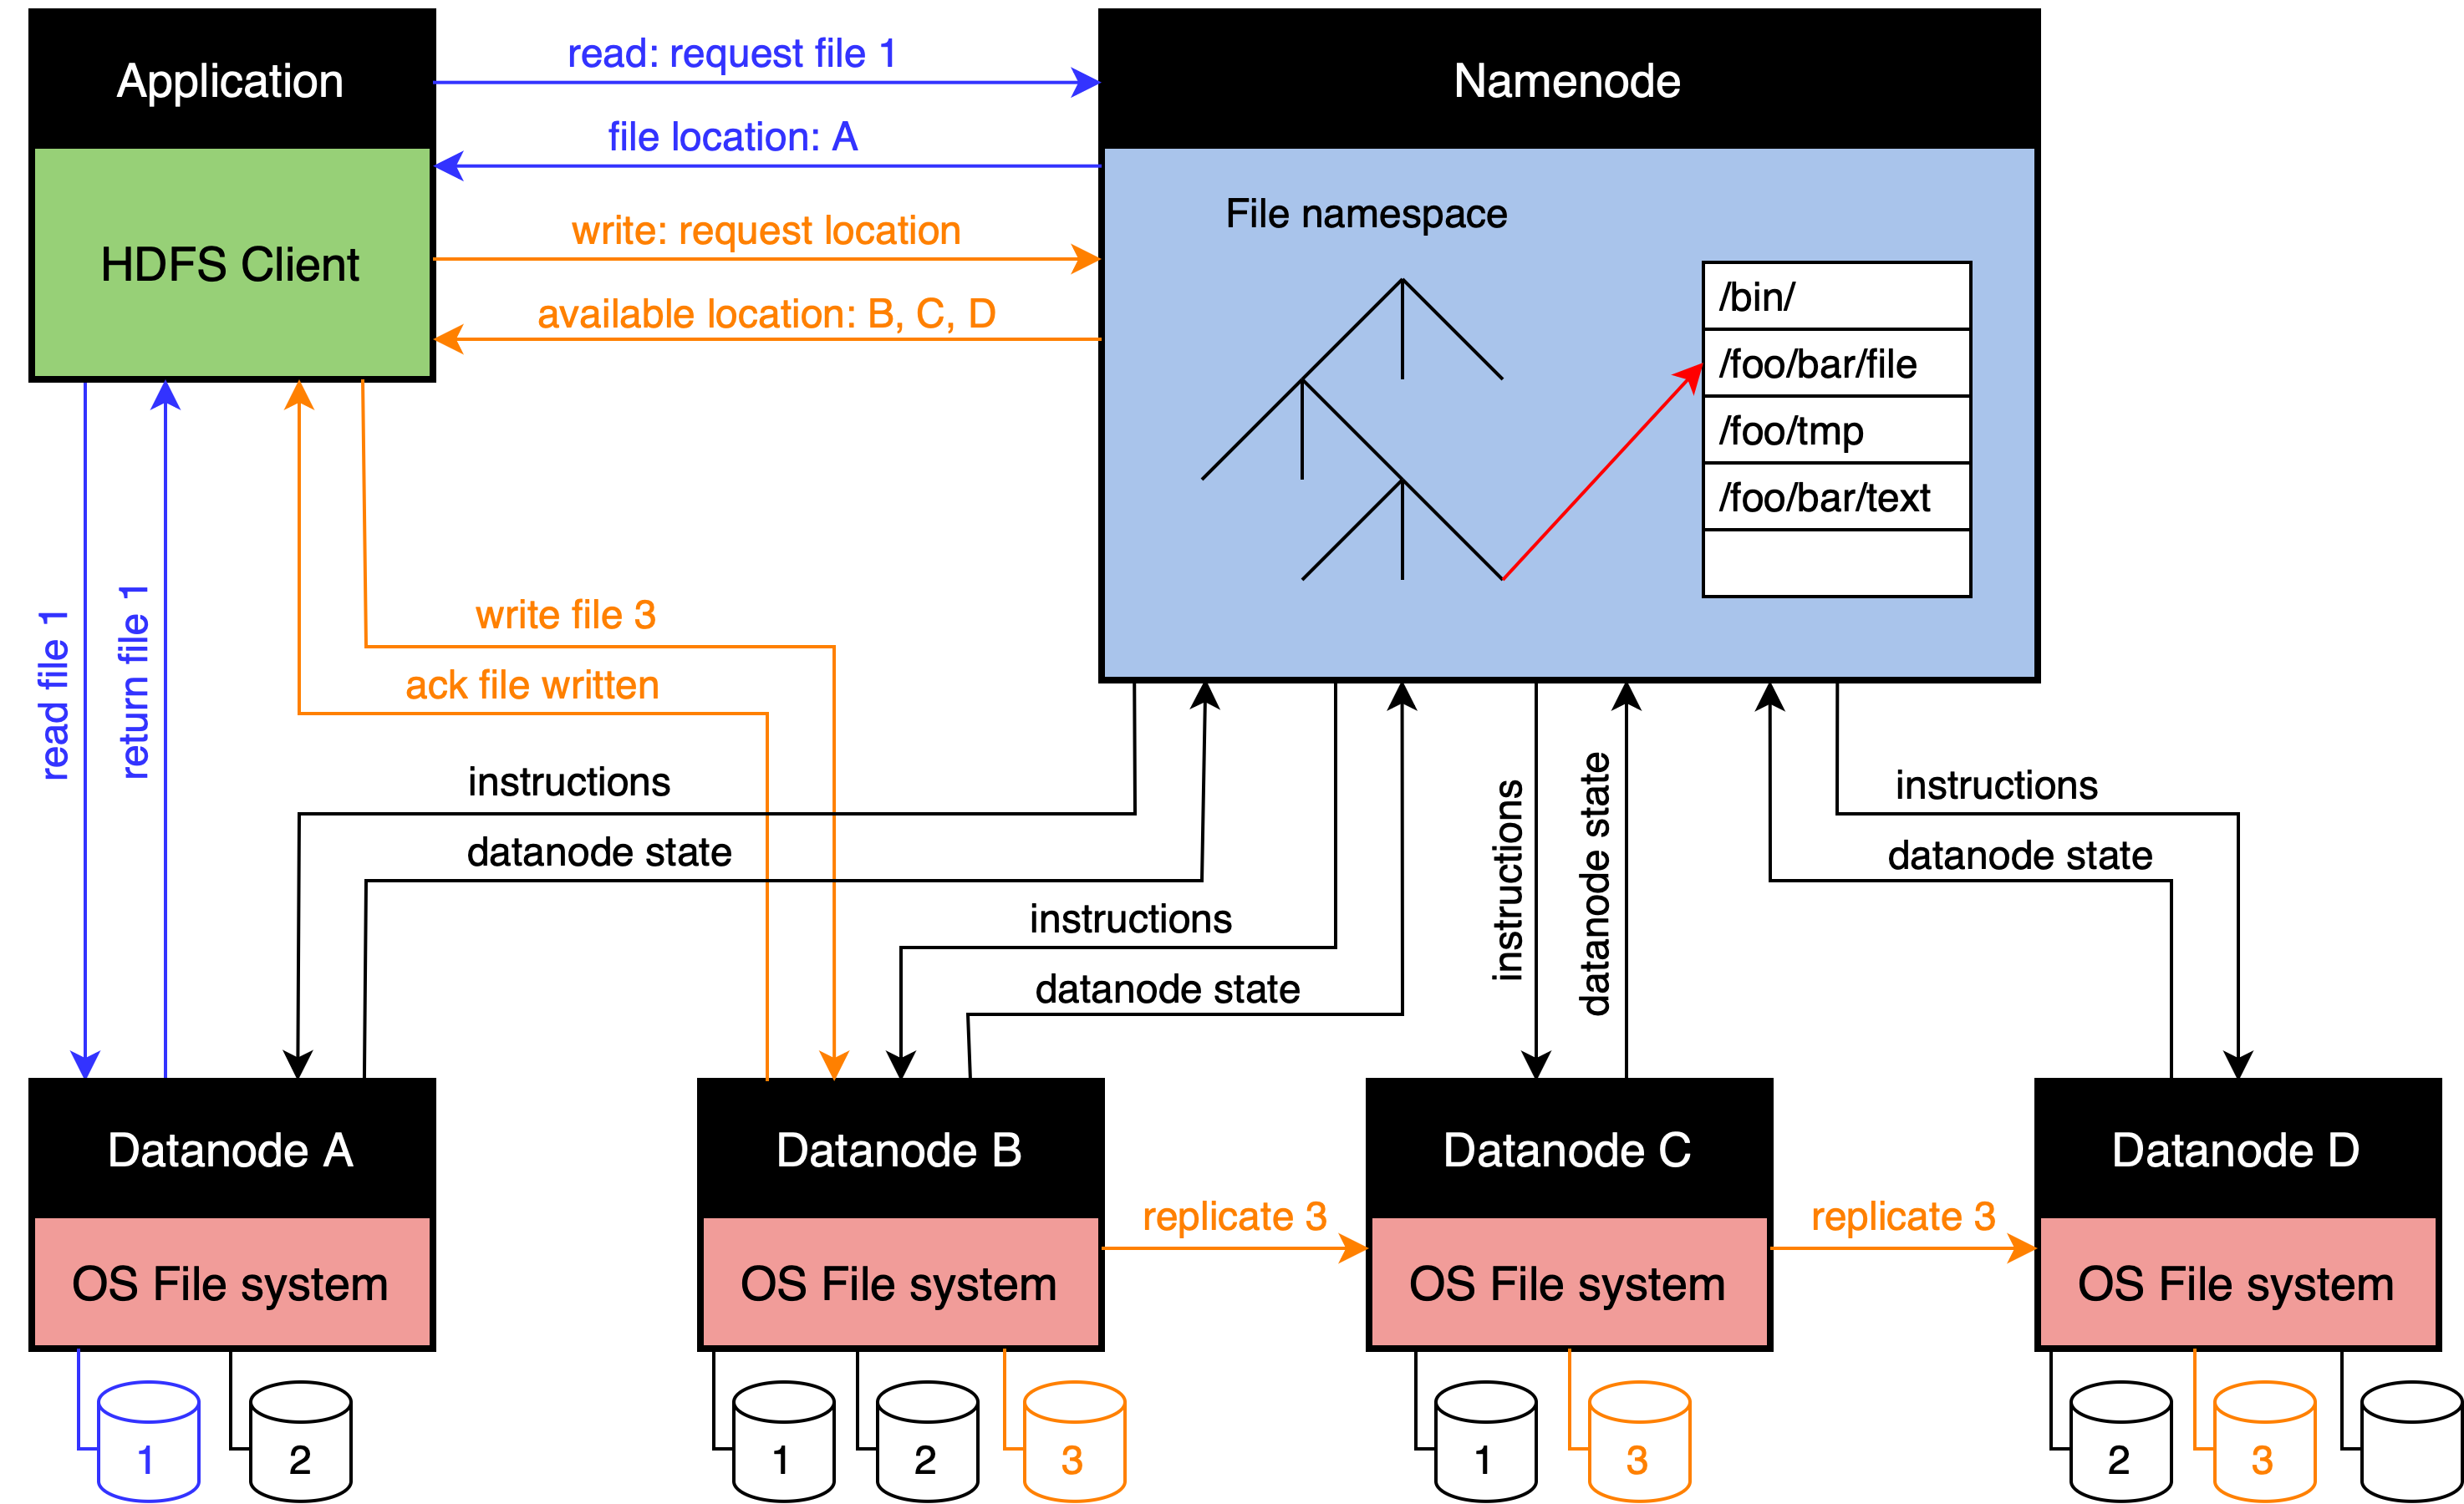
\includegraphics[width=\textwidth]{figures/2-background/HDFS.png}
    \end{center}
    \caption{\glsentryfull{HDFS} architecture displaying in different colors basic operations: read (blue), write (orange) and Namenode-Datanodes management messages (black). Note: for representation simplicity files are not segmented into blocks.}
    \label{fig:hdfs}
\end{figure}
 
\subsection{\gls{HopsFS} as an \glsfmtshort{HDFS} evolution}



\subsection{\glsfmtshort{HDFS} alternatives: Cloud object stores}

\section{Data management}
    \label{sec:data_management}
    % Intro on the section
This section describes the data management layer for this project, i.e. how data is managed, versioned, etc. The main \gls{DBMS} technology used in this is Delta Lake, and to understand it Section \ref{subsec:history_DBMS} revises the problems that technologies aimed to solve, and the limitations of these systems. The chapter is complemented with Section \ref{subsec:delta_lake_access} which explains how to access Delta Lake and introduces delta-rs.

\subsection{Brief history of \glsfmtlongpl{DBMS}}
\label{subsec:history_DBMS}

In recent years the rise of Big Data, large volumes of various structured and unstructured data types at a high velocity, has shown an incredible potential but it has also posed several challenges \cite{penceWhatBigData2014}. These mostly impact the software architecture that needs to deal with these issues, which led to an evolution of these technologies \cite{gortonDistributionDataDeployment2015}. Delta Lake \cite{armbrustDeltaLakeHighperformance2020}, is one of the most recent iterations of this evolution process, but to understand the tool, it is necessary to understand the challenges, starting from the beginning of the data management evolution.

Before Big Data, companies already wanted to gain insights from their data sources using an automated workflow. Here is where \gls{ETL} and relational databases first came into use. An \gls{ETL} pipeline as the name suggests:
\begin{enumerate}
    \item Extracts data from \glspl{API} or other company's data sources.
    \item Transforms data by removing errors or absent fields, standardizes the format to match the database, and validates the data to verify its correctness.
    \item Loads it into a relational database (e.g. MySQL).
\end{enumerate} 

\begin{figure}[!ht]
    \begin{center}
      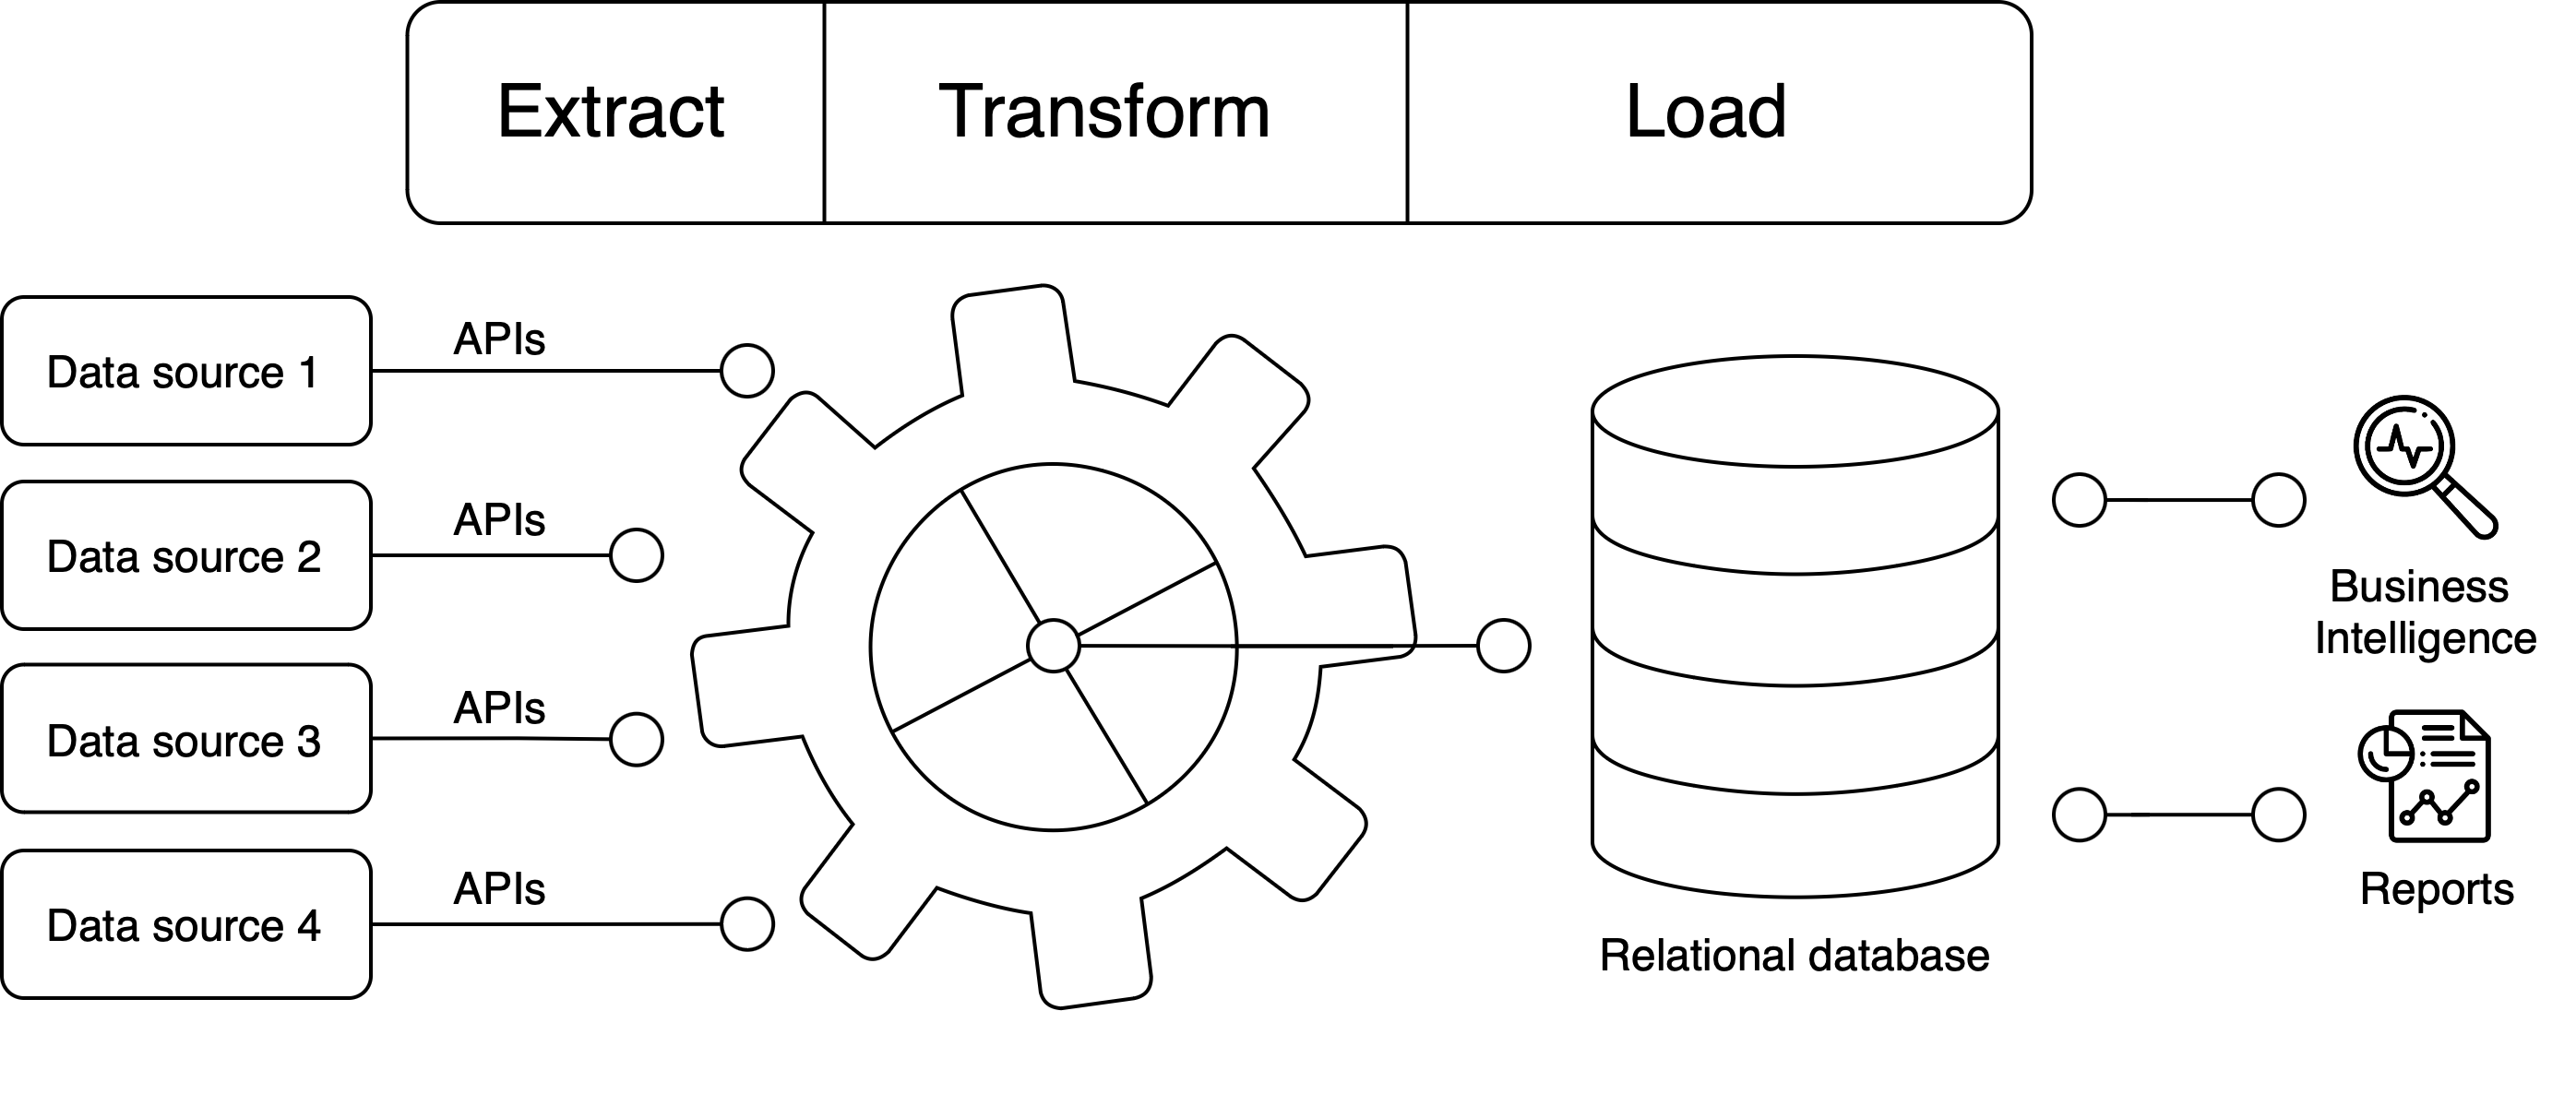
\includegraphics[width=\textwidth]{figures/2-background/DeltaLake_evolution-ETL+DB.png}
    \end{center}
    \caption[ETL system with a relational database]{\gls{ETL} system with a relational database. Diagram inspired by AltexSoft educational video available at \url{https://www.youtube.com/watch?v=qWru-b6m030}.}
    \label{fig:ETL+DB}
\end{figure}
% Figure inspired by AltexSoft video \cite{altexsoftHowDataEngineering2021}

This type of workflow, represented in Figure \ref{fig:ETL+DB}, enabled companies to obtain \gls{BI} insights and data reports on the company's data. The main limitation of this system sat in its limited capability of creating reports or \gls{BI} insights based on data sitting on multiple tables. These types of requests are called analytical queries, and while they might run less often than simpler queries are still crucial for making data-driven decisions (e.g. determining the region that sold more product units in the last year).

When the need to compute analytical queries rose, more complex \gls{DBMS} substituted the simple relational databases, optimizing for running business-centric complex analytical queries. These systems are called \gls{OLAP}, and its prime example example is the data warehouse.

\begin{figure}[!ht]
    \begin{center}
      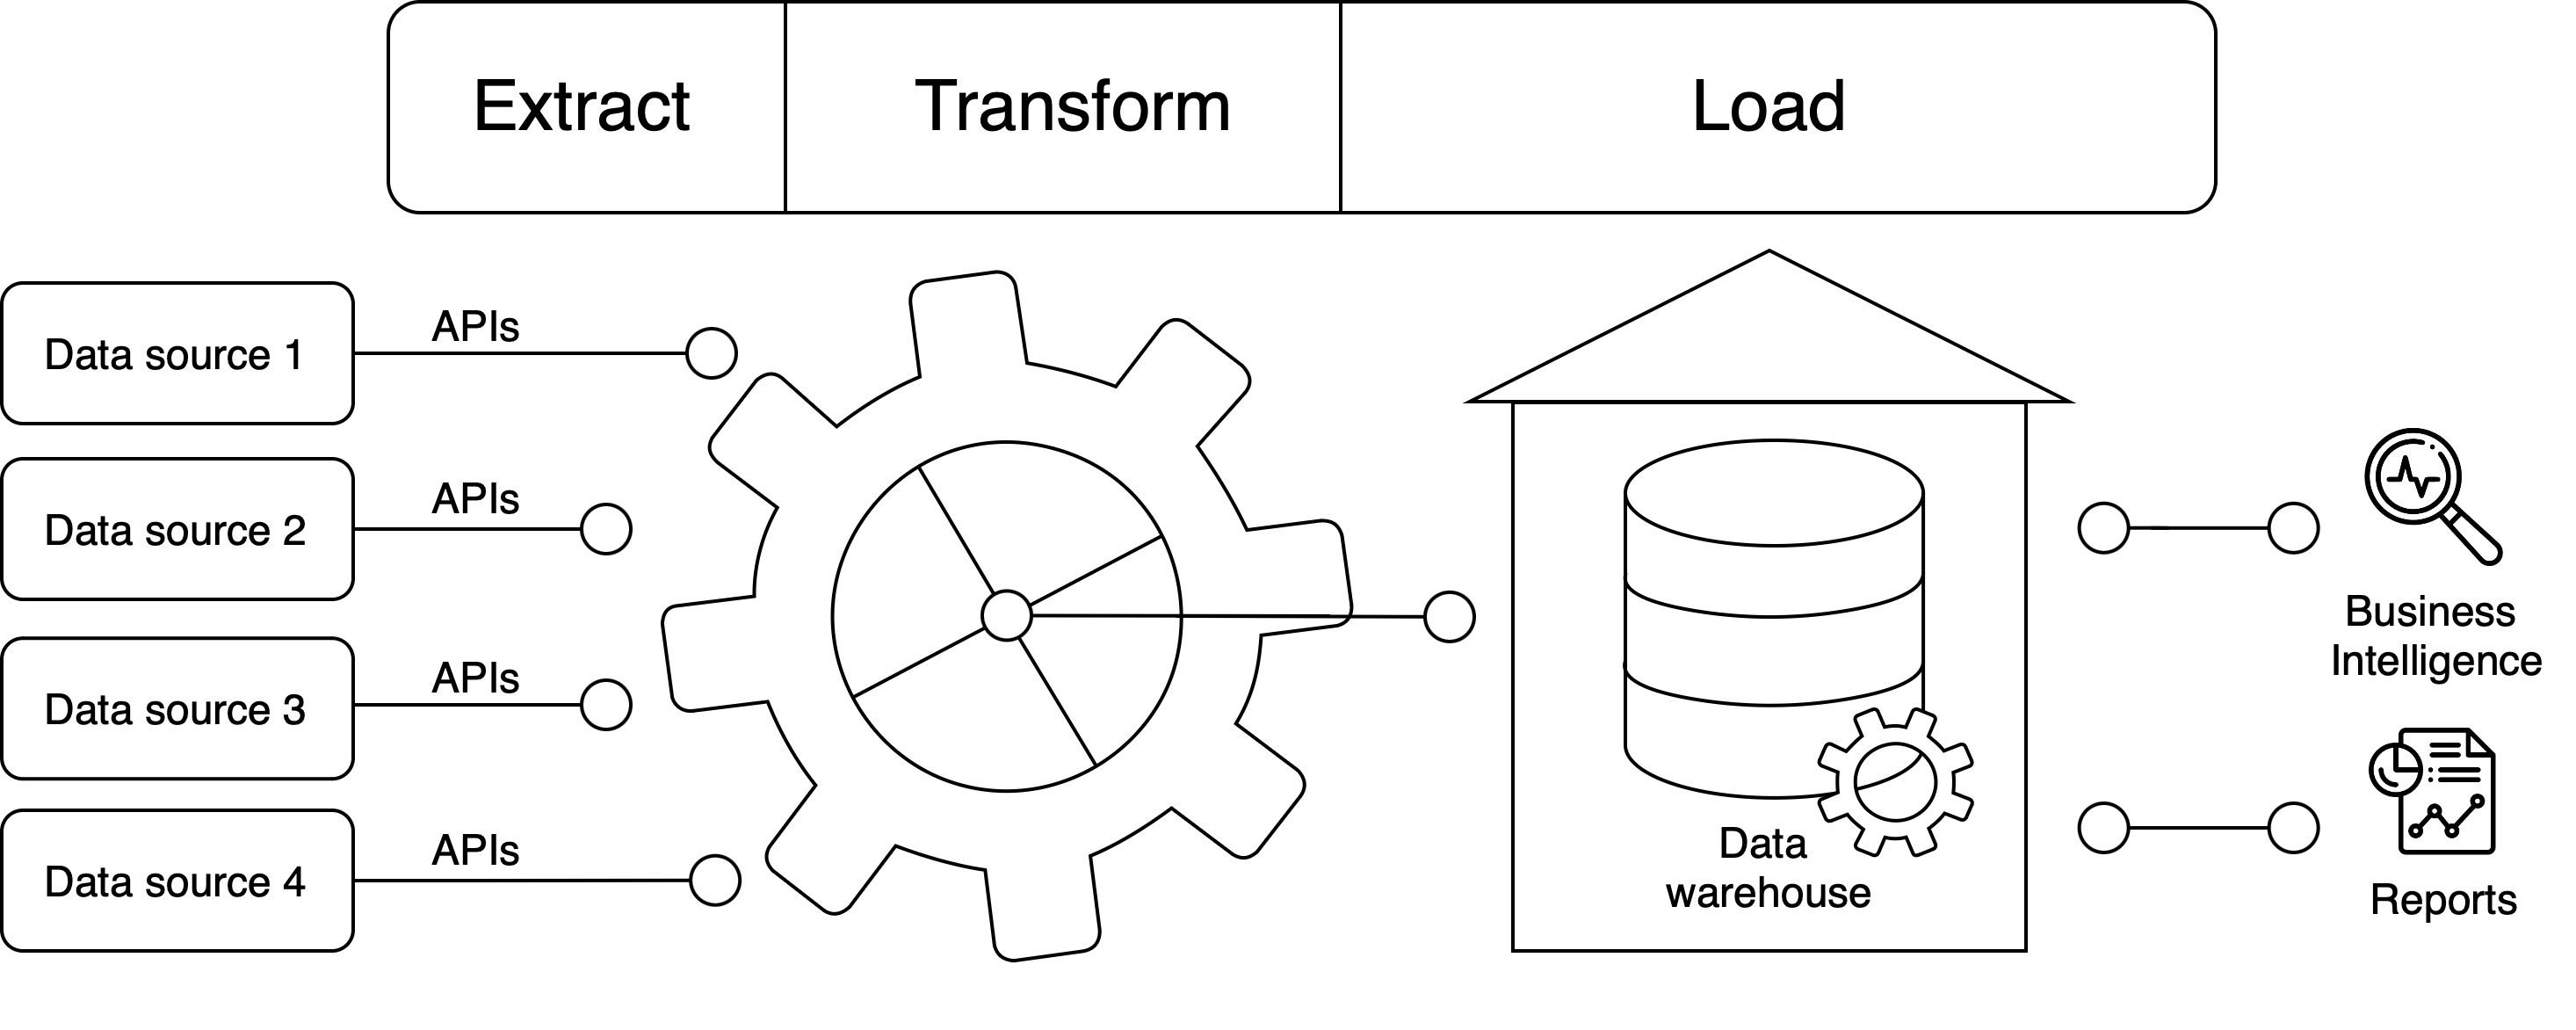
\includegraphics[width=\textwidth]{figures/2-background/DeltaLake_evolution-ETL+DW.png}
    \end{center}
    \caption[ETL system with a data warehouse]{\gls{ETL} system with a data warehouse. Diagram inspired by AltexSoft educational video available at \url{https://www.youtube.com/watch?v=qWru-b6m030}.}
    \label{fig:ETL+DW}
\end{figure}

A data warehouse workflow, visualized in Figure \ref{fig:ETL+DW}, enables larger quantities of data to be computed and analyzed. Data warehouses enable \gls{BI} and Reports that consider all data sources and can join multiple tables efficiently. This type of \gls{DBMS} still keeps a relational database key features, such as \gls{ACID} transactions and data versioning.

Over time, the rapidly growing amount of unstructured data (also called Big Data, e.g. images, and videos) created new needs within companies, that wanted to take advantage of this new data. Data warehouses were unfit to solve this problem as they only supported structured data. Furthermore, storing large quantities of data in data warehouses is expensive and does not support any type of \gls{AI}/\gls{ML} workflow.

These issues were tackled by a new paradigm called Data Lake (Figure \ref{fig:ELT+DL}). Data Lakes are based on a low-cost object storage system (Section \ref{subsec:file_vs_obj_vs_block}) that consists of a flat structure where all data is loaded after extraction. In data lakes the architecture structure changes as data is first loaded into the data lake and only after transformed. This paradigm is called \gls{ELT}. Transformations are customizable for specific applications, e.g. \gls{BI} and reports using a Data warehouse, an \gls{AI}/\gls{ML} analysis.

\begin{figure}[!ht]
    \begin{center}
      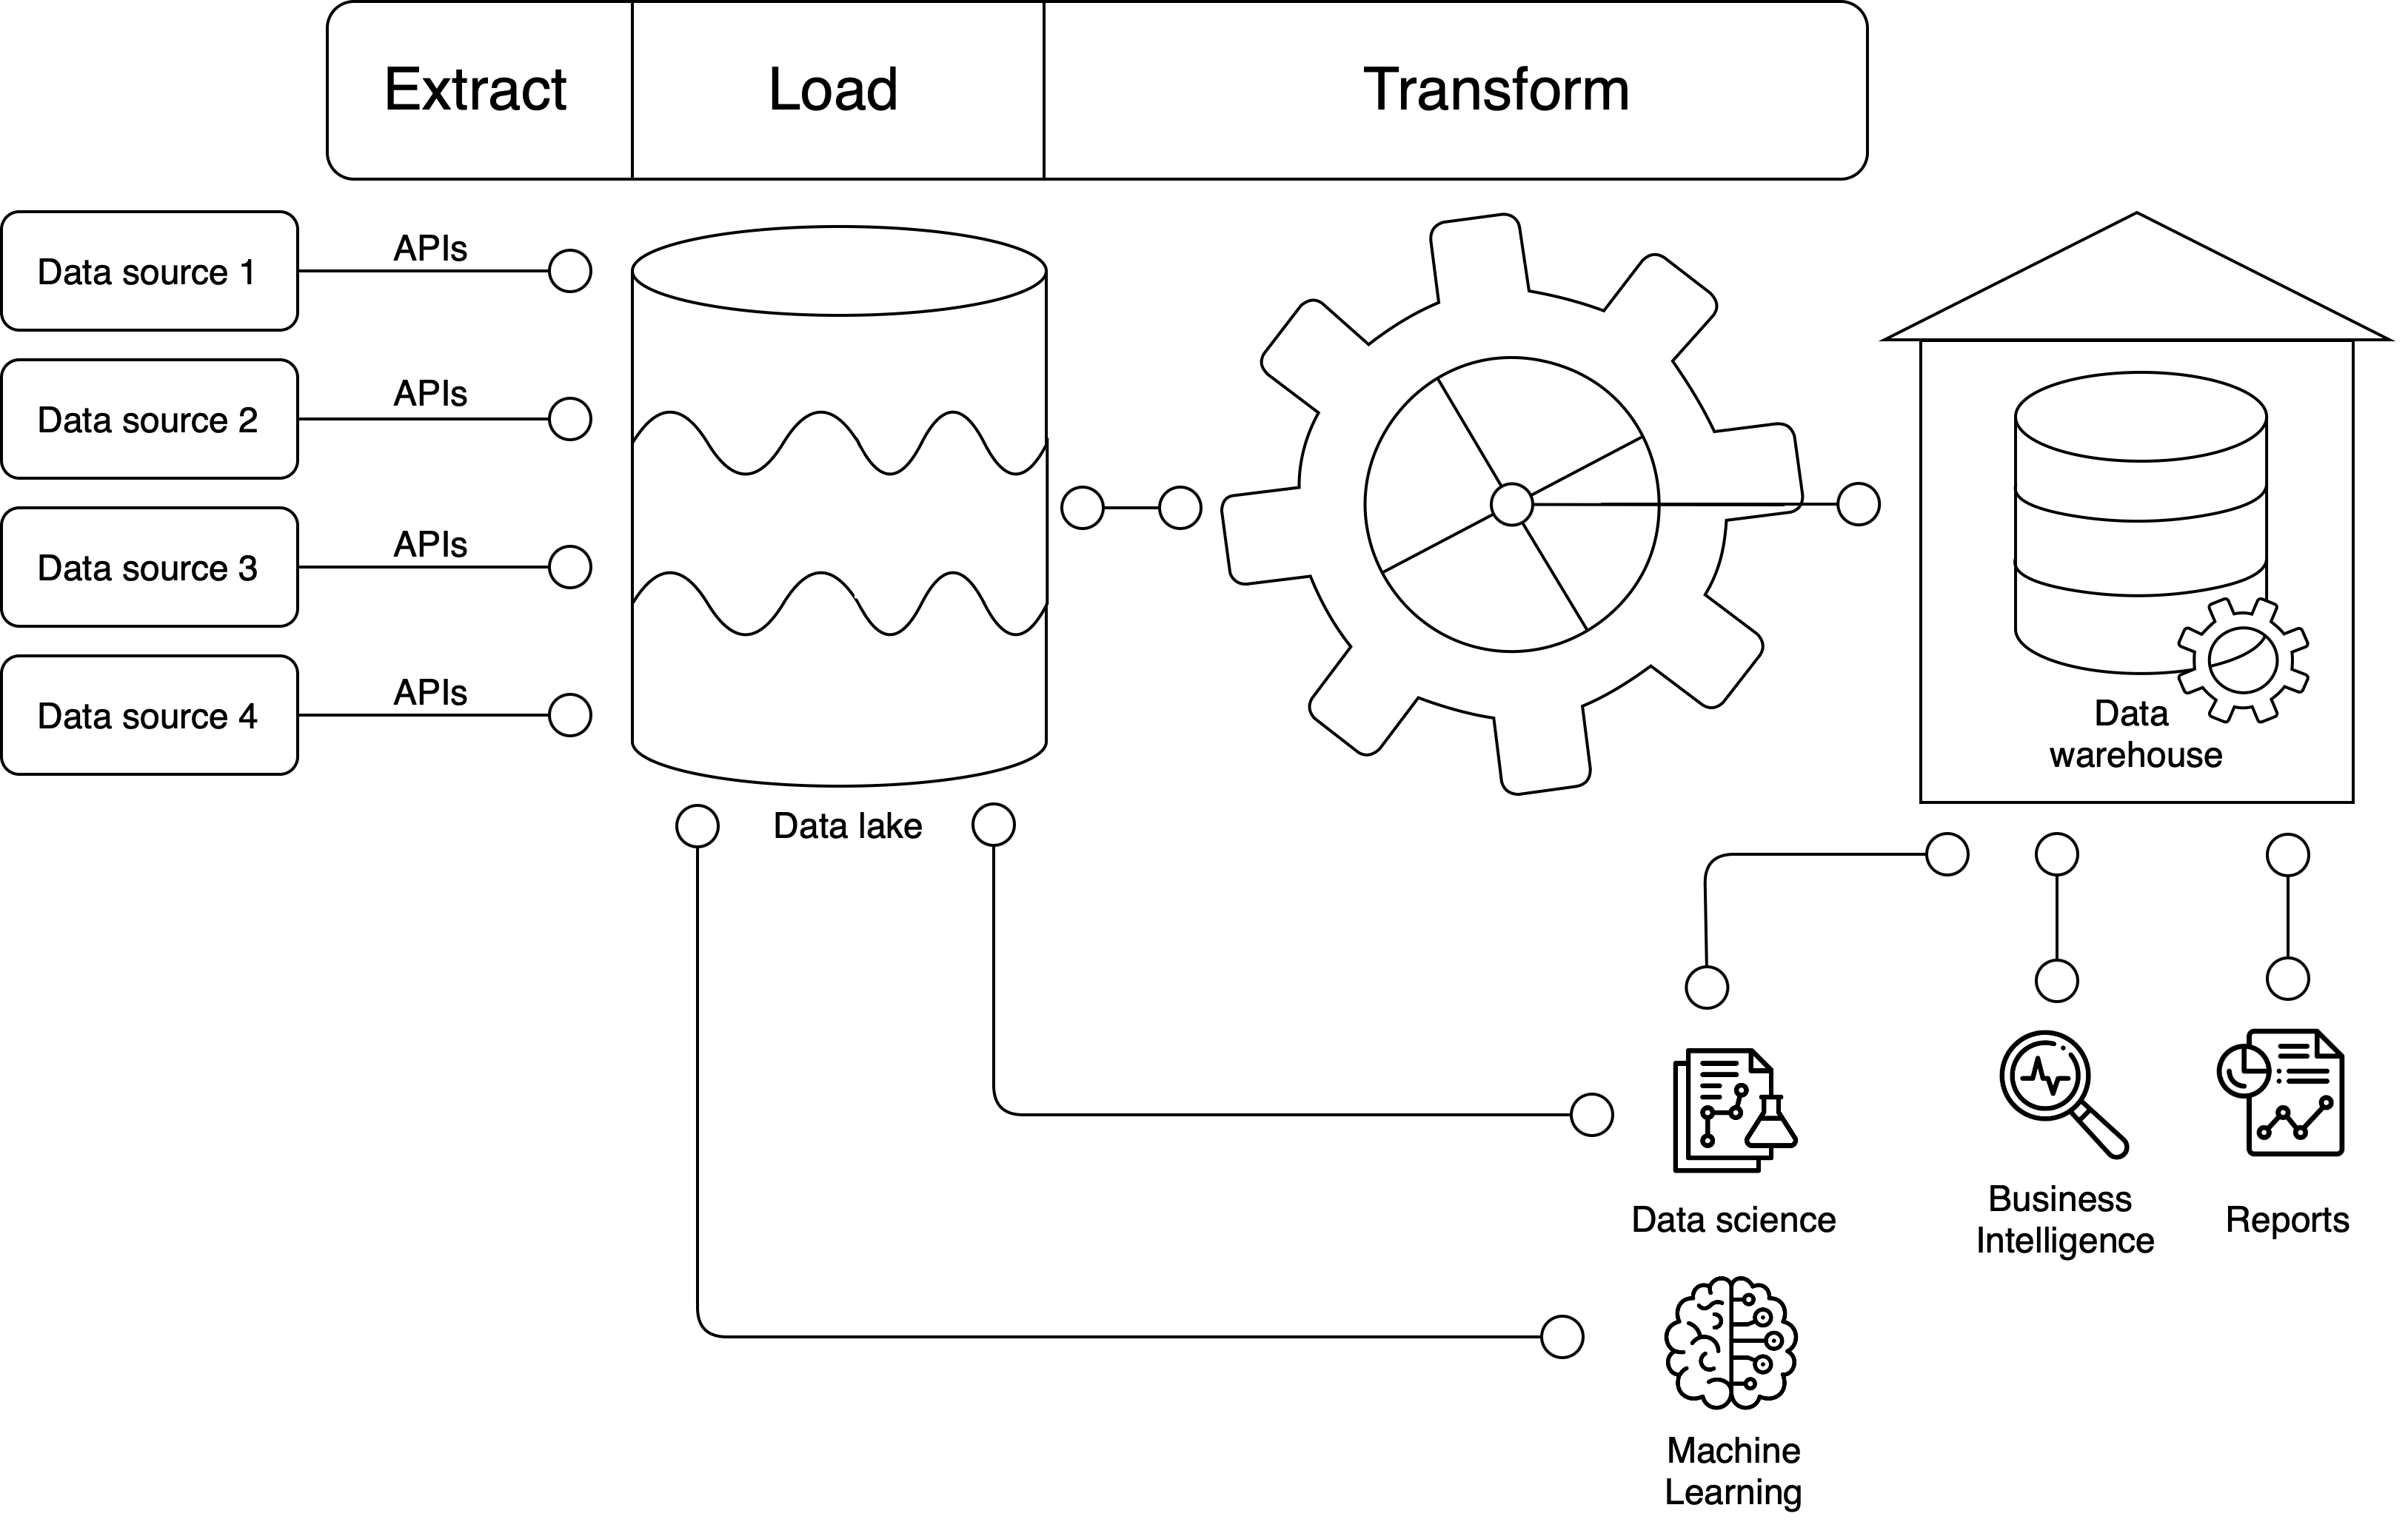
\includegraphics[width=\textwidth]{figures/2-background/DeltaLake_evolution-ELT+DL.png}
    \end{center}
    \caption[ELT system with a data lake]{\gls{ELT} system with a data lake. Diagram inspired by AltexSoft educational video available at \url{https://www.youtube.com/watch?v=qWru-b6m030}.}
    \label{fig:ELT+DL}
\end{figure}

This architecture reduces storage costs but also increases the system complexity. Higher complexity is typically related to higher costs, as system maintenance is more costly and can lead to a larger number of issues. Additionally, since data lake cannot be queried directly with \gls{BI} queries or requesting business reports, this leads to the need to still maintain a data warehouse (as in Figure \ref{fig:ELT+DL}). This ultimately leads to higher costs to maintain the multiple storages for the same data. The system also suffers from timeliness due to this lengthy pipeline, as the data needs to go through many steps before it is available in the data warehouse. 

These issues outlined that data lakes were not a drop-in replacement for data warehouses, as they served a different purpose and suffered from different issues. This generated the need to have a system that could have data warehouses \gls{ACID} and data management capabilities while being able to support unstructured data. The solution was a new architecture, the data lakehouse. 

\begin{figure}[!ht]
    \begin{center}
      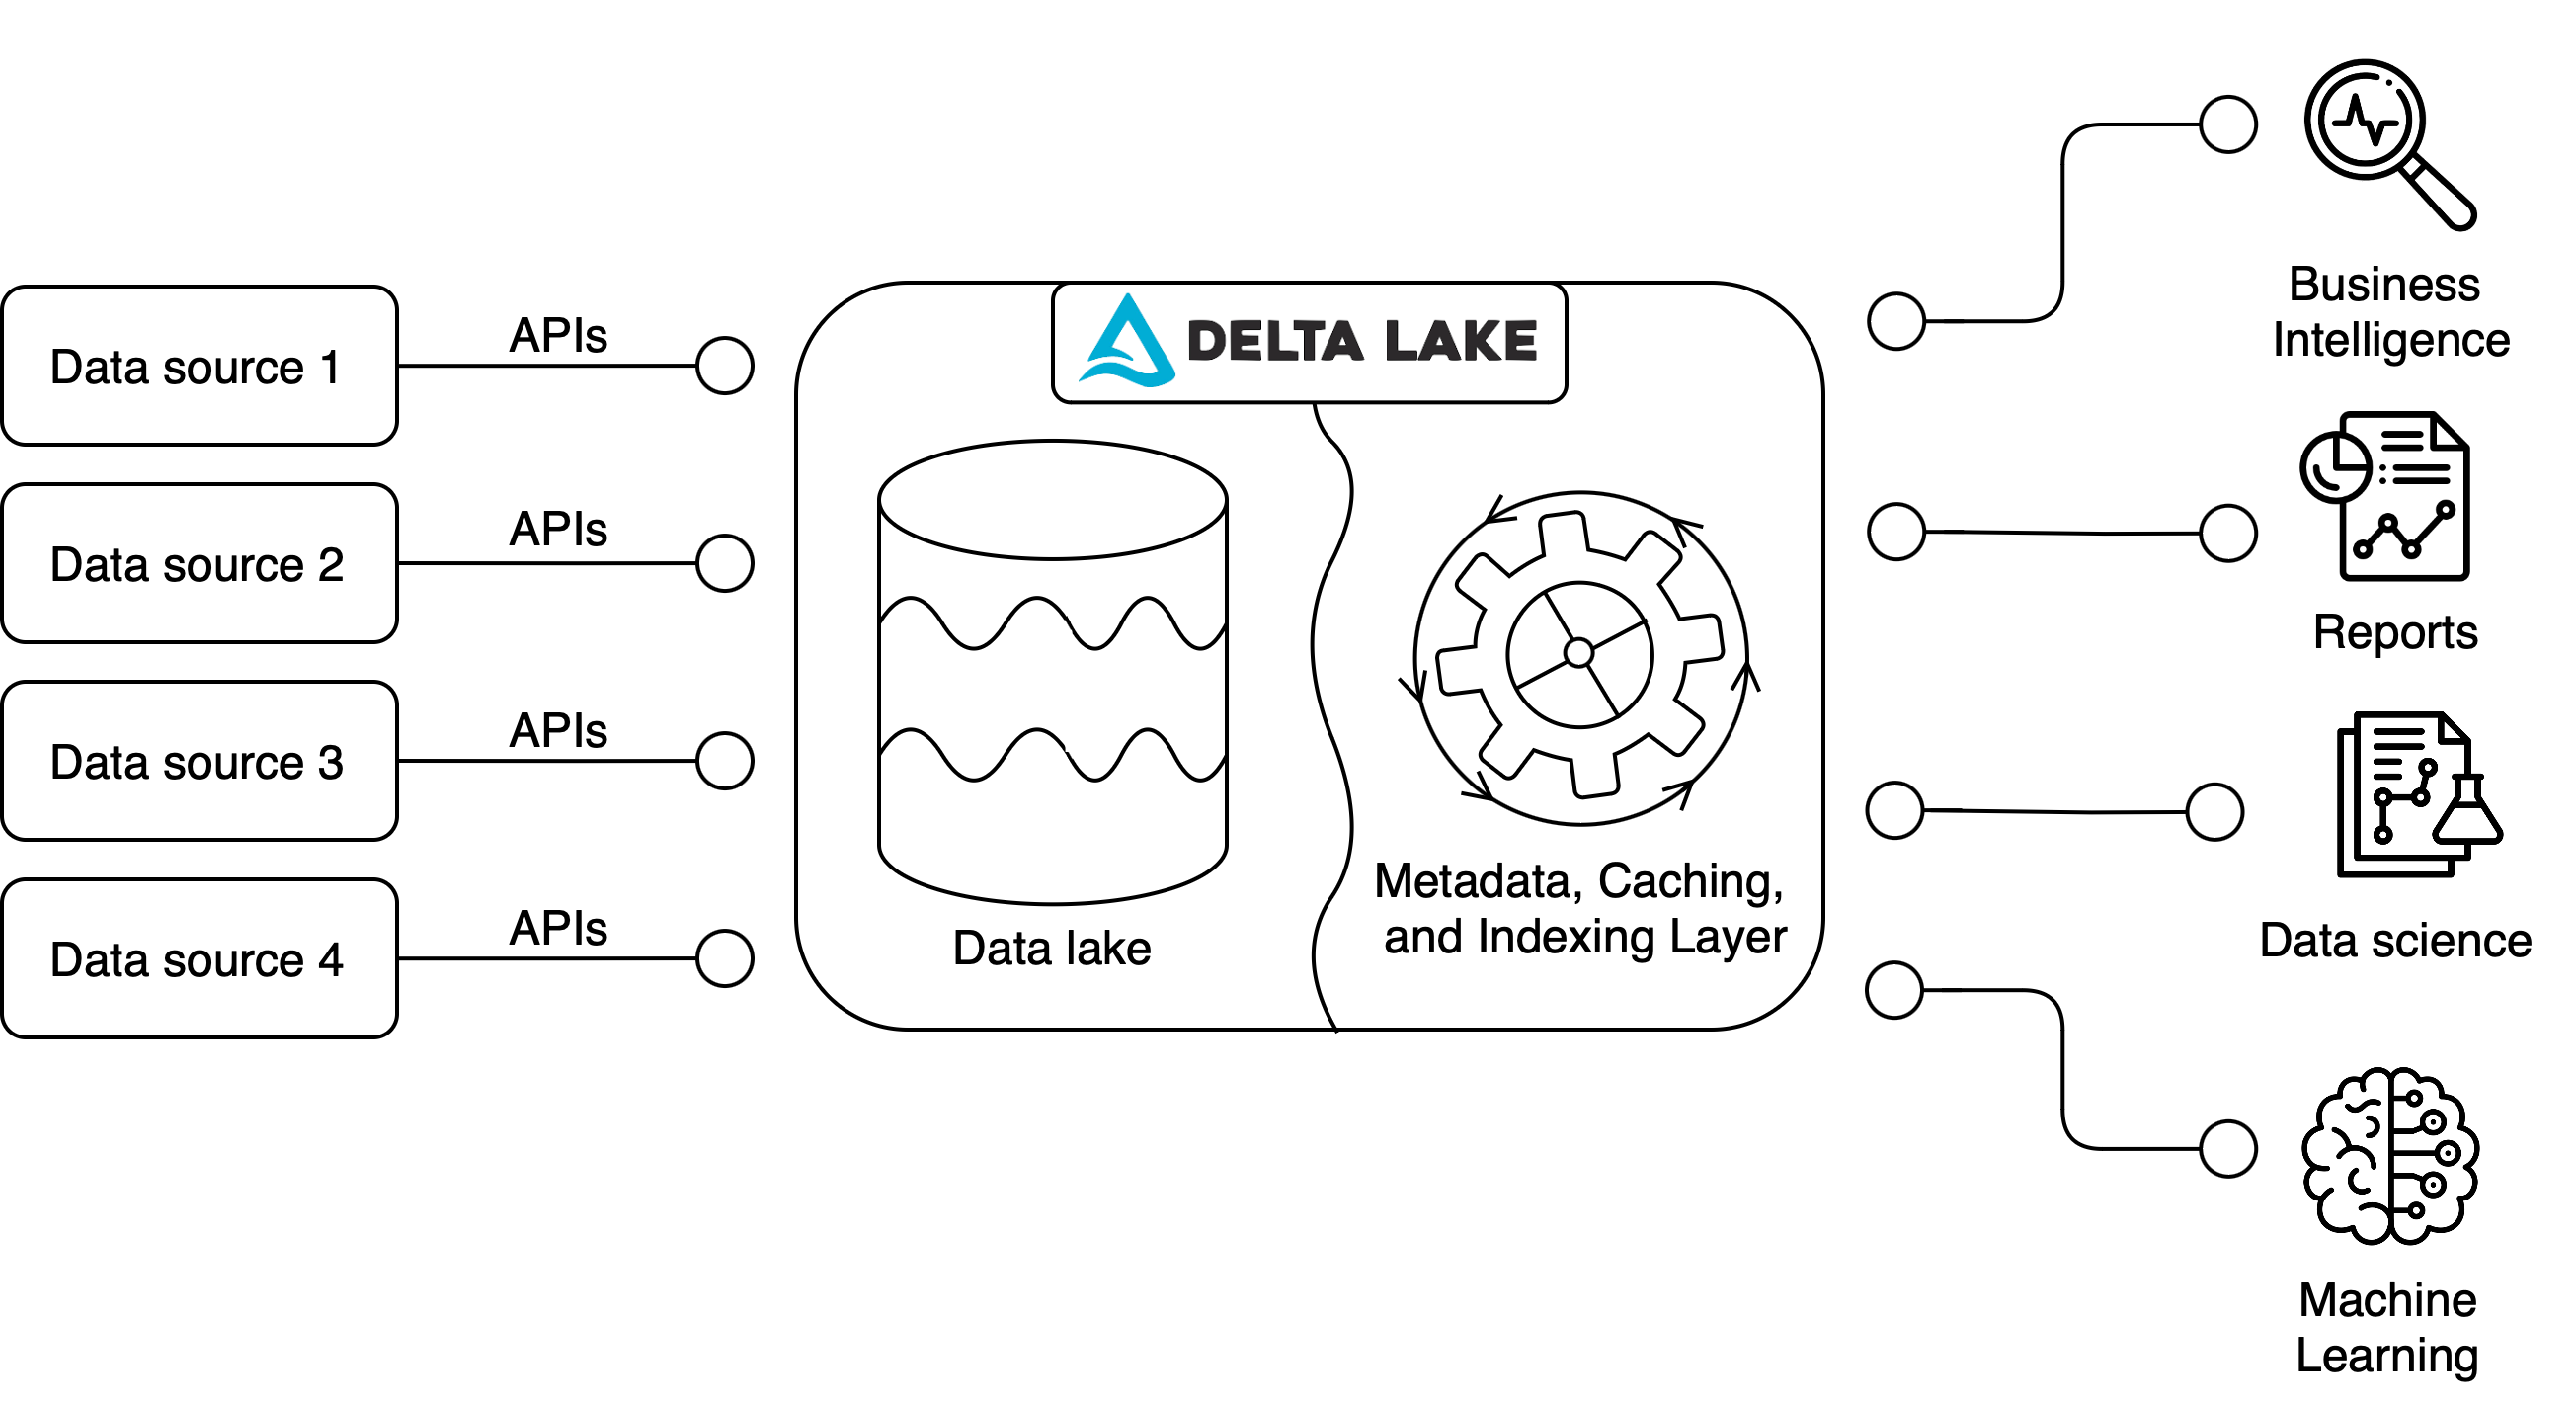
\includegraphics[width=\textwidth]{figures/2-background/DeltaLake_evolution-DeltaLake.png}
    \end{center}
    \caption[Delta lake architecture]{Delta lake architecture. Diagram inspired by Delta Lake paper \cite{armbrustDeltaLakeHighperformance2020}.}
    \label{fig:DeltaLake}
\end{figure}

Figure \ref{fig:DeltaLake} shows a Delta Lake system \cite{armbrustDeltaLakeHighperformance2020}. The data lakehouse term was first introduced by Databricks in 2021 with their paper presented at \gls{CIDR} \cite{lakehouse2021}, while data lakehouse solutions already existed on the market, namely Apache Hudi \cite{rajaperumalUberEngineeringIncremental2017}, Apache Iceberg and Delta Lake \cite{armbrustDeltaLakeHighperformance2020}. Data lakehouses combine the benefits of data warehouses and data lakes while simplifying the complexity of storing and accessing data in enterprise data architectures. This new architecture is based on an open-data format called Apache Parquet (from now on simply parquet), which is a column-based data file format. Data is saved in a data lake in the form of parquet files, then a management layer enables managing transactions, versioning, indexing, and other data management features. This enables data lakehouses to offer \gls{ACID} properties, similarly to data warehouses. 

Delta Lake is the technology that will be most used in this project. A Delta Lake Table (i.e. an instance of Delta Lake) works operating on a data lake containing parquet files and a transaction log. The transaction log records each operation, enabling versioning and recovery of previous versions (also called time travel). The data lake can be partitioned, e.g. using a date field, and this would make the Delta Lake table look as Figure \ref{fig:delta_table}. 

\begin{figure}
    \begin{center}
      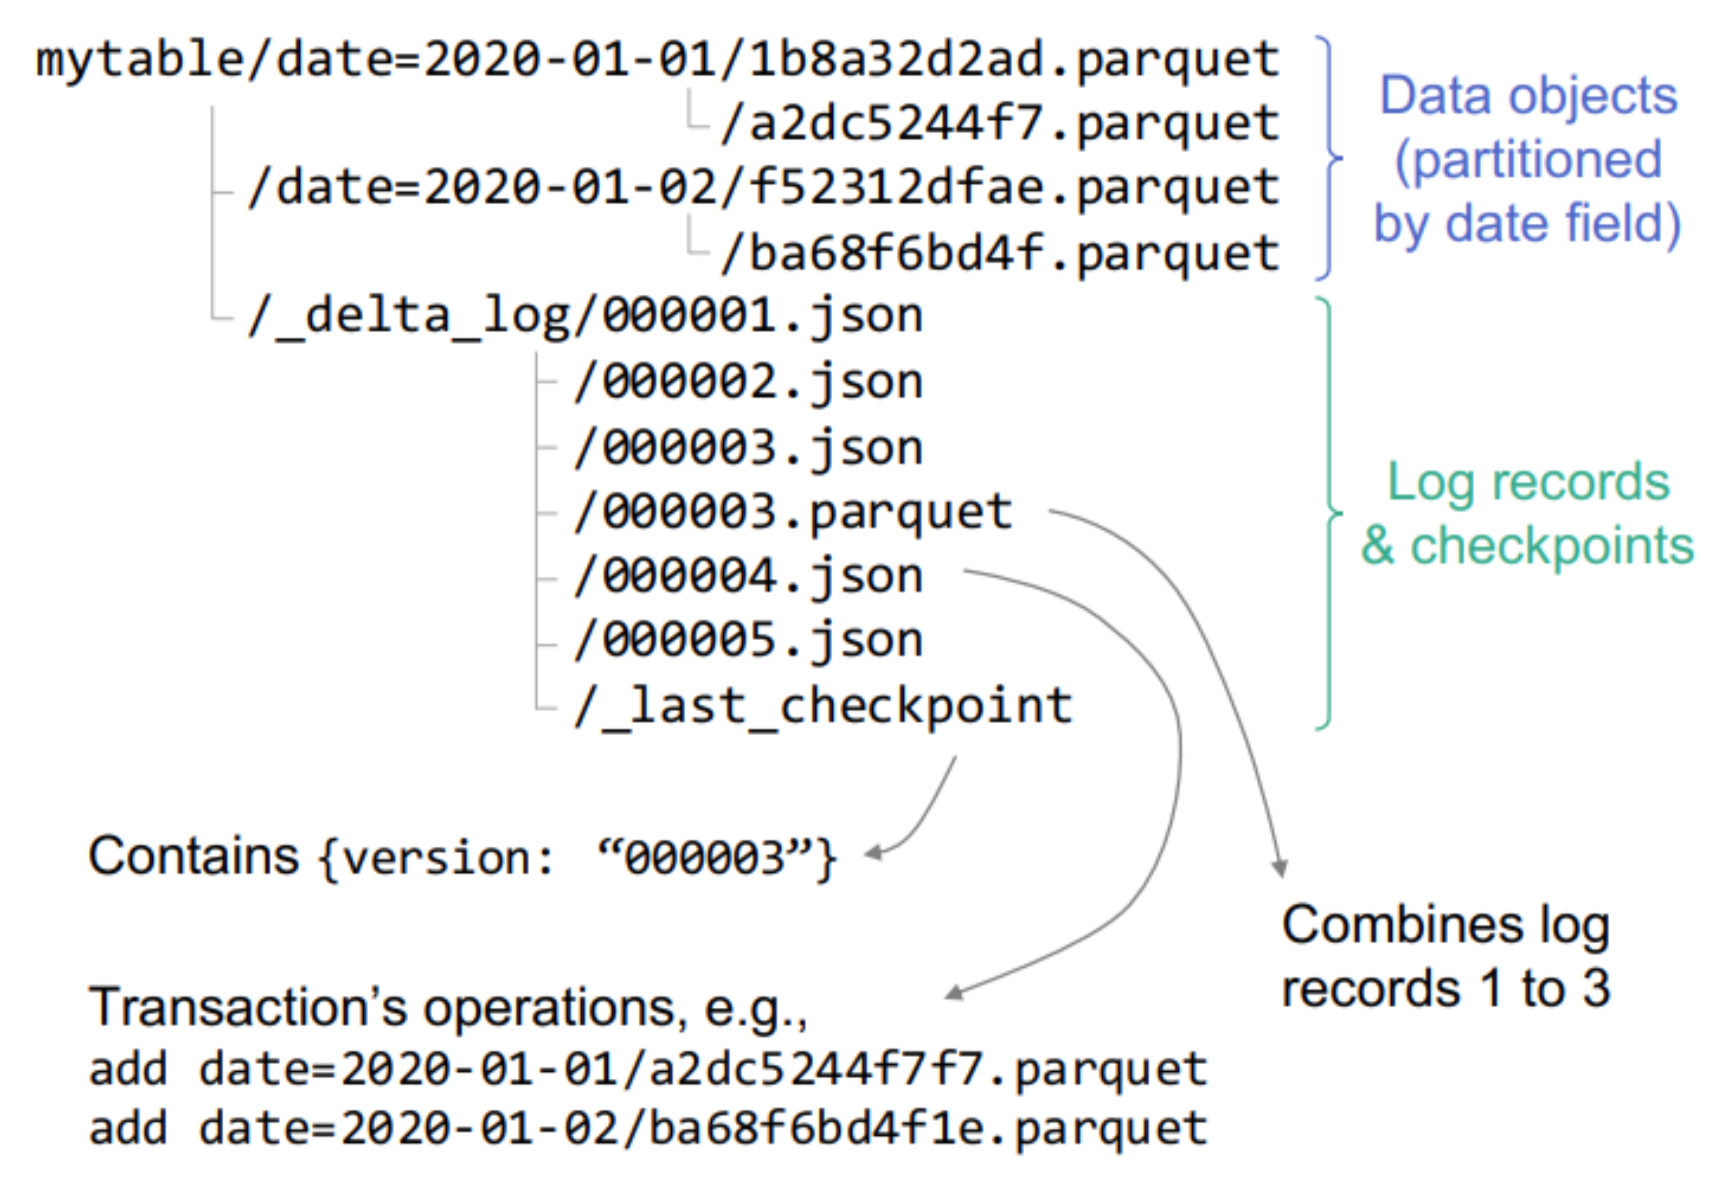
\includegraphics[width=\textwidth]{figures/2-background/delta_lake_table.png}
    \end{center}
    \caption[Delta lake partitioning]{Delta lake table partitioned according to date field. Figure from the slides of the Data-intensive Computing lectures at KTH by Prof. A. H. Payberah. Course website available at \url{https://www.kth.se/student/kurser/kurs/ID2221?l=en}.}
    \label{fig:delta_table}
\end{figure}

\subsection{Accessing Delta Lake}
\label{subsec:delta_lake_access}

The Delta Lake project is strictly related to Apache Spark, as Databricks (the company that developed Delta Lake) was built by the Spark developers \cite{zaharia2010spark} to offer big data management services around Spark. As of version 3.0 of Delta Lake, Delta Kernel was announced \cite{AnnouncingDeltaLake2023}, a Java library providing low-level access to Delta Lake, without needing to write the Delta Lake logic. While this move tried to standardize all accesses to Delta Lake under the Spark/Java environment, new ways to access the library had already been written since Delta Lake is an open-source project.

As early as April 2020, the Rust community started implementing a new interface to access Delta Lake written in Rust without \gls{JVM} dependencies. This library expanded even more the Delta Lake ecosystem, breaking the dependency between Delta Lake and Spark to perform operations on the data lakehouse. This worked particularly well considering that the data science community makes heavy use of Python and typically would avoid having \gls{JVM} dependencies. Being delta-rs written in Rust it makes the library highly compatible with Python since it can be easily wrapped and deployed as a Python library. This is perhaps the reason behind the fact that delta-rs can be simply installed in Python with the name "deltalake".

\section{Query engine}
    \label{sec:query_engine}
    % Introduction
This section described the technologies used to query, cache, and process data in this project. Query engine refers mainly to Apache Spark and DuckDB, but also the other technologies presented in this chapter operate at the same abstraction level while having different functions.

\subsection{Apache Spark}

Apache Spark (from now on simply Spark) is an open-source distributed computing framework designed to handle large-scale data-intensive applications \cite{zahariaApacheSparkUnified2016}. Spark builds from the roots of MapReduce and its variants. MapReduce is a distributed programming model first designed by Google that enables the management of large datasets \cite{dean2004mapreduce}. The paradigm was later implemented as an open-source project by Yahoo! engineers under the name of Hadoop MapReduce \cite{borthakurHadoopDistributedFile2005}. Spark improved this approach by making use of \glspl{RDD} \cite{Zaharia:EECS-2011-82}. \glspl{RDD} are a distributed memory abstraction that enables a lazy in-memory computation that is tracked through the use of lineage graphs, ultimately increasing fault tolerance \cite{Zaharia:EECS-2011-82}. The difference between Hadoop MapReduce and Spark is represented in Figure \ref{fig:MapReducevsSpark}.

\begin{figure}[!ht]
  \begin{center}
    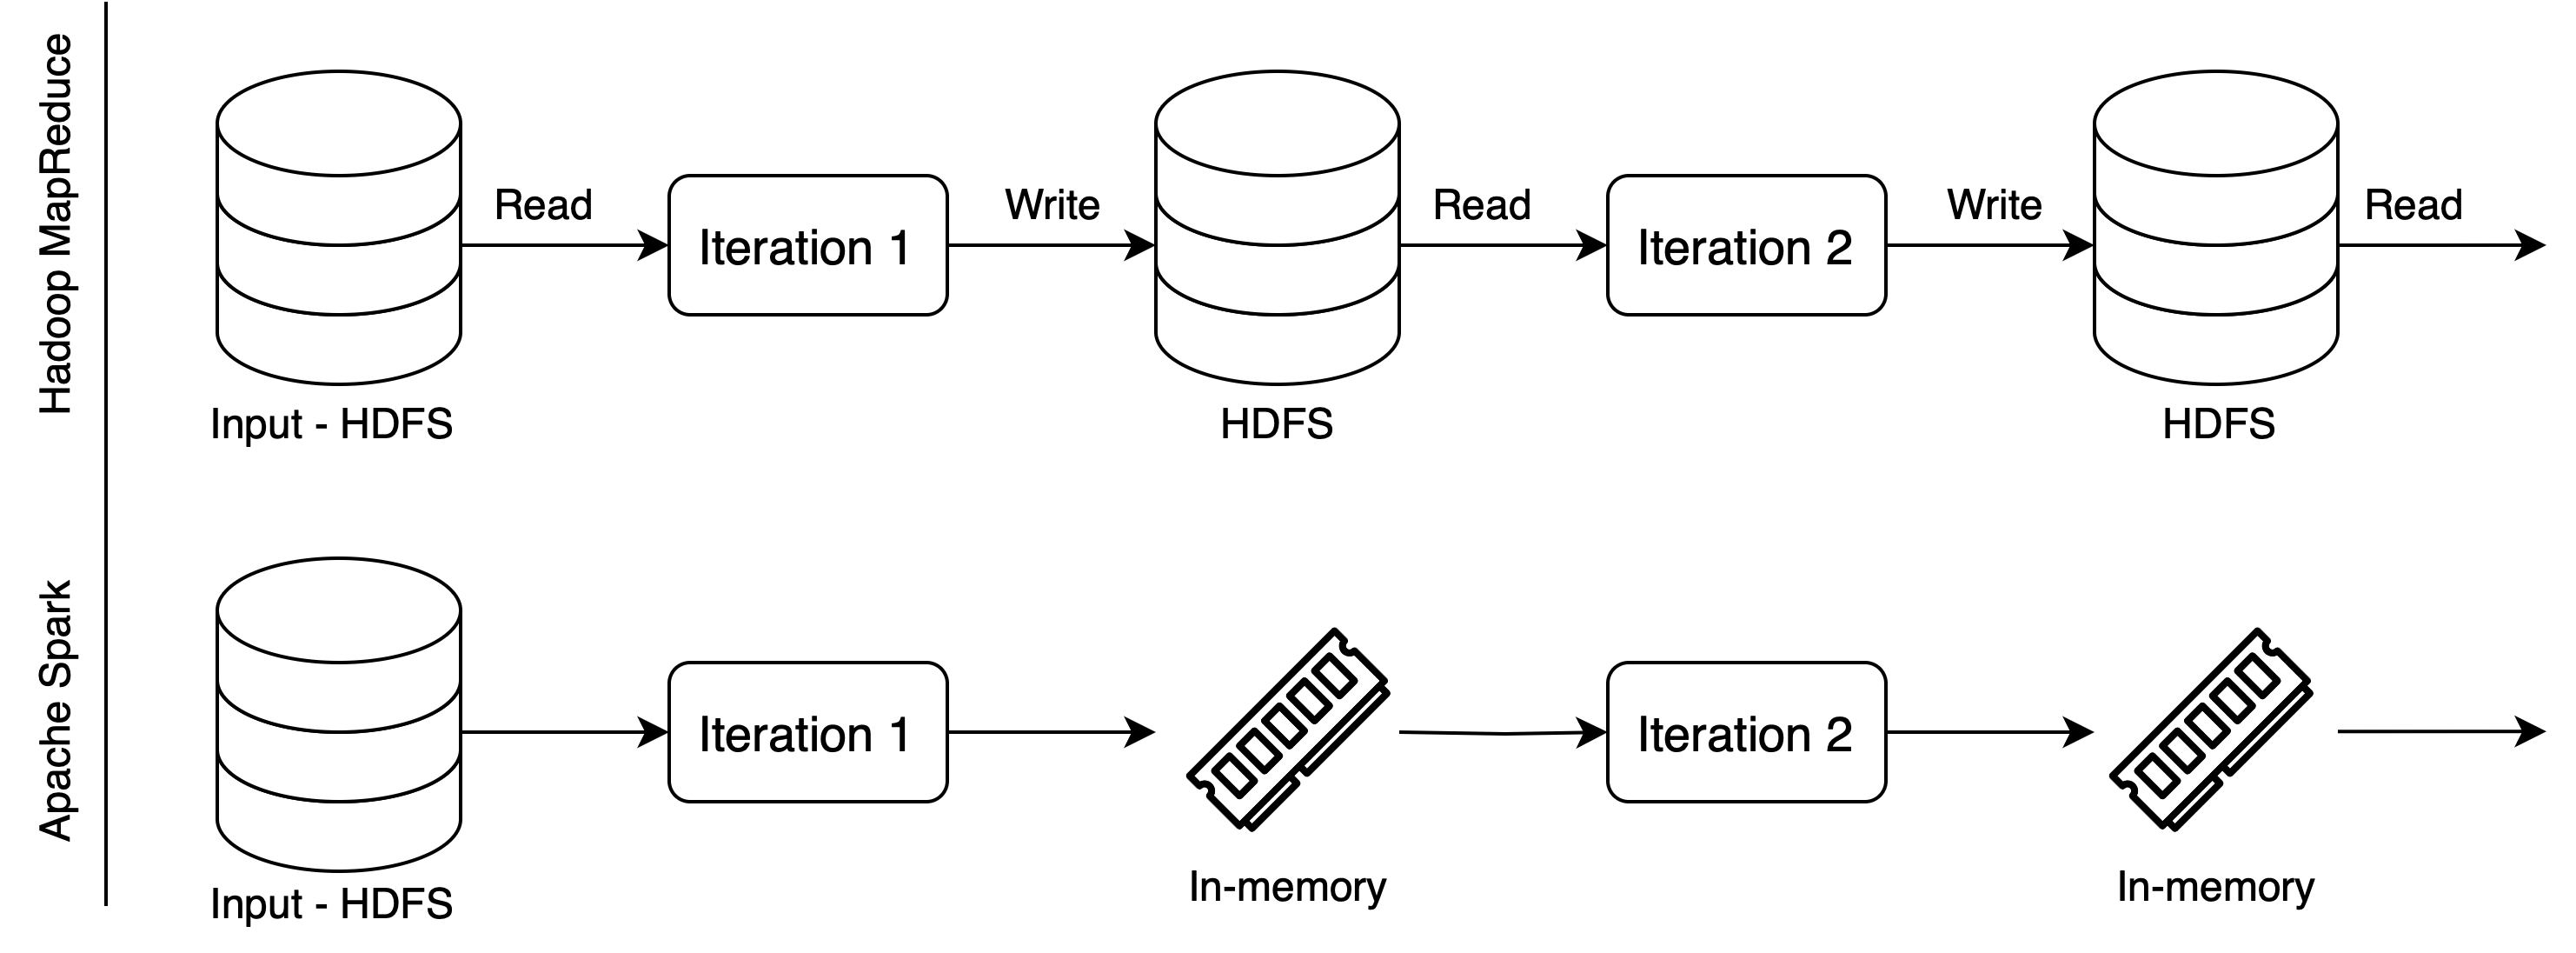
\includegraphics[width=\textwidth]{figures/2-background/Spark_MapReduce.png}
  \end{center}
  \caption{Hadoop MapReduce and Apache Spark execution differences}
  \label{fig:MapReducevsSpark}
\end{figure}

\subsection{Apache Kafka}

Apache Kafka (from now on, Kafka) is an open-source distributed data streaming platform designed for high-throughput, and scalable data processing \cite{krepsKafkaDistributedMessaging2011}. Kafka is most typically used for real-time streaming applications thanks to low latency. 

\begin{figure}[!ht]
    \begin{center}
      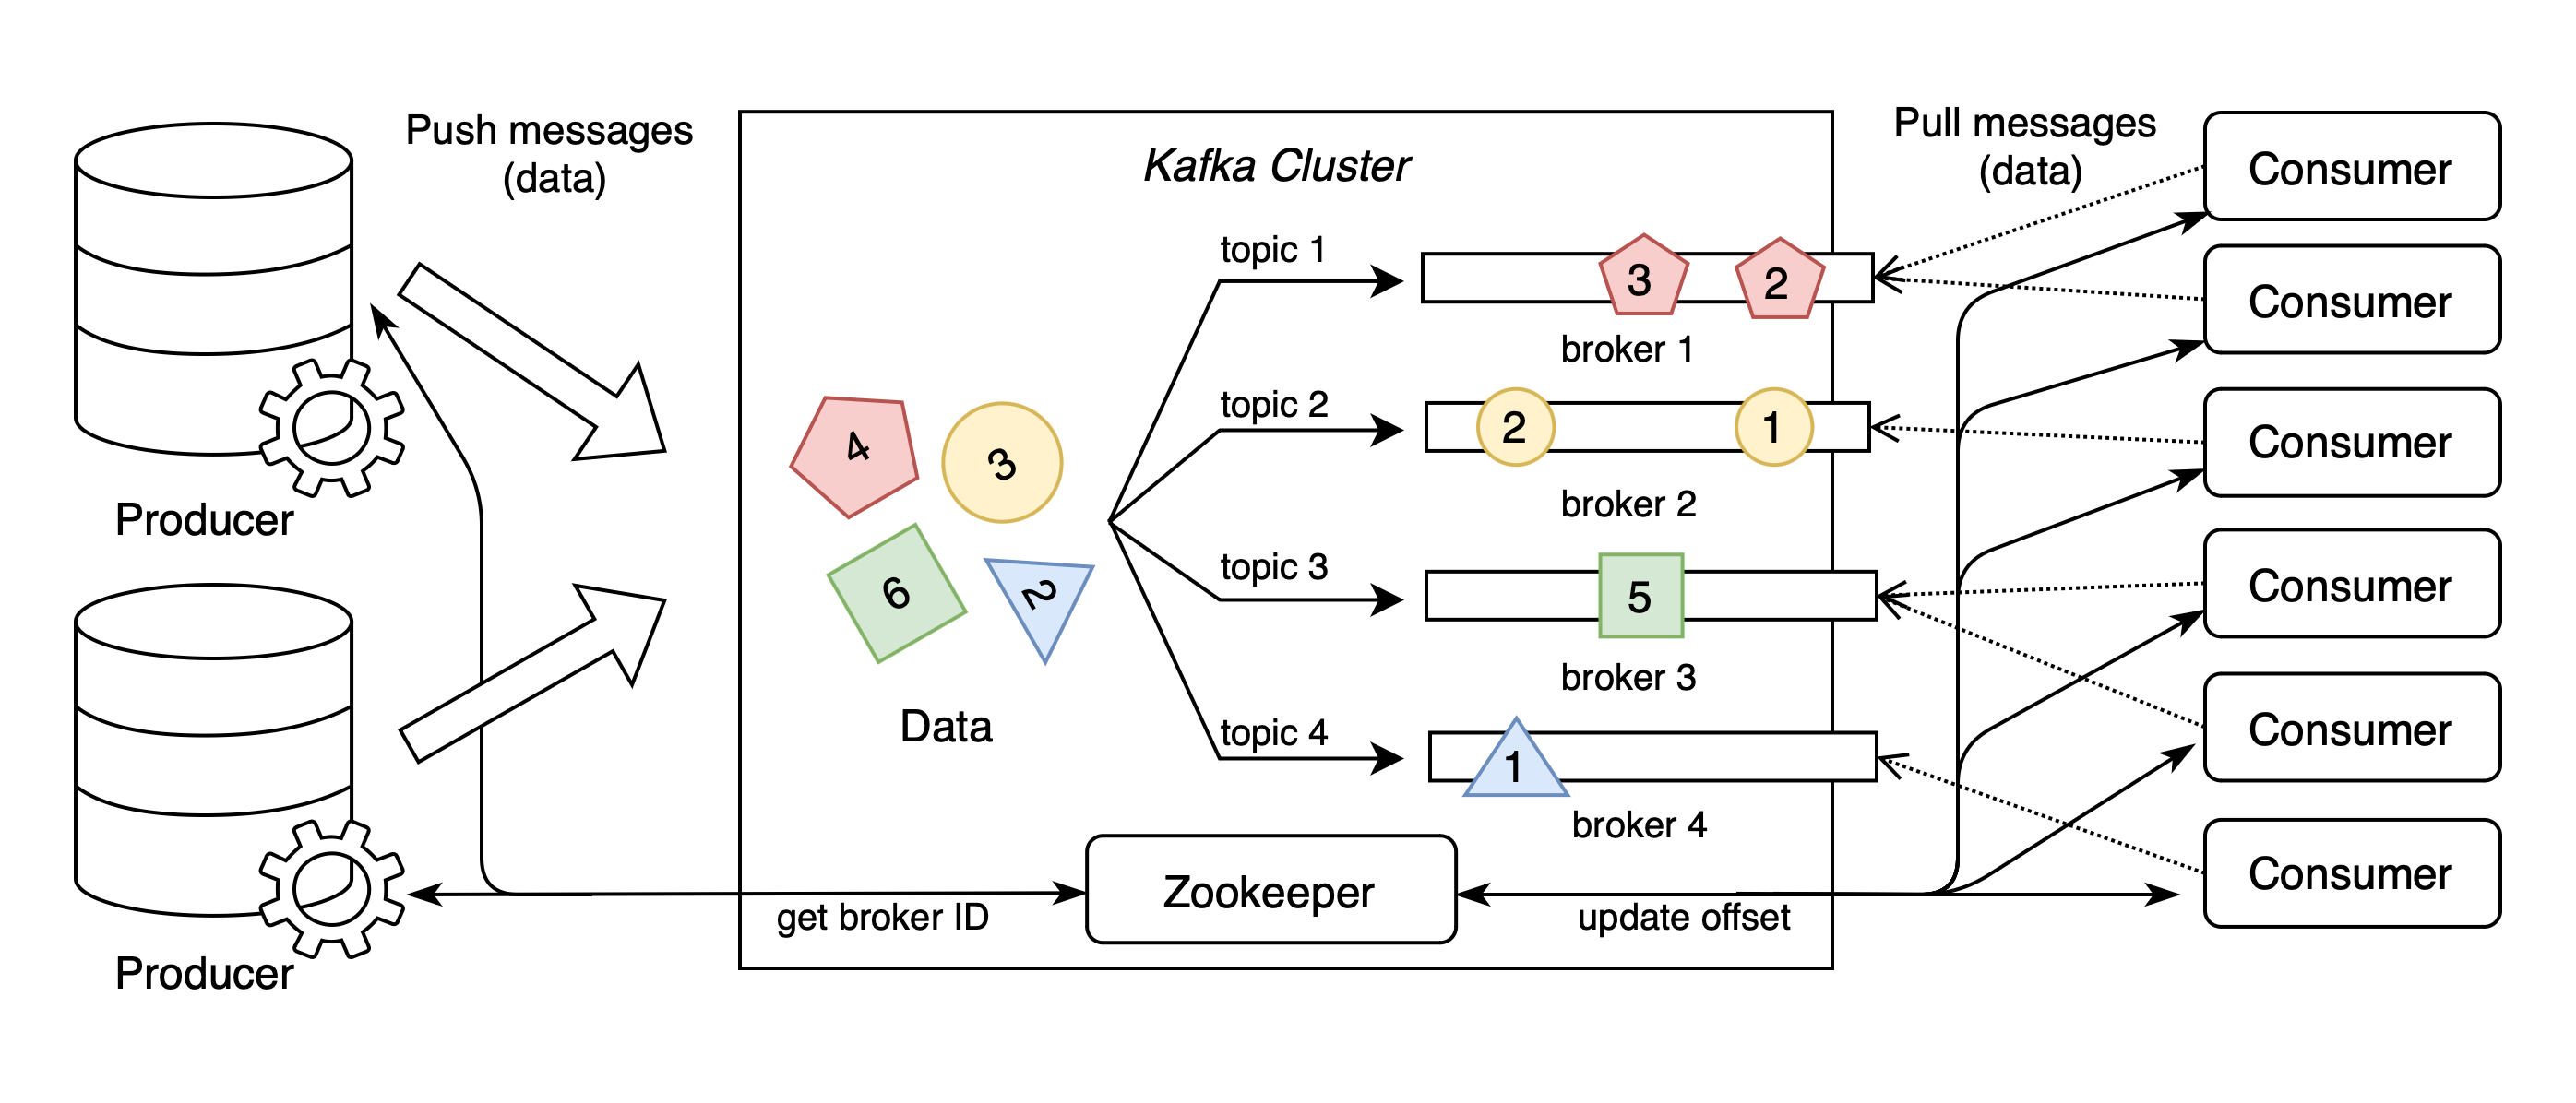
\includegraphics[width=\textwidth]{figures/2-background/kafka.png}
    \end{center}
    \caption{Kafka cluster}
    \label{fig:kafka}
\end{figure}

Figure \ref{fig:kafka} shows the components and messages exchanged in a Kafka cluster. The key components of Kafka are:
\begin{enumerate}
    \item \textbf{Producer}: an application that produces and labels data with specific topics (shapes in the figure).
    \item \textbf{Zookeeper}: responsible for keeping track of brokers and the topic's current offset.
    \item \textbf{Broker}: a computational node (or server) that handles data on a specific topic. It is responsible for receiving messages from producers. Once messages are received the broker forwards them on request by the consumers. This enables the asynchronous protocol.
    \item \textbf{Consumer}: an application that is interested in topic-specific data. To access data it is subscribed to a topic receiving new messages when published. To a topic, more consumers can be subscribed.
\end{enumerate}

The protocol allows applications acting as producers and consumers to avoid having a synchronous protocol. This enables producer's high throughput since they can send messages without waiting for consumers to process them. This also allows consumers to be flexible on workload size.

Given its distributed nature, Kafka allows several producers, consumers, and brokers to exist at the same time. This enables the system to be tuned according to the needs of a specific application. 

\subsection{DuckDB}

DuckDB \cite{raasveldtDuckDBEmbeddableAnalytical2019} is an open-source, embedded, \gls{OLAP} \gls{DBMS}. DuckDB was designed to process small quantities of data (1 - 100 GBs) within the same process or application that runs it, instead of a different process/application. These features create an efficient \gls{OLAP} database that can be used for data analysis, and data processing on a small scale, without the complexity of a more complex \gls{DBMS}, e.g. Teradata \cite{shahImproveYourOLAP}. 

The light structure that characterizes DuckDB is what enables this system to be extremely responsive with low latency. The limitations of the system regard data size, as DuckDB makes use of in-memory processing, it is not able to handle big workloads (1TB or more), which require multiple disk loads.

\subsection{Arrow Flight}

Arrow Flight is a high-performance framework for data transferring over a network, most typically Arrow tables \cite{wesmIntroducingApacheArrow2019}. This protocol enables the transfer of large quantities of data stored in a format, e.g. Arrow tables, without having to serialize or deserialize it for transfer. This speeds up the data transfer by a large margin making Arrow Flight extremely efficient. Arrow Flight is designed to be cross-platform, having support for multiple programming languages (C++, Python, Java). The protocol also supports parallelism, speeding up transfers by using multiple nodes on parallel systems. Arrow Flight protocol is built on top of gRPC \cite{GRPC}, enabling standardization and an easier development of connectors. 

\section{Application - Hopsworks feature store}
    \label{sec:hopswoks_feature_store}
    % Introduction
This section describes the application layer which takes advantage of the data stack described. The software described is the Hopsworks Feature Store, that this project contributes to.

\subsection{MLOps fundamental concepts}

\gls{MLOps} are a set of practices to automate and simplify \gls{ML} workflows from the data collection, to the model deployment. \gls{MLOps} considers the problem of developing and deploying a \gls{ML} system from a code point of view, and data point of view. While for a typical software application, only code needs versioning, for a \gls{ML} application also data needs versioning, as training on different data versions might affect performance. The need for data versioning saw Feature Store emerge as a solution for the problem \cite{MeetMichelangeloUbers2017}. Feature store play a central role in the \gls{MLOps} process, serving as fast-access storage during the process.

Figure \ref{fig:mlops} shows a simple \gls{MLOps} architecture making use of the Hopsworks' AI data platform. After data is gathered from various sources, a feature pipeline process the data performing model-independent transformations and saving the resulting features in the Feature store. The training pipeline then runs model dependent transformation (based on the specific model that is going to be trained), on the same features retrieved from the Feature Store and save the output, i.e. the model in a Model registry. Then a last process is responsible for performing inference, and it is typically embedded in deployed applications. For this process it will be enough to take the new features gathered on the platform and perform and inference on the specific model saved in the Model registry.

This type of architecture allows a asynchronous decoupled pipeline that enables the system to be maintainable, scalable and extremely effective for production scenarios.

\begin{figure}[!ht]
    \begin{center}
      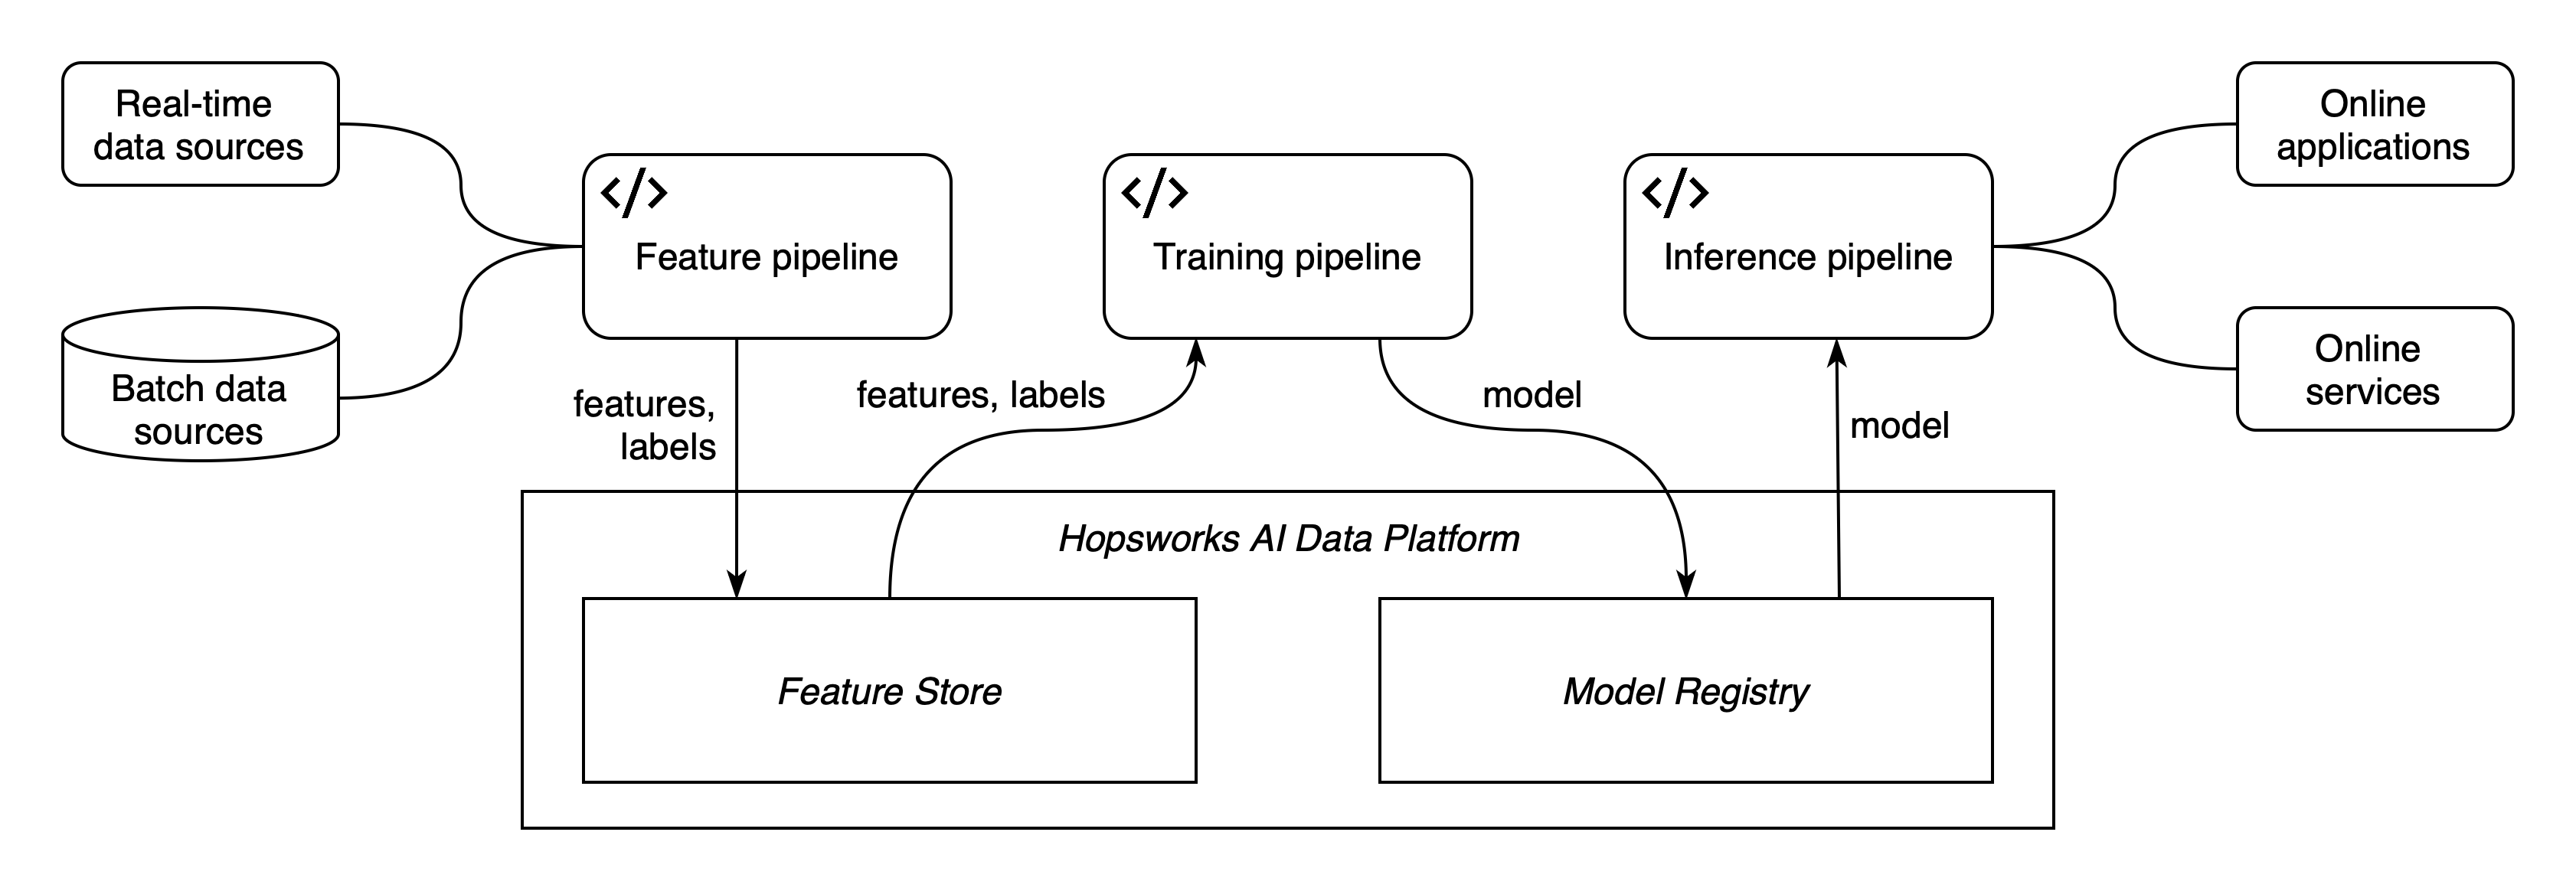
\includegraphics[width=\textwidth]{figures/2-background/MLOps.png}
    \end{center}
    \caption{\glstext{MLOps} pipeline using a Feature Store and a Model Registry}
    \label{fig:mlops}
\end{figure}


\subsection{Hopsworks Feature Store}

As first introduced in the previous section, the Feature Store is a key data layer in an \gls{MLOps} workflow. Feature Store enable features reusability, a centralized and easier collaboration on model training and deployment. The Hopsworks Feature Store organizes features in feature groups, i.e. a mutable collection of features. Feature groups can be queried via the Hopsworks \gls{API} allowing developers to perform \gls{CRUD} operations.

The Hopsworks Feature Store in addition to supporting batch data sources also supports real-time data streaming. To be able to support both systems (or hybrids), the Hopsworks Feature Store saves features in two storages: the Offline Feature Store and the Online Feature Store. The Offline feature store is a column-based storage suited for batch data, that is updated with a low frequency (every few hours at maximum frequency). The Online feature store on the other hand is a row-based, key-value, data storage based on RonDB \cite{LogicalclocksRondb2024}. These characteristics enable low latency and real time (in seconds) data processing. To keep this dual system consistent the Hopsworks Feature Store has a unique point of entry for data which is Kafka, that guarantees at least one message delivery to both storages. This enables the system to support both workflows while keeping a consistent data storage.

\section{System architectures}
    \label{sec:arch_sys}
    % Intro
This section describes the architectures of the legacy and new systems that will be run and measured in the experimental part of this thesis. The section is divided into four sections and each schema presented shows the protocol step by step.

\subsection{Legacy system - Writing}
\label{subsec:legacy_sys_writing}

Figure \ref{fig:featurestore_writing}~\footnote{For enhanced visualization, refer Figure~\ref{fig:appx_featurestore_writing}} shows the legacy Hopsworks Feature Store write process from the client onto the Offline Feature Store. The process is mainly split into two synchronous parts: upload and materialization. In the upload step, the Pandas data frame given as input is converted into rows and sent one row at a time to Kafka. Then, when the upload is finished the client is notified. Asynchronously, a Spark job has been running in the cluster since the Hopsworks cluster was started, which is the Hudi Delta Streamer. This job periodically retrieves messages from Kafka, and then once it retrieves a full table it writes it in a column-oriented format to Apache Hudi, which sits on top of a \gls{HopsFS} system. Once the materialization is completed the Python client is also notified of completion.

As in the pipeline, the upload and the materialization are two different parts of the process that do not act synchronously. During the experimental part of the thesis, to be able to measure the latency of the whole process without having to account for the Hudi Delta Streamer data retrieval period, the materialize function was called, which allows the system to perform the materialization on call instead of waiting for the period. This enabled the experiments to retrieve accurate data on the total latency of the process.

\begin{figure}
    \begin{center}
      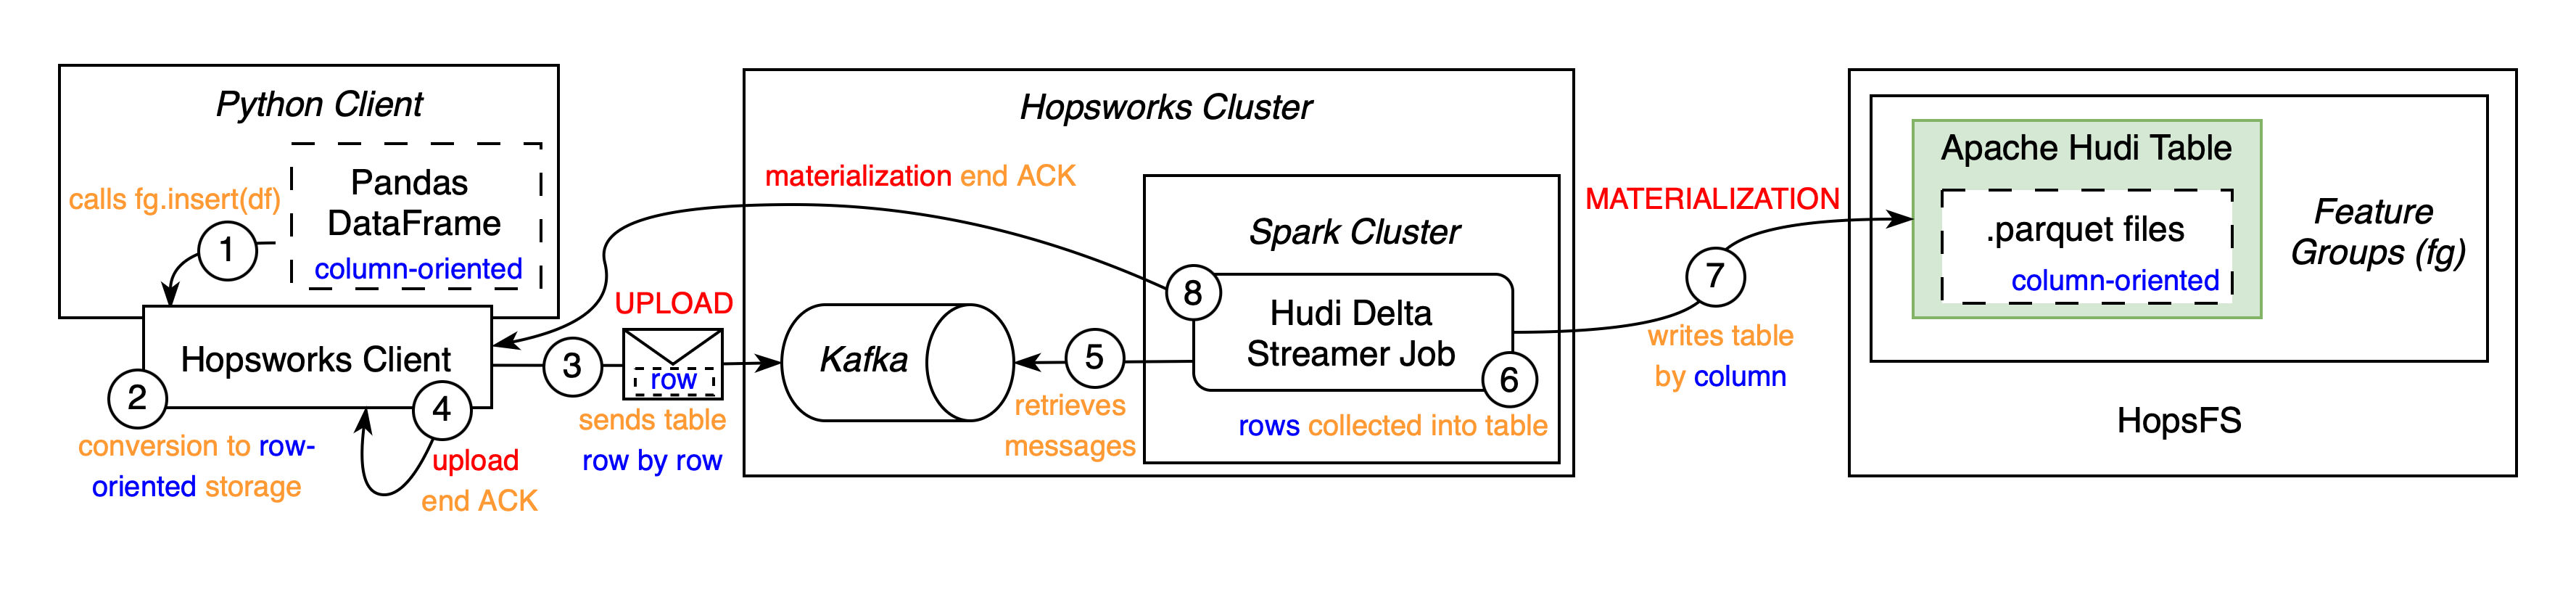
\includegraphics[width=\textwidth]{figures/2-background/FeatureStore-writing.png}
    \end{center}
    \caption[Legacy system - Write process]{Legacy system writing a Pandas data frame from a Python client to the Hopsworks offline Feature Store. Each step is represented with a number. In blue it is outlined the table format conversion, i.e. from columns to rows and then from row to columns. Steps from one to four represent the upload process, while the materialization process in complete at step eight. Diagram realized based on one-to-one interviews with Hopsworks AB employees developing the Hopsworks Feature Store.}
    \label{fig:featurestore_writing}
\end{figure}

\subsection{Legacy system - Reading}
\label{subsec:legacy_sys_reading}

Figure \ref{fig:featurestore_reading}~\footnote{For enhanced visualization, refer Figure~\ref{fig:appx_featurestore_reading}} shows the legacy Hopsworks Feature Store read process from the client onto the Offline Feature Store. The process, differently from the writing process, is not Spark-based and it is using a Spark alternative: a combination of an Arrow Flight server and a DuckDB instance. This avoids the serialization and deserialization into row-based tables for sending the data, keeping the unified standard Arrow Table, which is a column-oriented format.

\begin{figure}
    \begin{center}
      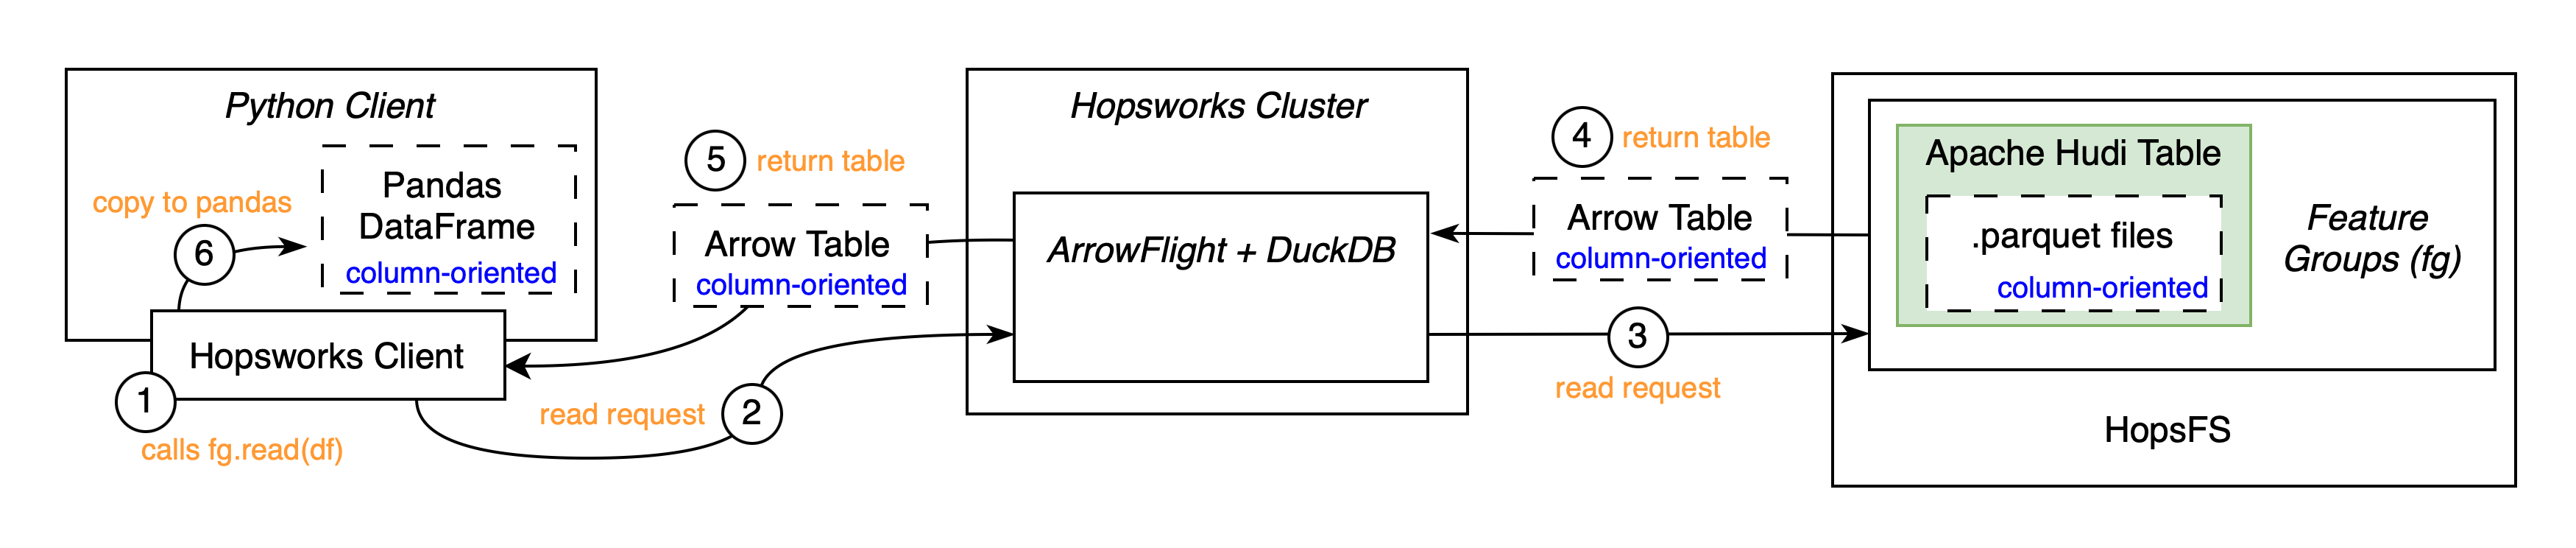
\includegraphics[width=\textwidth]{figures/2-background/FeatureStore-reading.png}
    \end{center}
    \caption[Legacy system - Read process]{Legacy system reading a table from the Hopsworks offline feature store and loading it into the Python client local memory. The process is streamlined using Arrow Tables that avoid table serialization and deserialization. Diagram inspired by the Hopsworks Feature Store paper \cite{10.1145/3626246.3653389}.}
    \label{fig:featurestore_reading}
\end{figure}

\subsection{New system - Writing}

Figure \ref{fig:delta_rs_writing} shows how the delta-rs library writes on a Delta Lake table instanced on top of \gls{HopsFS}. The delta-rs library streamlines the process, without having to pass from a server instance (Spark).

\begin{figure}
    \begin{center}
      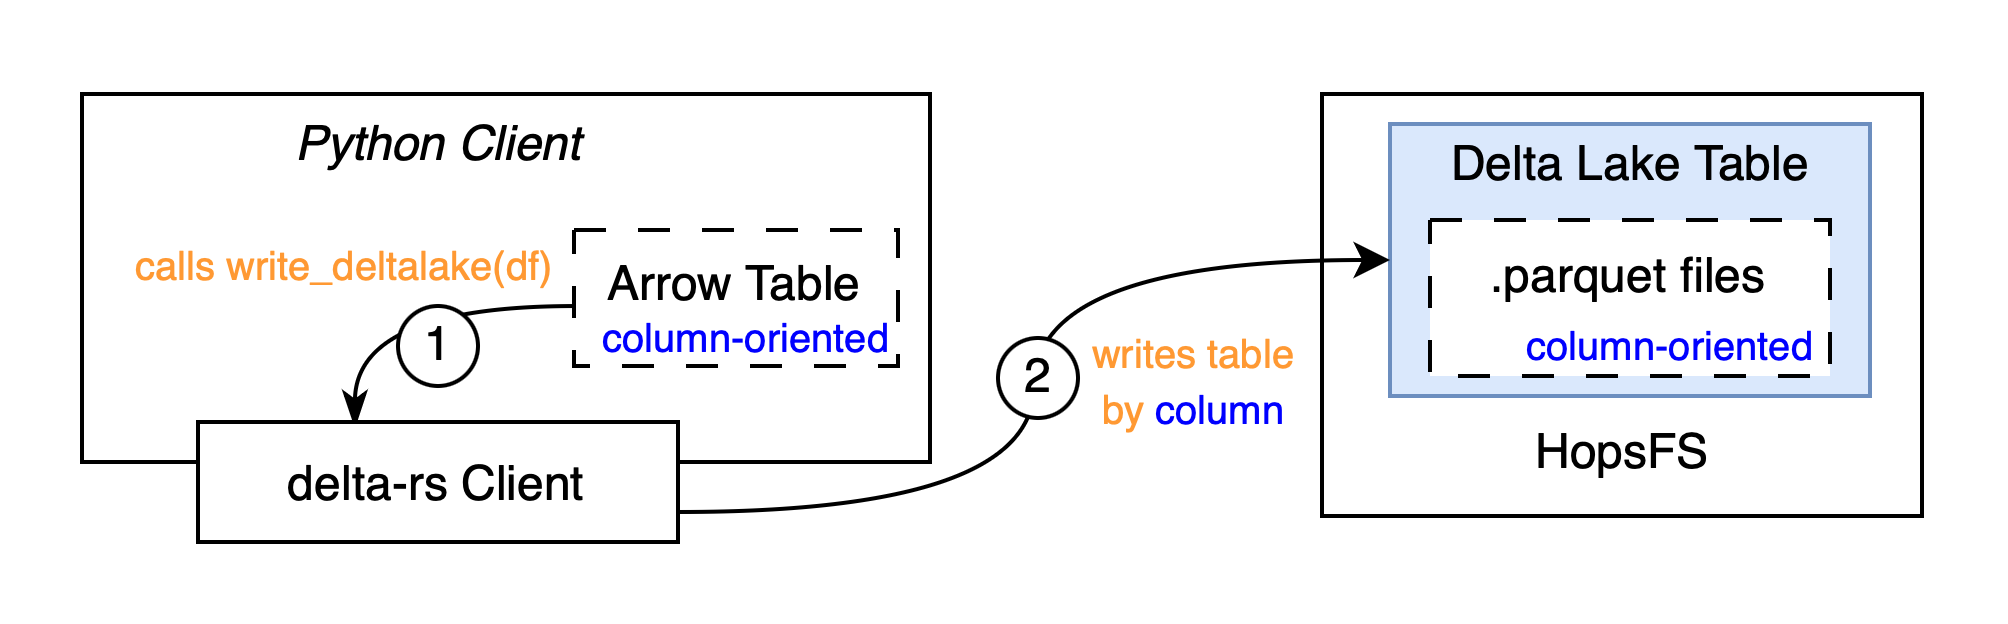
\includegraphics[width=\textwidth]{figures/2-background/delta-rs_writing.png}
    \end{center}
    \caption[Delta-rs library - Write process]{Delta-rs library writing an Arrow Table from a Python client to a Delta Lake table store on \gls{HopsFS}.}
    \label{fig:delta_rs_writing}
\end{figure}

\subsection{New system - Reading}

Figure \ref{fig:delta_rs_reading} shows how the delta-rs library reads on a Delta Lake table instanced on top of \gls{HopsFS}. The delta-rs library streamlines the process, without having to pass from a server instance (Arrow Flight).

\begin{figure}
    \begin{center}
      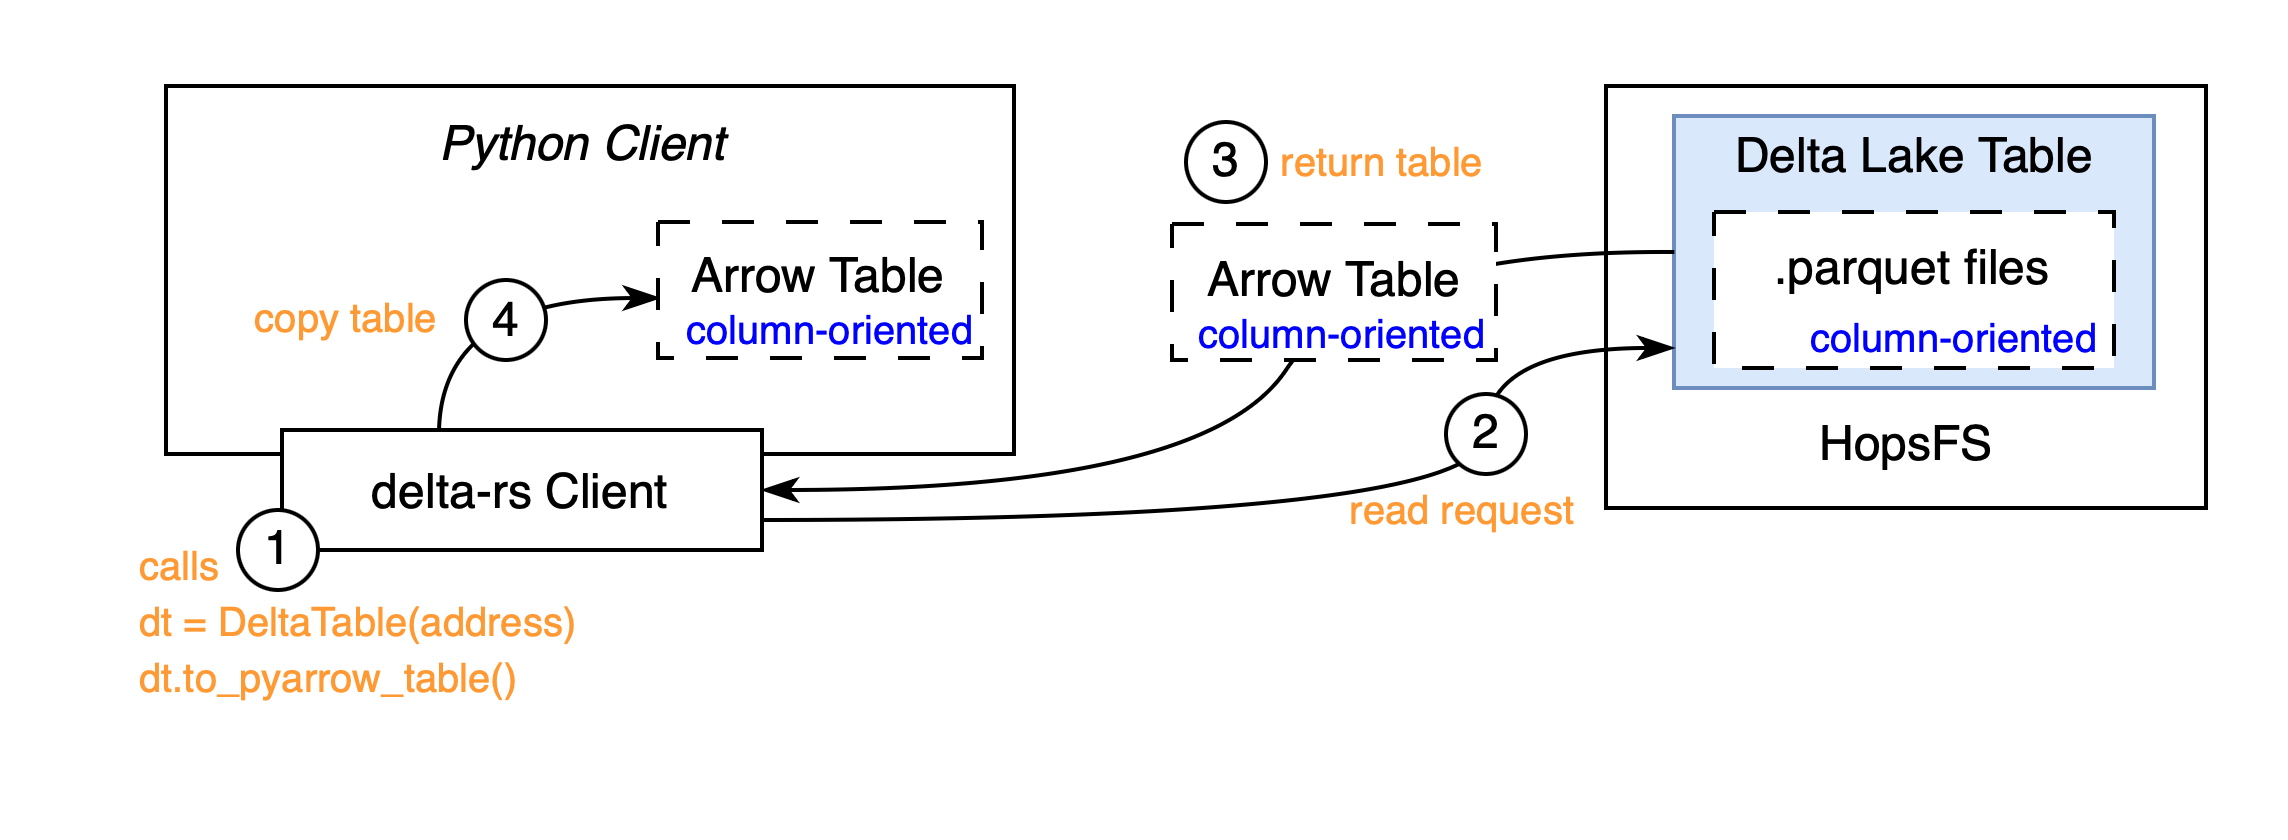
\includegraphics[width=\textwidth]{figures/2-background/delta-rs_reading.png}
    \end{center}
    \caption[Delta-rs library - Read process]{Delta-rs library reading a Delta Table stored in \gls{HopsFS} and loading it into memory.}
    \label{fig:delta_rs_reading}
\end{figure}

%\section{Programming Languages}
%    \label{sec:programming_languages}
%    % Introduction

\subsection{Python}


\subsection{Java}


\subsection{Rust}



\cleardoublepage

\chapter{Method}
    \label{ch:method}
    %Summary of the method section here
This chapter following the two \glspl{RQ} defined in Section \ref{subsec:researchQuestion} defines two methodologies that will be applied sequentially in this project. Section \ref{sec:sys_impl} defines the system implementation process which outputs the D1, i.e. the code implementation, that will enable the system evaluation defined in Section \ref{sec:sys_eval} which will output D2, i.e. the results of the experiment which analysis will be delivered in D3.

\section{System implementation -- RQ1}
  \label{sec:sys_impl}
  % Summary sys_impl here
The core of this system research thesis resides in the system implementation section, which answers RQ1.

This section explains the method and the principles used to carry out the software development process of adding support for \gls{HDFS} and \gls{HopsFS} to the delta-rs library. This section is divided into four sub-sections: Research paradigm, explaining the research framework that will be used to implement the system; Development process, describing the activities that will be carried out to implement the system; Requirements, defining the functional and non-functional requirements of the system and Development environment, detailing the tools and resources that will be used during the development process.

\subsection{Research Paradigm}
The research paradigm of the system implementation section of this thesis is positivist, believing that reality is certain and can be measured and understood. 
In the context of the development process, this research paradigm means that the new system requirements can be defined, and implementation errors can be outlined, understood, and, if possible, fixed. This approach leads to a strict definition of the development process, which depends on functional requirements that must be fulfilled.

\subsection{Development process}
\label{subsec:dev_process}
The development process will follow an iterative and incremental approach described in Figure \ref{fig:DevProcessRQ1}. This methodology will be applied as it allows flexibility while creating incrementally a working system \cite{despa2014comparative}. This project will require numerous interactions with \gls{HopsFS} maintainers (i.e., the industrial supervisor) due to the need for the delta-rs library to interact with \gls{HopsFS}. This review process creates the need for a feedback loop, allowing the system to fit all the requirements according to all stakeholder's expectations.

As it can be noted from Figure \ref{fig:DevProcessRQ1}, each step of this process is related to one of the goals (G1--G4) associated with RQ1 in Section \ref{sec:goals}.
The activities and the relationship between each activity and the associated goal(s) are explained here below:
\begin{enumerate}
    \item \textbf{Identify problems collaboratively}: this activity partially solves G1--G2, as it is an initial system analysis, performed together with the industrial supervisor, who is knowledgeable on Hopsworks' infrastructure (in particular \gls{HopsFS}). This task fixes the project's initial requirements and investigates what needs to be implemented at a high-level abstraction.
    \item \textbf{Analyse system}: this activity partially solves G1--G2 each time it is re-iterated, as it performs low-level code-based analysis of how the system works and what needs to be implemented to support \gls{HDFS} in delta-rs. This activity also starts an iterative loop that will end once the system fulfills the requirements described in Section \ref{subsec:requirements}.
    \item \textbf{Design software}: this activity solves partially G3, as the first part of the software development. In this activity, a solution is designed from the information gathered in the system analysis.
    \item \textbf{Code software}: this activity solves partially G3, as the second part of the software development. In this activity, the solution designed is coded.
    \item \textbf{Test system}: this activity partially solves G4, as the first part of the tests performed to verify the solution validity via unit tests. Failed unit tests will trigger a new development loop iteration, where this failure will be considered as the first starting point in the system analysis.
    \item \textbf{Verify system integration}: this activity partially solves G4, as the second part of the tests performed to verify the solution validity via integration tests. Failed integration tests will trigger a new development loop iteration, where this failure will be considered as the first starting point in the system analysis. On the other hand, if the integration test succeeds, the loop will be restarted if the system does not yet fit a requirement. Otherwise, the development process finishes if the system fulfills all the functional requirements described in Section \ref{subsec:requirements}.
\end{enumerate}

This process will produce a final deliverable (D1), which is a Python wheel of the delta-rs library containing the support for \gls{HDFS} and \gls{HopsFS}.

\begin{figure}[!ht]
    \begin{center}
      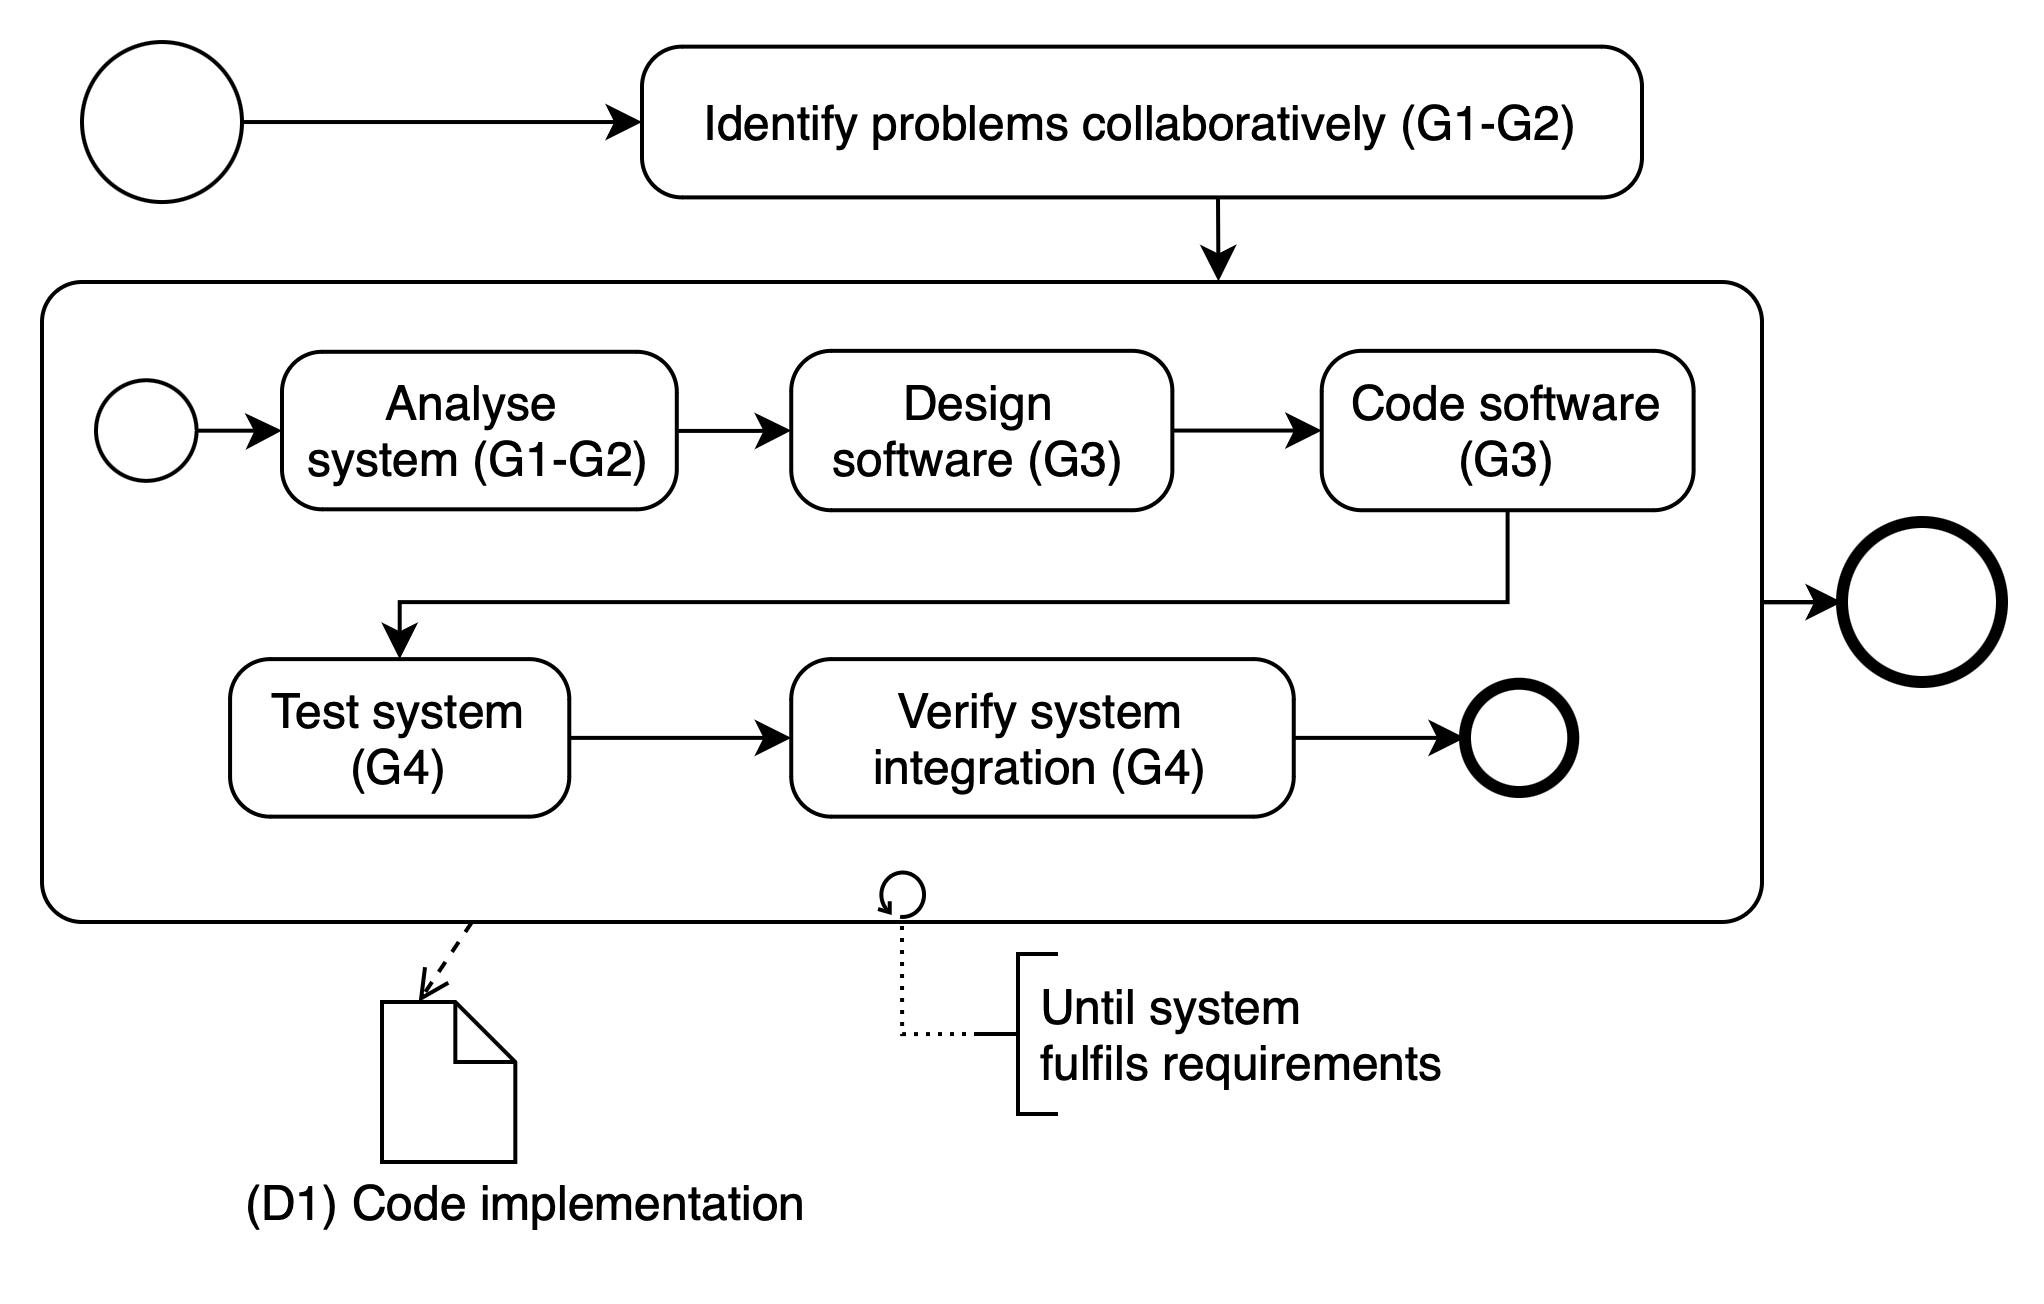
\includegraphics[width=\textwidth]{figures/3-method/research_process_rq1.png}
    \caption[System implementation process]{\gls{BPMN} diagram of the System implementation process answering to RQ1. Each activity is associated with a specific Goal (\gls{G}). The process produces a deliverable (\gls{D}), in this case, a code implementation. The development loop iterates until the functional requirements (defined in Section \ref{subsec:requirements}) are fulfilled.}
    \label{fig:DevProcessRQ1}
    \end{center}
\end{figure}

\subsection{Requirements}
\label{subsec:requirements}
In the first steps of the system analysis, a series of requirements are defined in agreement with the industrial partner Hopsworks \gls{AB} to favor the creation of a solution that could be later used within the company in a production environment. These are divided into two categories: functional and non-functional requirements. \\ The \textbf{functional requirements} are:
\begin{enumerate}
    \item \textbf{Write Delta Tables}: the solution should allow to write Delta Lake tables on \gls{HopsFS} via the delta-rs library.
    \item \textbf{Read Delta Tables}: the solution should allow to read Delta Lake tables on \gls{HopsFS} via the delta-rs library.
    \item \textbf{Communicate via TLS}: the solution should interact with \gls{HopsFS} via \gls{TLS} protocol version 1.2.
\end{enumerate}
The \textbf{non-functional requirements} are:
\begin{enumerate}
    \item \textbf{Consistent}: the solution should be consistent with the current open-source codebase used when appropriate.
    \item \textbf{Maintainable}: the solution should minimize the need for maintenance and support of the codebase in the future, minimizing changes to open-source code. When appropriate, the solution's changes should be compatible with a future upstream merge to the modified open-source project.
    \item \textbf{Scalable}: the solution should be able to handle larger quantities of data (up to 100 GB) read or written on Delta Tables.
\end{enumerate}

\subsection{Development environment}
The system implementation will be developed by making use of several technologies, here categorized:
\begin{itemize}
    \item \textbf{Computing resources}: the system implementation will be developed in a remote environment accessed via \gls{SSH} from a computer terminal. This remote \gls{VM} is selected as mounting \gls{HopsFS} on a local machine is non-trivial, and developing locally could result in inconsistencies when the solution is reproduced in a virtual environment.
    \item \textbf{Writing code}: the Vim text editor is development tool of choice in combination with \gls{CoC}~\footnote{Project's repository available at \url{https://github.com/neoclide/coc.nvim}} providing language-aware autocompletion and rust-analyzer~\footnote{Project's repository available at \url{https://github.com/fannheyward/coc-rust-analyzer}} access for on-code compiler errors. 
    \item \textbf{Libraries and dependencies}: the environment will be set in a Docker container for more straightforward development and test reproducibility.
    \item \textbf{Code versioning and shared development}: GitHub will be used for versioning, collaborating with open-source projects (e.g., delta-rs), and sharing the developed solution.
\end{itemize}

 

\section{System evaluation -- RQ2}
  \label{sec:sys_eval}
  %Summary here
The system evaluation complements the system implementation by measuring the performance of the developed solution, answering RQ2. This evaluation process will be carried out following a sequential approach.

This section details the method and the principles that will be used to carry out the system evaluation process, measuring the performance (throughput, measured in rows/second) of reading and writing on Delta Lake or Apache Hudi while on \gls{HopsFS} of Spark-based and Rust-based pipelines. 

\subsection{Evaluation Process and Research Paradigm}
\label{subsec:eval_process_and_research_paradigm}

The research process will follow a sequential approach described in Figure \ref{fig:DevProcessRQ2}. Each step of this process is related to one of the goals (G5-G8) associated with the RQ2 in Section \ref{sec:goals}.
The relationship between each activity and the associated goal(s) is here explained:
\begin{enumerate}
    \item \textbf{Design experiments}: this activity maps perfectly to G5, designing the experiments that will be conducted to evaluate the performance difference in performance between Spark-based access to Apache Hudi compared a the delta-rs \cite{DeltaioDeltars2024} library-based access to Delta Lake, in \gls{HopsFS}. 
    \item \textbf{Perform experiments}: this activity maps perfectly to G6, using the code implementation (D1) to conduct the designed experiments on the analyzed systems.
    \item \textbf{Transform data according to metrics}: this activity is necessary to fulfill G7, as data visualization requires data to be properly formatted. In this activity data is modified, performing a division between the size of the table inputted and the read or write time. This allows data to be in the wanted metric i.e. rows/second.
    \item \textbf{Visualise results}: this activity maps perfectly to G7, visualizing the experiments' result according to the selected metric, i.e. throughput measured in rows/second. This activity also generates a deliverable (D2) composed of the experiments results complete with tables and histograms, i.e. Section \ref{}.
    \item \textbf{Analyse results}: this activity maps perfectly to G8, analysing and interpreting the results delivered in D2. This contributes to D3, generating the analysis of results, i.e. Section \ref{}.
\end{enumerate}
\begin{figure}[!ht]
    \begin{center}
      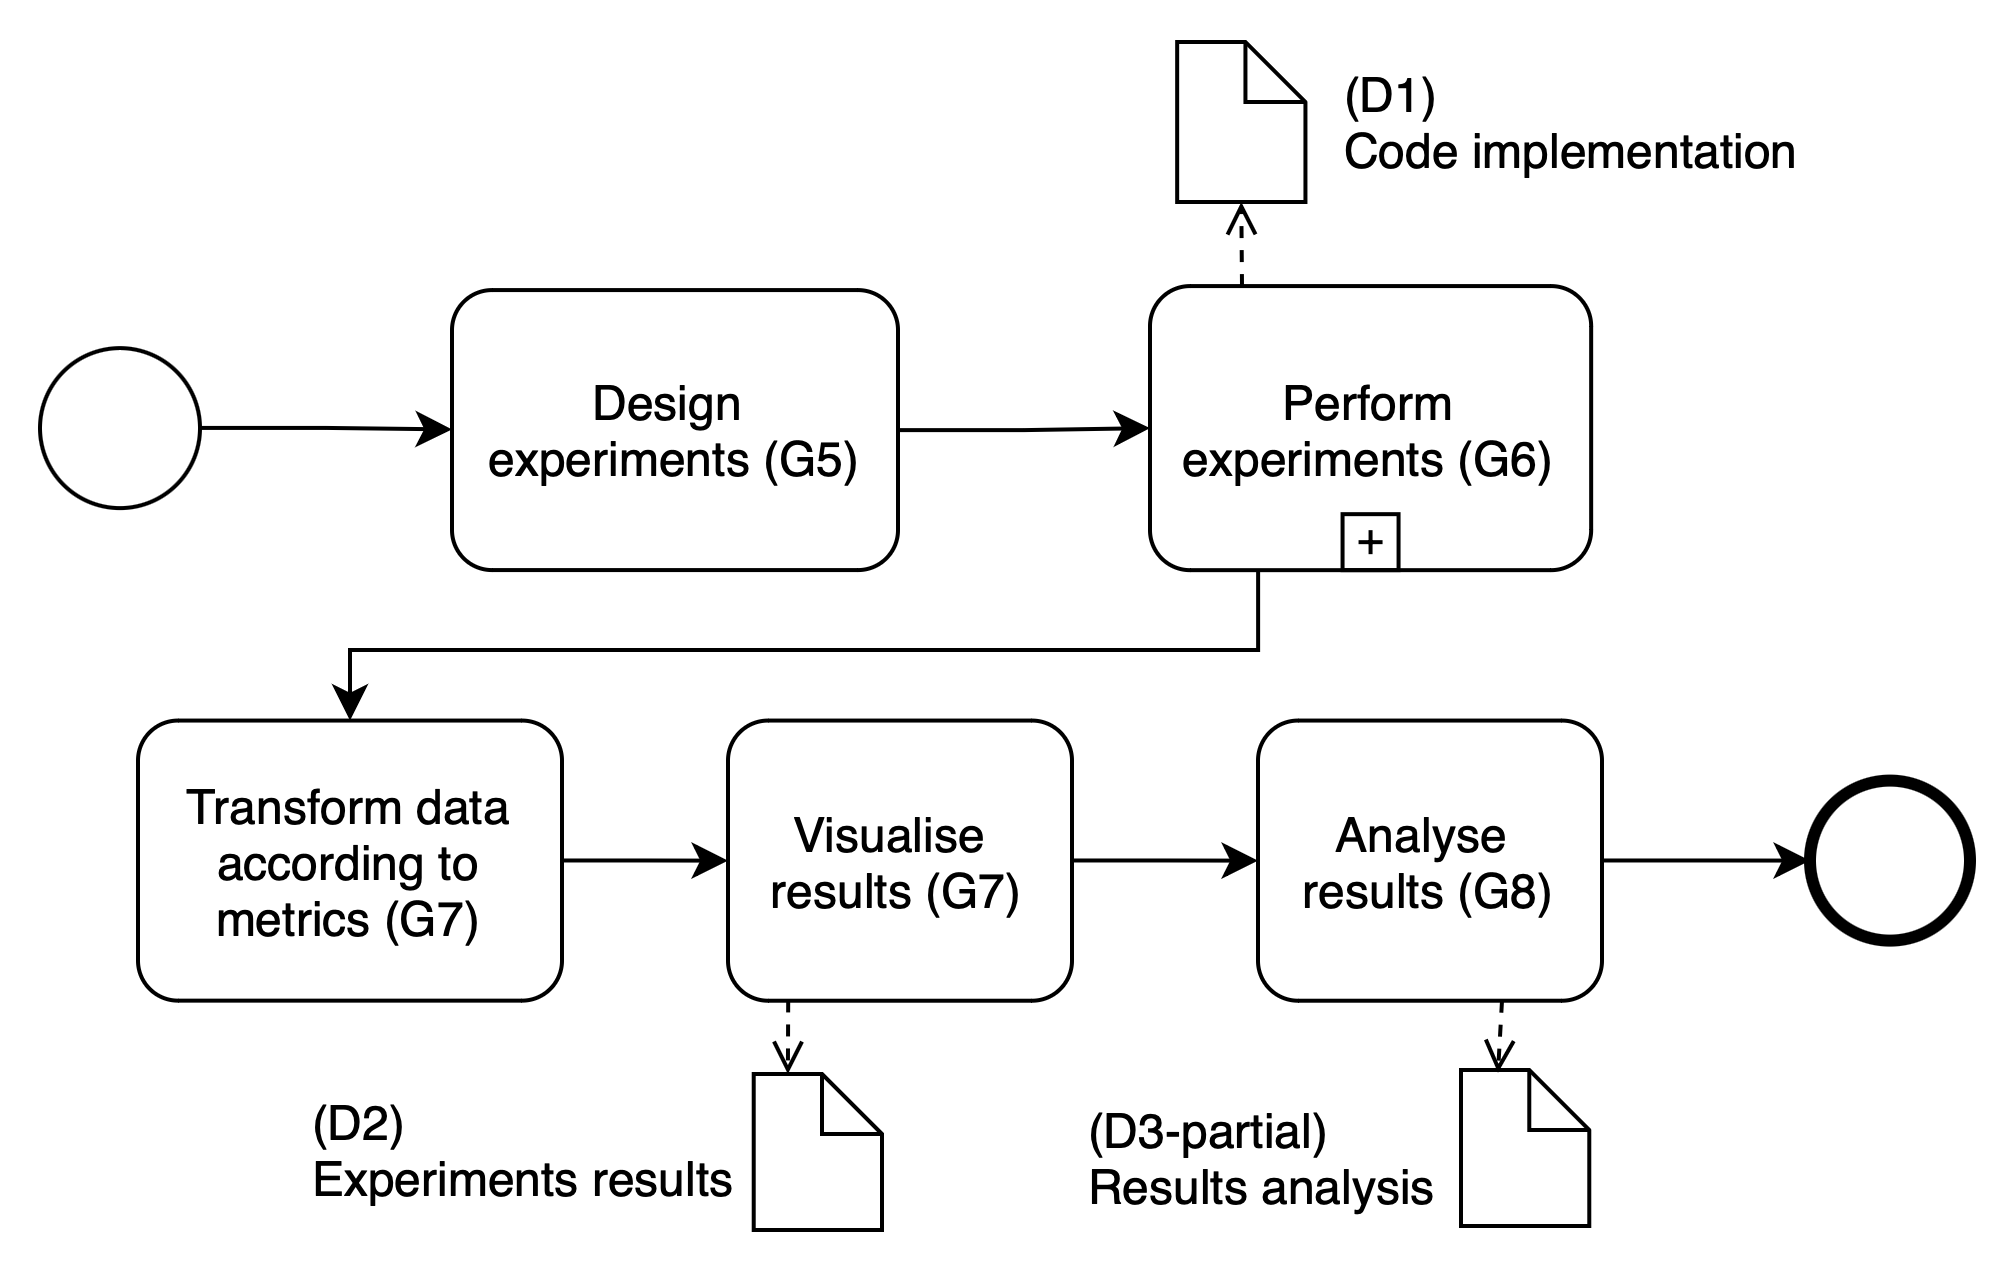
\includegraphics[width=\textwidth]{figures/3-method/research_process_rq2.png}
    \caption{\gls{BPMN} diagram of the System evaluation process answering to RQ2. Each activity is associated with a specific Goal (\gls{G}). The process produces two deliverables (\gls{D}), the experiments results (D2) and a results analysis (D3-partial).}
    \label{fig:DevProcessRQ2}
    \end{center}
\end{figure}

The research paradigm consists of a quantitative analysis based on repeated runs on the implemented system. The results of the benchmarks are then analyzed performing a visual comparative approach.

\subsection{Dataset}
\label{subsec:dataset}

The data that will be used to perform the read and write operations comes from \glsentryshort{TPC}-H benchmark suite\cite{TPCHHomepage}. \glsentryshort{TPC}-H is a decision support benchmark by \gls{TPC}. It consists of a series of business-oriented ad-hoc queries designed to be industry-relevant \cite{transactionprocessingperformancecounciltpcTPCH_v301pdf1993}. The data coming from this benchmark suite was used as
it provides a recognized standard for data storage systems \cite{TPC_benchmarks_2000}, and it has already been used in similar related work \cite{raasveldtDuckDBEmbeddableAnalytical2019, behmPhotonFastQuery2022}. Any part of the data can be generated using the TPC-H data generation tool \cite{TPCCurrentSpecs}.

The \glsentryshort{TPC}-H benchmark contains eight tables, of these two, SUPPLIER and LINEITEM, were selected for the following reasons. The two tables are respectively the smallest (10000 rows) and largest (6000000 rows) tables whose size (number of rows) depends on the \gls{SF}. The \gls{SF} can be varied to obtain tables of different sizes (number of rows), allowing a progressive change in the table size (number of rows). 

The SUPPLIER table has seven columns, while the LINEITEM table has sixteen. This influences the average size of memory each row occupies. This means the metric selected (throughput, measured in rows/second) cannot be used to compare results across different tables. This is the reason why the comparative evaluation only considers different configurations on the same table. 

For this project, five table variations were used to benchmark the code solution as D1. \gls{SF} was varied to obtain a table at each significant figure, from 10000 rows to 60000000 rows. These are the tables:
\begin{enumerate}
    \item \textit{supplier\_sf1}: size = 10000 rows
    \item \textit{supplier\_sf10}: size = 100000 rows
    \item \textit{supplier\_sf100}: size = 1000000 rows
    \item \textit{lineitem\_sf1}: size = 60000000 rows
    \item \textit{lineitem\_sf10}: size = 60000000 rows
\end{enumerate}

\subsection{Experimental Design}
\labe{subsec:experimental_design}
% Description of which benchmarks will be performed and how. Here it needs to be explained the environment where the benchmarks will be run (Snurran), which tests are run and why in this particular way.
%
% Talk about the selection of the questions: How do the performances vary if: (1) the new implemented pipeline is used vs. the old pipeline. (2) a simple localFilesystem implementation is used vs. writing on \gls{HopsFS} (3) varying the CPU configuration (4) we have different table sizes. 

The experiments aim to highlight the differences between the newly implemented system based on the delta-rs library, and the legacy Spark-based system. To isolate the benefit of using delta-rs over Spark and provide a baseline, three different testing pipelines were designed:
\begin{enumerate}
    \item \textbf{delta-rs - \glsentryshort{HopsFS}}: the system implemented in Chapter \ref{ch:implementation}. It comprises a Rust pipeline with Python bindings, enabling performing operations (i.e., reading, writing) on Delta Lake tables. This pipeline writes on \gls{HopsFS}.
    \item \textbf{delta-rs - \glsentryshort{LocalFS}}: this pipeline uses the same library as the system implemented, but saves data on the \gls{LocalFS}. This provides a comparison within the delta-rs library, isolating the impact on performance caused by writing on \gls{HopsFS}, a distributed file system.
    \item \textbf{Legacy Spark pipeline}: this pipeline uses the Hopsworks Feature Store to write data on Hudi tables. This system makes use of a pipeline based on Kafka, and Spark to write data on the Hudi tables, saved on \gls{HopsFS}. 
\end{enumerate}

Furthermore, the experiments will verify how the performances of the three systems will change based on the \gls{CPU} resources provided (namely 1 core, 2 cores, 4 cores, 8 cores). Each time the testing environment will be modified accordingly, creating a new \gls{VM} where the experiments will run with increasingly more resources. These \gls{CPU} configurations were chosen together with the industrial supervisor, according to the typical Hopsworks use case.

The data used for experiments, as described in Section \ref{subsec:dataset}, will come from two different tables. These are modified according to a \gls{SF}, for a total of five times.

In conclusion, the experiments conducted will be a total of 3 (pipelines) times 4 (\gls{CPU} configurations) times 5 (tables) times 2 (read and write operations), i.e. 120 experiments, performed 50 times each to create statistically significant results.

\subsection{Experimental environment}
% Describe Snurran

The experimental environment consists of a physical machine in Hopsworks' offices, virtualized enabling remote shared development. The \gls{CPU} details of the machine are present in Listing \ref{lst:cpu_snurran}, noting that only eight cores at maximum were accessed during the experiments.

The machine mounts about 5.4 TBs of \gls{SSD} memory. This allows the machine to have fast read and write speed, 2.7 GB/s, and 1.9 GB/s respectively (measured with a simple \textit{dd} bash command). 

The experimental environment will be set up with a Jupyter Server of different CPU cores, depending on the experiment (1 core, 2 cores, 4 cores or 8 cores). The Jupyter server is allocated by default with 2048 MB of \gls{RAM}, out of the .. available on the experimental machine. This amount will be adjusted during the experiments according to the needs of the experiments, 

\begin{lstlisting}[language=bash, caption={Output of a \textit{lscpu} bash command on the test environment.}, label={lst:cpu_snurran}, frame=tb]
Architecture:            x86_64
  CPU op-mode(s):        32-bit, 64-bit
  Address sizes:         48 bits physical, 
                         48 bits virtual
  Byte Order:            Little Endian
CPU(s):                  32
  On-line CPU(s) list:   0-31
Vendor ID:               AuthenticAMD
  Model name:            AMD Ryzen Threadripper 
                         PRO 5955WX 16-Cores
    CPU family:          25
    Model:               8
    Thread(s) per core:  2
    Core(s) per socket:  16
    Socket(s):           1
    Stepping:            2
    Frequency boost:     enabled
    CPU max MHz:         7031.2500
    CPU min MHz:         1800.0000
    BogoMIPS:            7985.56
Virtualization features: 
  Virtualization:        AMD-V
Caches (sum of all):     
  L1d:                   512 KiB (16 instances)
  L1i:                   512 KiB (16 instances)
  L2:                    8 MiB (16 instances)
  L3:                    64 MiB (2 instances)
\end{lstlisting}
\FloatBarrier

\subsection{Evaluation Framework}
% Describe which metrics are used to evaluate the system. Which metrics were used during the experiments
%
% What I would like to say is essentially that:
% This evaluation section objective is to: Verify The system requirements defined in ... , and compare the performance (defined as throughput in RQ2) with older systems. Explain how both of these things are done

The system evaluation framework is designed to evaluate three key aspects of the system:
\begin{enumerate}
    \item \textbf{Functional requirements}: defined in Section \ref{subsec:requirements}, functional requirements will measured by verifying the success or failure of running an experiment. By design, this will not happen, as the system implementation phase, continues until all functional requirements are met.
    \item \textbf{Non-functional requirements}: defined in Section \ref{subsec:requirements}, non-functional requirements are: consistency, maintainability and scalability. The first two requirements are mainly addressed during implementation, while scalability is measured during the system evaluation experiments. The metric used for measuring this requirement is the throughput measured in rows/second as defined in RQ2.
    \item \textbf{How does the system compare to other pipelines?}: this question answers directly RQ2, measuring the throughput (rows/second) of the different pipelines, defined in Section \ref{subsec:experimental_design}. Results are then compared with a visual approach a.
\end{enumerate} 


RQ2 clearly defines throughput as the evaluation metric for measuring the performance between the two analysed systems. Section \ref{subsec:eval_process_and_research_paradigm} states that the approach performed in the system evaluation will be comparative, comparing different pipelines using the same data with the same computing resources.

The Requirements defined in Section \ref{subsec:requirements} 


on the success of the experiment, i.e. completing the read or write of the inputted data (



\subsection{Assessing Reliability and Validity}
% Here explain how the readability and validity of the collected data was addressed. Mainly here the bootstrapping method need to be explained and how it achieves getting a CI without making assumption on the data distribution

Results are significant according to their reliability and validity. In this project work, to ensure the reliability of the experiments results on the system performance, each experiment will be performed fifty times. This number was agreed as a balance between consistency and the limited resources available (in terms of time and computing resources).

Probably due to the complex nature of the pipeline tested, the data distribution of results could vary from one experiment to the other. This hampers the possibility of comparing results, greatly impacting the relevance of the results analysis. To restore the validity of the data collected a bootstrapping technique will be used. Data will be resampled with substitution a thousand times, then an average with a confidence interval for each experiment will be calculated. This will benefit the accuracy of the results presented.

\cleardoublepage
\chapter{Implementation}
    \label{ch:implementation}
    % Summary if this section

\section{First approach}
% Describe the first approach trying to implemented object_store for HDFS

\section{Final solution}
% Describe the second approach by modifying the HDFS-NATIVE library


\cleardoublepage

\chapter{Results and Analysis}
    \label{ch:results_and_analysis}
    This chapter is the output of the system evaluation process defined in Section \ref{sec:sys_eval}. It starts with Section \ref{sec:major_res}, which presents the results of the experiments performed in the form of tables, histograms and written descriptions. Then Section \ref{sec:res_analysis_discuss} complements the chapter by analyzing and discussing the results' findings.

\section{Major results}
    \label{sec:major_res}
    This section presents the main results of the one hundred and twenty experiments performed as defined in Section \ref{subsec:experimental_design}. The experiments are grouped into subsections according to the measured operation, i.e., read or write. Each subsection presents histograms and tables to visualize the results using both metrics, latency and throughput. Latency is expressed in seconds, and throughput is represented in rows/second.

Results are reported using the log scale for clarity, as results differing from more than one significant figure are not clearly visible using a linear scale in a histogram representation. Additionally, for each measurement, a 95\% confidence interval was calculated using the bootstrapping technique mentioned in Section \ref{subsec:reliability_validity}. Nonetheless, this interval was not reported in the histograms in this section, as it would be hardly readable. This is because all results are out of each other's 95\% confidence interval. This data is reported in the Appendix \ref{appx:res_write} and \ref{appx:res_read} with a histogram and a table for each experiment expressed in both metrics.

Of the two metrics defined in RQ2, only latency was measured during the experiments, while throughput was calculated with the formula present in Section ~\ref{subsec:eval_process}. Latency and throughput are inversely correlated by a constant factor since all experiments were performed with fixed-size tables. This relationship means that if latency is halved, throughput doubles, if latency quarters, throughput quadruples. Since results are reported according to both metrics, this creates an information redundancy. Trends will be described using latency to avoid repetition in this section. Throughput trends will be described if they reflect a significant behavior different from the latency trends.

\subsection{Write Experiments}

\begin{figure}
    \centering
    \begin{minipage}[b]{\textwidth}
        \centering
        \captionof{table}[Write experiments results expressed as latency]{Write experiment results expressed as latency. Experiments performed with more than one \glstext{CPU} core are expressed as latency percentage decrease compared to the one \glstext{CPU} core experiment.}
        \label{tbl:res_write_time_cpu_perc}
        \begin{tabular}{c r S[table-format=4.5] S[table-format=2.2] S[table-format=2.2] S[table-format=2.2]} 
            \toprule
            Pipeline\Tstrut\Bstrut & \thead{Number\\ of rows} & {\thead{1 CPU core latency \\ (seconds)}} & {\thead{2 CPU cores\\ (\% decrease)}} & {\thead{4 CPU cores\\ (\% decrease)}} & {\thead{8 CPU cores\\ (\% decrease)}} \\
            \midrule
            \multirow{5}{4em}{delta-rs\\ HopsFS} & 10K & 1.25088 & -0.92 & 2.75 & -9.33\\ 
            & 100K & 1.36828 & 4.40 & 2.34 & 5.54\\ 
            & 1M &   9.38152 & 9.23 & 10.32 & 11.52\\
            & 6M &   19.75469 & 17.54 & 17.87 & 20.33\\
            & 60M &  177.30707 & 24.39 & 30.01 & 31.22\\
            \midrule
            \multirow{5}{4em}{delta-rs\\ LocalFS} & 10K & 0.03957 & -21.88 & -15.53 & -11.25\\ 
            & 100K & 0.15240 & 10.01 & 13.54 & 10.45\\ 
            & 1M &   8.42252 & 14.69 & 14.68 & 14.17\\
            & 6M &   17.90634 & 14.74 & 18.71 & 20.24\\
            & 60M &  172.34552 & 24.67 & 29.57 & 30.38\\
            \midrule
            \multirow{5}{4em}{Legacy} & 10K & 50.22767 & -0.99 & -2.10 & -1.99\\ 
            & 100K & 59.56187 & -0.38 & 0.06 & -1.20\\ 
            & 1M &   112.19048 & 3.23 & 3.01 & 2.50\\
            & 6M &   511.81693 & 7.51 & 5.83 & 7.01\\
            & 60M &  2715.77285 & 13.81 & 13.61 & 14.39\\
            \bottomrule
        \end{tabular}
    \end{minipage}
    \begin{minipage}[b]{\textwidth}
        \centering
        \includegraphics[width=\textwidth]{figures/5-results/write/write_time_1_core.png}
        \caption[Histogram of the write experiment - Latency - 1 CPU core]{Histogram in log-scale of the write experiment results expressed as latency. The experiment was performed with one \glstext{CPU} core.}
        \label{fig:res_write_time}
    \end{minipage}
\end{figure}

\begin{figure}
    \centering
    \begin{minipage}[b]{\textwidth}
        \captionof{table}[Write experiments results expressed as throughput]{Write experiment results expressed as throughput. Experiments performed with more than one \glstext{CPU} core are expressed as throughput percentage increase compared to the one \glstext{CPU} core experiment.}
        \label{tbl:res_write_throughput_cpu_perc}
        \begin{tabular}{c r S[table-format=4.5] S[table-format=2.2] S[table-format=2.2] S[table-format=2.2]}
            \toprule
            Pipeline\Tstrut\Bstrut & {\thead{Number\\ of rows}} & {\thead{1 CPU core throughput \\ (k rows/second)}} & {\thead{2 CPU cores\\ (\% increase)}} & {\thead{4 CPU cores\\ (\% increase)}} & {\thead{8 CPU cores\\ (\% increase)}} \\
            \midrule
            \multirow{5}{4em}{delta-rs\\ HopsFS} & 10K & 7.99436 & -0.91 & 2.83 & -8.53\\ 
            & 100K & 73.08438 & 4.60 & 2.40 & 5.87\\ 
            & 1M &   106.59242 & 10.17 & 11.51 & 13.01\\
            & 6M &   303.72533 & 21.27 & 21.76 & 25.52\\
            & 60M &  338.39598 & 32.26 & 42.87 & 45.39\\
            \midrule
            \multirow{5}{4em}{delta-rs\\ LocalFS} & 10K & 252.68238 & -17.95 & -13.44 & -10.12\\ 
            & 100K & 656.15739 & 11.13 & 15.66 & 11.67\\ 
            & 1M &   118.72919 & 17.22 & 17.21 & 16.51\\
            & 6M &   335.07675 & 17.29 & 23.02 & 25.38\\
            & 60M &  348.13784 & 32.76 & 41.99 & 43.65\\
            \midrule
            \multirow{5}{4em}{Legacy} & 10K & 0.19909 & -0.98 & -2.06 & -1.95\\ 
            & 100K & 1.67892 & -0.38 & 0.06 & -1.19\\ 
            & 1M &   8.91341 & 3.34 & 3.10 & 2.57\\
            & 6M &   11.72294 & 8.12 & 6.19 & 7.54\\
            & 60M &  22.09315 & 16.02 & 15.76 & 16.81\\
            \bottomrule
        \end{tabular}
    \end{minipage}
    \begin{minipage}[b]{\textwidth}
        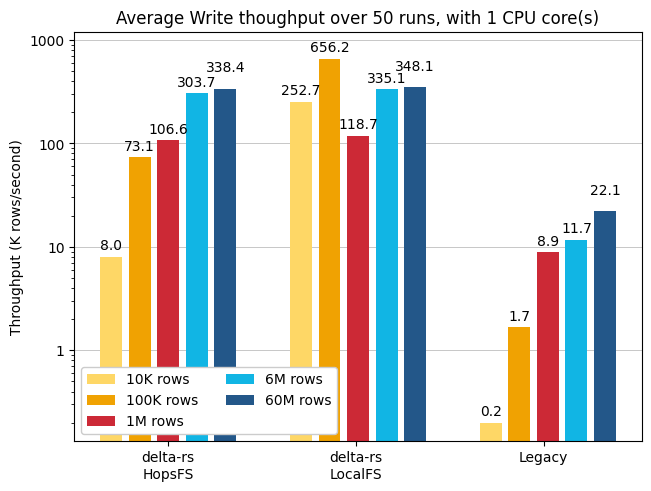
\includegraphics[width=\textwidth]{figures/5-results/write/write_throughput_1_core.png}
        \caption[Histogram of the write experiment - Throughput - 1 CPU core]{Histogram in log-scale of the write experiment results expressed as throughput. The experiment was performed with one \glstext{CPU} core.}
        \label{fig:res_write_throughput}
    \end{minipage}
\end{figure}

Figures~\ref{fig:res_write_time} and \ref{fig:res_write_throughput}, and Tables~\ref{tbl:res_write_time_cpu_perc} and \ref{tbl:res_write_throughput_cpu_perc} report the results of the write experiments performed. The results are expressed in latency in Figure~\ref{fig:res_write_time} and Table~\ref{tbl:res_write_time_cpu_perc}, and expressed in throughput in Figure~\ref{fig:res_write_throughput} and Table~\ref{tbl:res_write_throughput_cpu_perc}. The experiments were performed on the three systems defined in Section~\ref{subsec:experimental_design}. The five tables of different sizes being written were defined in Section~\ref{subsec:dataset}.

Both histograms, i.e., Figures~\ref{fig:res_write_time} and \ref{fig:res_write_throughput} report the results of the experiment performed with one \gls{CPU} core. On the other hand, the Tables~\ref{tbl:res_write_time_cpu_perc} and \ref{tbl:res_write_throughput_cpu_perc} on top of reporting the results of the one \gls{CPU} core experiment also present a calculated percentage of improvement (decrease in the case of latency, increase in the case of throughput) of the metric as the \gls{CPU} cores increase.

\subsubsection*{delta-rs on \glsentryshort{HopsFS} vs. delta-rs on \glsentryshort{LocalFS}}

The latency measured using the delta-rs on \gls{LocalFS} pipeline is around ten times lower than the latency measured using the delta-rs on \gls{HopsFS} pipeline for small tables, i.e., 10K and 100K rows. On the other hand, the latency in the two pipelines has the same significant figure in experiments performed with larger tables, i.e., 1M, 10M, 6M, and 60M rows. Overall, the latency measured in the delta-rs on \gls{LocalFS} pipeline remains lower in absolute terms than the latency measured using the delta-rs on \gls{HopsFS} pipeline in all experiments.

\subsubsection*{delta-rs on \glsentryshort{HopsFS} vs. Legacy pipeline}

The latency measured using the delta-rs on \gls{HopsFS} pipeline results more than ten times lower than the latency measured using the Legacy pipeline in all experiments. This trend is more prominent for smaller tables (10K and 100K rows) where latency measured using the delta-rs on \gls{HopsFS} pipeline is forty times lower than the latency measured using the Legacy pipeline. The tendency is less marked for larger tables (6M and 60M rows) where latency measured using the delta-rs on \gls{HopsFS} pipeline is around twenty times lower than the latency measured using the Legacy pipeline.

\subsubsection*{Change of performance as the \glsentryshort{CPU} cores increase}

During experiments with more \gls{CPU} cores, in delta-rs based pipelines (writing on \gls{HopsFS} or \gls{LocalFS}) the latency during write operation decreases by a considerable amount: 20-30\%, only when writing larger tables (6M and 60M rows), while it decreases by a lower margin: 5-10\% on smaller tables (100K and 1M rows), even slightly increasing on the smallest table (10K rows). It should be noted that latency decreases as described in the two \gls{CPU} cores experiments, remaining on similar improvements even with more \gls{CPU} cores.

Considering the Legacy pipeline, experiments with more \gls{CPU} cores did not decrease the latency by more than 7\% except for the largest table (60M rows). This table benefitted from a latency decrease of around 14\%. The smallest tables (10K and 100K) reported slight increases in the measured latency.

\subsection{Read Experiments}

\begin{figure}
    \centering
    \begin{minipage}[b]{\textwidth}
        \captionof{table}[Read experiments results expressed as latency]{Read experiment results expressed as latency. Experiments performed with more than one \glstext{CPU} core are expressed as latency percentage decrease compared to the one \glstext{CPU} core experiment.}
        \label{tbl:res_read_time_cpu_perc}
        \begin{tabular}{c r S[table-format=4.5] S[table-format=2.2] S[table-format=2.2] S[table-format=2.2]} 
            \toprule
            Pipeline\Tstrut\Bstrut & {\thead{Number\\ of rows}} & {\thead{1 CPU core latency \\ (seconds)}} & {\thead{2 CPU cores\\ (\% decrease)}} & {\thead{4 CPU cores\\ (\% decrease)}} & {\thead{8 CPU cores\\ (\% decrease)}} \\
            \midrule
            \multirow{5}{4em}{delta-rs\\ HopsFS} & 10K & 0.05342 & 22.65 & 18.84 & 18.95\\ 
            & 100K & 0.05757 & 1.15 & 3.76 & 5.19\\ 
            & 1M & 0.53855 & 56.53 & 65.00 & 67.71\\
            & 6M & 1.94899 & 53.40 & 72.74 & 74.48\\
            & 60M & 22.98065 & 50.34 & 75.72 & 87.20\\
            \midrule
            \multirow{5}{4em}{delta-rs\\ LocalFS} & 10K & 0.00419 & 31.48 & 35.91 & 29.66\\ 
            & 100K & 0.02696 & 51.54 & 65.76 & 64.84\\ 
            & 1M &   0.42009 & 52.45 & 78.64 & 89.75\\
            & 6M &   1.68223 & 55.56 & 77.99 & 89.57\\
            & 60M &  19.56547 & 51.72 & 75.41 & 88.32\\
            \midrule
            \multirow{5}{4em}{Legacy} & 10K & 0.63159 & 1.06 & -0.67 & 0.67\\ 
            & 100K & 2.65010 & -0.50 & 0.39 & -0.46\\ 
            & 1M &   8.59636 & -0.24 & -1.81 & 2.89\\
            & 6M &   33.52964 & 0.46 & 0.23 & 0.30\\
            & 60M &  33.69772 & 0.16 & 0.13 & 1.64\\
            \bottomrule
        \end{tabular}
    \end{minipage}
    \begin{minipage}[b]{\textwidth}
        \includegraphics[width=\textwidth]{figures/5-results/read/read_time_1_core.png}
        \caption[Histogram of the read experiment - Latency - 1 CPU core]{Histogram in log-scale of the read experiment results expressed as latency. The experiment was performed with one \glstext{CPU} core.}
        \label{fig:res_read_time}
    \end{minipage}
\end{figure}

\begin{figure}
    \centering
    \begin{minipage}[b]{\textwidth}
        \captionof{table}[Read experiments results expressed as throughput]{Read experiment results expressed as throughput. Experiments performed with more than one \glstext{CPU} core are expressed as throughput percentage increase compared to the one \glstext{CPU} core experiment.}
        \label{tbl:res_read_throughput_cpu_perc}
        \begin{tabular}{c r S[table-format=4.5] S[table-format=2.2] S[table-format=2.2] S[table-format=2.2]}
            \toprule
            Pipeline\Tstrut\Bstrut & {\thead{Number\\ of rows}} & {\thead{1 CPU core throughput \\ (k rows/second)}} & {\thead{2 CPU cores\\ (\% increase)}} & {\thead{4 CPU cores\\ (\% increase)}} & {\thead{8 CPU cores\\ (\% increase)}} \\
            \midrule
            \multirow{5}{4em}{delta-rs\\ HopsFS} & 10K & 187.16853 & 29.28 & 23.21 & 23.38\\ 
            & 100K & 1736.90799 & 1.17 & 3.90 & 5.48\\ 
            & 1M &   1856.83167 & 130.02 & 185.74 & 209.69\\
            & 6M &   3078.51299 & 114.57 & 266.87 & 291.92\\
            & 60M &  2610.89146 & 101.35 & 311.83 & 681.03\\
            \midrule
            \multirow{5}{4em}{delta-rs\\ LocalFS} & 10K & 2384.58699 & 45.94 & 56.04 & 42.18\\ 
            & 100K & 3708.25787 & 106.37 & 192.07 & 184.38\\ 
            & 1M &   2380.40381 & 110.28 & 368.24 & 875.15\\
            & 6M &   3566.67454 & 125.01 & 354.40 & 858.64\\
            & 60M &  3066.62644 & 107.11 & 306.75 & 756.07\\
            \midrule
            \multirow{5}{4em}{Legacy} & 10K & 15.83285 & 1.07 & -0.67 & 0.67\\ 
            & 100K & 37.73432 & -0.50 & 0.39 & -0.45\\ 
            & 1M &   116.32820 & -0.24 & -1.78 & 2.98\\
            & 6M &   178.94612 & 0.46 & 0.23 & 0.30\\
            & 60M &  1780.53563 & 0.16 & 0.13 & 1.67\\
            \bottomrule
        \end{tabular}
    \end{minipage}
    \begin{minipage}[b]{\textwidth}
        \includegraphics[width=\textwidth]{figures/5-results/read/read_throughput_1_core.png}
        \caption[Histogram of the read experiment - Throughput - 1 CPU core]{Histogram in log-scale of the read experiment results expressed as throughput. The experiment was performed with one \glstext{CPU} core.}
        \label{fig:res_read_throughput}
    \end{minipage}
\end{figure}

Figures~\ref{fig:res_read_time} and \ref{fig:res_read_throughput}, and Tables~\ref{tbl:res_write_time_cpu_perc} and \ref{tbl:res_read_throughput_cpu_perc} report the results of the read experiments performed. The results are expressed in latency in Figure~\ref{fig:res_read_time} and Table~\ref{tbl:res_read_time_cpu_perc}, and expressed in throughput in Figure~\ref{fig:res_read_throughput} and Table~\ref{tbl:res_read_throughput_cpu_perc}. The experiments were performed on the three systems defined in Section~\ref{subsec:experimental_design}. The five tables of different sizes being written were defined in Section~\ref{subsec:dataset}.

Both histograms, i.e., Figures~\ref{fig:res_read_time} and \ref{fig:res_read_throughput} report the results of the experiment performed with one \gls{CPU} core. On the other hand, the Tables~\ref{tbl:res_read_time_cpu_perc} and \ref{tbl:res_read_throughput_cpu_perc} on top of reporting the results of the one \gls{CPU} core experiment also present a calculated percentage of improvement (decrease in the case of latency, increase in the case of throughput) of the metric as the \gls{CPU} cores increase.

\subsubsection*{delta-rs on \glsentryshort{HopsFS} vs. delta-rs on \glsentryshort{LocalFS}}

The latency measured using the delta-rs on \gls{LocalFS} pipeline is around ten times lower than the latency measured using the delta-rs on \gls{HopsFS} pipeline in the experiment with the smallest table, i.e., 10K rows. On the other hand, the latency in the two pipelines has the same significant figure on experiments performed with larger tables, i.e., 100K, 1M, 10M, 6M, and 60M rows. Overall, the latency measured in the delta-rs on \gls{LocalFS} pipeline remains lower in absolute terms than the latency measured using the delta-rs on \gls{HopsFS} pipeline in all experiments.

\subsubsection*{delta-rs on \glsentryshort{HopsFS} vs. Legacy pipeline}

The latency measured using the delta-rs on \gls{HopsFS} pipeline results from 47\% up to forty times lower than the latency measured using the Legacy pipeline. The largest latency reduction compared to the legacy system (forty times) is obtained with the 100K rows table. In contrast, the smallest decrease in latency between newer and older systems is obtained with the largest table, i.e., 60M rows. For all other tables, the delta-rs on \gls{HopsFS} pipeline has around ten times lower latency than the legacy system.

\subsubsection*{Change of performance as the \glsentryshort{CPU} cores increase}

During experiments with more \gls{CPU} cores, in delta-rs based pipelines (reading on \gls{HopsFS} or \gls{LocalFS}), the latency during read operation decreases by a considerable amount: +50\%, when reading larger tables (1M, 6M and 60M rows), while it decreases by a lower margin: 20-30\% on smaller tables, i.e., 10K and 100K rows. It should be noted that latency decreases in reads with larger tables (1M, 6M, and 60M rows) following an inverse linear relationship with the increase of \gls{CPU} cores: two \gls{CPU} cores, latency halves, four \gls{CPU} cores, latency quarters, eight \gls{CPU} cores, latency is decreased to an eighth. On the other hand, throughput follows a linear relationship with the increase of \gls{CPU} cores.

Considering the Legacy pipeline, experiments with more \gls{CPU} cores did not decrease the latency by more than 2\%. Histograms comparing the three pipelines look radically different in experiments with more \gls{CPU} cores due to how delta-rs scales with the increase of \gls{CPU} cores. They can be accessed in the Appendix \ref{appx:res_write}.

\subsection{Legacy pipeline write latency breakdown}

\begin{figure}
    \centering
    \begin{minipage}[b]{\textwidth}
        \captionof{table}[Writes on legacy pipeline - Time breakdown]{Contributions to the write latency of the upload and materialization steps in the legacy pipeline. Experiments performed with more than one \glstext{CPU} core are expressed as latency percentage decrease compared to the one \glstext{CPU} core experiment.}
        \label{tbl:hudi_virtualiz_breakdown_cpu_perc}
        \begin{tabular}{r S[table-format=4.2] S[table-format=4.2] S[table-format=2.2] S[table-format=2.2] S[table-format=2.2] S[table-format=2.2] S[table-format=2.2] S[table-format=2.2]} 
            \toprule
            \multirow{2}{*}{{\thead{Number\\ of rows}}} & \multicolumn{2}{c}{{\thead{1 CPU core\\ latency (seconds)}}} & \multicolumn{2}{c}{{\thead{2 CPU cores\\ (\% decrease)}}} & \multicolumn{2}{c}{{\thead{4 CPU cores\\ (\% decrease)}}} & \multicolumn{2}{c}{{\thead{8 CPU cores\\ (\% decrease)}}}\\
            & {upl.} & {mat.} & {upl.} & {mat.} & {upl.} & {mat.} & {upl.} & {mat.}\\
            \midrule
            10K &  2.48 & 47.72 & 3.99 & -1.27 & 4.10 & -2.47 & 4.22 & -2.35\\
            100K & 3.66 & 55.90 & 6.37 & -0.78 & 5.55 & -0.27 & 6.25 & -1.69\\
            1M   & 22.59 & 89.57 & 17.52 & -0.39 & 14.89 & -0.01 & 16.51 & -1.05\\
            6M   & 244.61 & 267.24 & 15.83 & -0.10 & 13.46 & -1.15 & 15.10 & -0.38\\
            60M &  2437.78 & 278.05 & 15.33 & 0.39 & 15.15 & 0.16 & 15.94 & 0.82\\
            \bottomrule
        \end{tabular}
    \end{minipage}
    \begin{minipage}[b]{\textwidth}
        \includegraphics[width=\textwidth]{figures/5-results/hudi_virtualiz_1_core.png}
        \caption[Histogram of the write on legacy pipeline - Time breakdown - 1 core]{Histogram in log-scale displaying the contributions to the write latency of the upload and materialization steps in the legacy pipeline. The experiment was performed with one \glstext{CPU} core.}
        \label{fig:hudi_virtualiz_breakdown}
    \end{minipage}
\end{figure}

Table \ref{tbl:hudi_virtualiz_breakdown_cpu_perc} and Figure \ref{fig:hudi_virtualiz_breakdown} show the write latency breakdown of the Legacy pipeline into upload time and materialization time, the different steps of the Legacy pipeline as explained in Section \ref{subsec:legacy_sys_writing}. The breakdown is proposed for all five tables defined in Section \ref{subsec:dataset}. Figure \ref{fig:hudi_virtualiz_breakdown} reports the data from the one \gls{CPU} core experiment. In contrast, Table \ref{tbl:hudi_virtualiz_breakdown_cpu_perc} reports both the one \gls{CPU} core experiment data and also a calculated percentage of improvement, i.e., decrease, of the latency as the \gls{CPU} cores increase.

Considering the upload time contribution to the write latency, this represents a small percentage (around 5\%) when writing smaller tables, i.e., 10K and 100K rows. Nonetheless, the upload contribution grows following a similarly linear pattern in larger tables, i.e., between 100K and 60M rows. This radically changes the proportion between the upload and materialized contribution to the write latency, making the upload time 90\% of the total write latency for the 60M rows table. On the other hand, the materialization time contribution, while starting with high latency contribution (95\% of the total), its absolute value does not increase by more than a significant figure even if the table size increased by three significant figures.

Observing the results of experiments using more \gls{CPU} cores, the upload time benefits from a higher number of \gls{CPU} cores, in particular with larger tables (15\% latency decrease) and less with smaller tables (4\% latency decrease). On the other hand, the materialize time does not improve performance, having either small decreases in latency or small increases (both around 1-2\%).

\subsection{In-memory resources usage}
\label{subsec:resources_usage}

The experimental environment resources defined in Section \ref{subsec:exp_env} were adjusted according to the computational needs. In particular, write operations were demanding on the available \gls{RAM} resources, requiring up to 24 GBs to operate with the larger tables (6M and 60M rows). The system was adjusted to allocate 32768 MB of \gls{RAM} to avoid slowing down operations.

\section{Results analysis and discussion}
    \label{sec:res_analysis_discuss}
    This section complements the results section by analyzing the results shown in Section \ref{sec:major_res} one by one.

\subsection{Write operations using delta-rs are up to 40 times faster than the legacy Spark pipeline}
The writing experiment reveals that the use of the delta-rs library achieves up to 40 times the performance of the Legacy Spark pipeline with smaller tables (10K and 100K rows). The delta-rs pipelines (both on \gls{HopsFS} and on \gls{LocalFS}) achieve higher performances even with bigger tables (1M, 6M, and 60M rows), but with lower rates (15-26 times better). 

This experimental result shows that a Rust pipeline writing data on Delta Lake tables is indeed faster than the legacy Spark pipeline in all writing tests. The rate of this improvement varies (40 times better vs. 15.35 times better when comparing 10K and 60M rows) and it is decreasing with the size of the table. This suggests that a writing a larger table (more than 60M rows) the Legacy Spark pipeline performs better than the delta-rs pipelines. This insight can be verified with further experiments using larger tables (more than 60M rows).

\subsection{Read operations using delta-rs are increasingly faster than the legacy Spark pipeline}

The reading experiment reveals that delta-rs pipelines achieve increasingly better performance as the size of the table grows. The throughput in the delta-rs on \gls{HopsFS} is up to 3 significant figures greater than the throughput of the legacy Spark pipeline.

This experiment results show that a Rust pipeline reading data on Delta Lake tables is indeed faster than the legacy Spark pipeline. Moreover, contrary to what was suggested in the introduction, i.e. that a Spark-based pipeline would have faster performance as the size of the table increases, this is not the case with the analyzed experiments, where the difference in proportion between the two pipelines grows significantly as the table sizes increase (20 times better vs. 1000+ times better when comparing 10K and 60M rows).

\subsection{Increasing the CPU cores does not increase the read or write performance dramatically}

The experiments run with more \gls{CPU} cores reveal that even if the computational resources increase the throughput does not increase linearly, e.g. no experiment run with 2 \gls{CPU} cores achieved more than a 33\% throughput increase. Moreover, reading experiments did not see major improvements (more than 20\%) in throughput except the experiments performed with delta-rs on the \gls{LocalFS}. On the other hand, writing experiments did show improvements in throughput, even if limited if compared to the increase in computing power, e.g. the best results were achieved with larger tables where adding a single core resulted in a 32.89\% improvement, but this is limited if the fact that computing resources were doubled is considered.

\subsection{The upload time in the legacy Spark pipeline becomes the bottleneck as table size increases}

In the writing experiment on the legacy Spark pipeline, as explained in Section \todo[inline]{Ref here time breakdown expel.}, writing time can be broken down into two upload and materialization time. This experiment reveals that as the table size increases, the contribution of the upload time drastically changes (4.96\% vs. 89.76\% contribution when comparing 10K and 60M rows tables). This suggests that the upload is the phase that limits the system to scale more efficiently, and thus has a higher throughput, as table size increases.

\cleardoublepage

\chapter{Conclusions and Future work}
    \label{ch:conclusions_and_future_work}
    This chapter presents the conclusions of the thesis work. It starts with Section \ref{sec:conclusions} that compares the experimental findings with the Research Question to outline this thesis contribution. Section \ref{sec:limitations} then explains the limitations of the project in terms of resources and scope. Finally, Section \ref{sec:future_work} complements the chapter by considering possible future work stemming from this thesis.

\section{Conclusions}
    \label{sec:conclusions}
    This thesis work posed two \glspl{RQ} defined in Section \ref{subsec:researchQuestion}. These were: 
\begin{enumerate}
    \item[RQ1:] How can we add support for \gls{HDFS} and \gls{HopsFS} to the delta-rs library?
    \item[RQ2:] What is the difference in latency and throughput between the current legacy system (Spark-based in writing) reading and writing to Apache Hudi compared to a delta-rs library-based reading and writing to Delta Lake, in \gls{HopsFS}?
\end{enumerate}
The work conducted in this thesis answered these two questions by performing a system implementation and then evaluating the newly implemented system. 

The first step was adding support for \gls{HopsFS} in the delta-rs library. This was achieved by modifying the hdfs-native \cite{binfordKimahrimanHdfsnative2024} library, which reimplements a \gls{HDFS} client in Rust. 

The second step was measuring and comparing the newly implemented system's performance with the legacy system. The metrics used were the latency (seconds) of the read and write operations and the throughput (rows/second), which was calculated by dividing the table size (in rows) by the latency of the operation. The results presented in Chapter \ref{ch:results_and_analysis} revealed that the delta-rs-based access to Delta Lake has a latency at least ten times lower in both read and write operations for tables from 10K to 6M rows in size. The write experiments show that the delta-rs library performs up to forty times better with smaller tables (10K and 100K) while still outperforming by ten times the legacy pipeline on the largest table (60M rows). This difference suggests that larger tables might have a threshold where a Spark-based system would perform better, but more experiments with larger tables are needed to verify the trend.
Similarly, in the reading experiments, delta-rs outperforms the legacy pipeline more with smaller tables (10K and 100K rows), even if only by a factor of fifteen instead of forty, as seen for the writing experiments. This is probably caused by using a Spark alternative in the legacy system's reading process (Arrow Flight and DuckDB), which already improves Spark performances on smaller tables. One last notable finding on the difference between the newly implemented system and the legacy pipeline is the difference in scalability as resources increase. Experiments were conducted with an increasing number of \gls{CPU} cores (from 1 to 8 \gls{CPU} cores), and the results showed that delta-rs, being a local process, is much more suited for making use of those resources with an up to 31\% reduction in latency during the writing and an 87\% reduction during reading.

Overall, the experiments' results recommend the adoption of the newly implemented system in the defined use case (Section \ref{subsec:use_case}), either as a replacement or an alternative for users who wish to store data in a Delta Table within the Offline Feature Store.


\section{Limitations}
    \label{sec:limitations}
    The limitations of this study mostly derive from the constraints of resources, in terms of time and computational resources, and scope, which is mainly linked to the defined use case (Section~\ref{subsec:use_case}). 

This project's scope is to improve the latency of the Hopsworks offline feature store, and this is the technology on which the implementation and the experiments were based. This outlines the limited generalization of the results obtained, which are biased from the use of technology in collaboration with the company developing it. Additionally, a specific use case was defined (Section~\ref{subsec:use_case}) to choose the \gls{CPU} loads and data loads on which the experiments would be conducted. This helps to define a perimeter of the thesis contribution but also limits the thesis impact on this specific use case, requiring more research to verify the same hypothesis in a different scenario.

While great in size, the computational resources provided were used in a shared environment that could only be used for a limited amount of time and only if it was not operating other, more critical workloads. Time also played a role in limiting the number of experiments to calculate a 95\% confidence interval. All experiments were run fifty times, which significantly increased the time required to perform all experiments. 

\section{Future work}
    \label{sec:future_work}
    The results and limitations of this thesis offer a good starting point for future work. As outlined in the limitations section before, this thesis's scope and resources were limited. Conducting new experiments on the system performance by relaxing one or more constraints could bring new results that can be more general.

Considering the system research contribution of this thesis, this could be expanded mostly for Hopsworks \gls{AB} needs as the code works with key components of their infrastructure, e.g. \gls{HopsFS}, that while open-source are not used much outside the company. The code is unlikely to see use in the delta-rs library, as even if this is a solid contribution, it only fits a single company's use case, and it is very limited in their applications outside it. Future system contributions could still use the code developed in this thesis as a baseline to be compared with new delta-rs implementations or other ways to read and write on an Offline Feature Store.

The future work that could be carried out on the system evaluation could expand on one or more of these aspects: data, pipelines, and experimental environment. Expanding on data would mean running the experiments with larger tables (600M rows, 6BN rows, etc.) to explore and verify if a threshold where a Spark-based system performs better than delta-rs is present and at which table size. Also, making variations on the data sources would be a valid approach, although this would make this thesis an invalid baseline. The pipelines that were defined are specific to delta-rs or the Hopsworks architecture. Verifying the speed of other Offline Feature Stores as Databricks' would help generalize the results on a broader area. This would help clear out which approach performs best (between Spark and delta-rs) across different systems.
The experimental environment as said in the limitations, was a shared environment with large resources, but varying on the current machine usage by other company's employees. Using clean isolated hardware could help future research verify this thesis's findings, isolating the variable results of a shared environment.

%%%%%%%%%%%%%%%%%%%%%%%%%%%%%%%%%%%%%%%%%%%%%%%%%%%%%%%%%%%%%%%%%%%%%%%%%%%%%%%%%%%%%%%%
%%                                 REFERENCES
%%%%%%%%%%%%%%%%%%%%%%%%%%%%%%%%%%%%%%%%%%%%%%%%%%%%%%%%%%%%%%%%%%%%%%%%%%%%%%%%%%%%%%%%
%\noindent\rule{\textwidth}{0.4mm}
%%\engExpl{In the references, let Zotero or other tool fill this in for you. I suggest an extended version of the IEEE style, to include URLs, DOIs, ISBNs, etc., to make it easier for your reader to find them. This will make life easier for your opponents and examiner. \\IEEE Editorial Style Manual: \url{https://www.ieee.org/content/dam/ieee-org/ieee/web/org/conferences/style_references_manual.pdf}}

\cleardoublepage

% Print the bibliography (and make it appear in the table of contents)
\renewcommand{\bibname}{References}

\ifbiblatex
    %\typeout{Biblatex current language is \currentlang}
    \printbibliography[heading=bibintoc]
\else
    \phantomsection  % make it include a hyperref - see https://tex.stackexchange.com/a/98995
    \addcontentsline{toc}{chapter}{References}
    \bibliography{references}
\fi

%%%%%%%%%%%%%%%%%%%%%%%%%%%%%%%%%%%%%%%%%%%%%%%%%%%%%%%%%%%%%%%%%%%%%%%%%%%%%%%%%%%%%%%%
%%                                 APPENDIX
%%%%%%%%%%%%%%%%%%%%%%%%%%%%%%%%%%%%%%%%%%%%%%%%%%%%%%%%%%%%%%%%%%%%%%%%%%%%%%%%%%%%%%%%
%% If you do not have an appendix, do not include the \textbackslash cleardoublepage command below; otherwise, the last page number in the metadata will be one too large.}
\cleardoublepage

\appendix
\renewcommand{\chaptermark}[1]{\markboth{Appendix \thechapter\relax:\thinspace\relax#1}{}}

\chapter{System architectures}
    \label{appx:sys_arch}
    % Small appendix expl.
This appendix reports the legacy architecture diagrams shown in Section \ref{sec:arch_sys} increased in size to improve readability.

\begin{figure}
    \begin{center}
      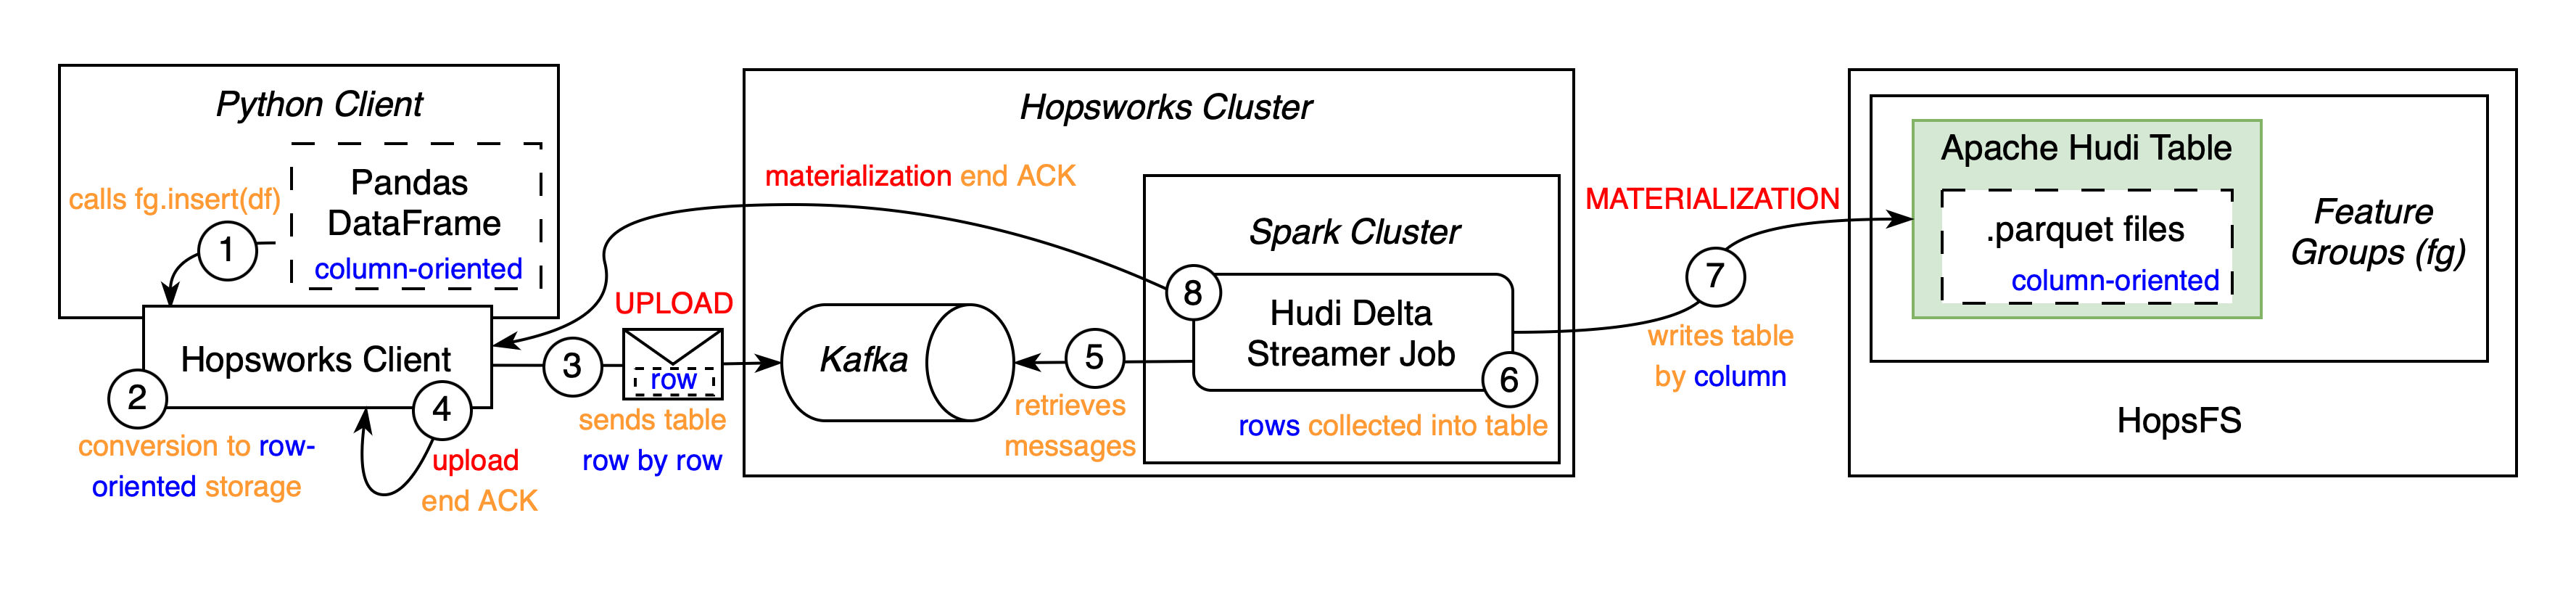
\includegraphics[angle=90,origin=c,keepaspectratio,height=12.5cm]{figures/2-background/FeatureStore-writing.png}
    \end{center}
    \caption[Legacy system - Write process - Magnified diagram]{Legacy system writing a Pandas data frame from a Python client to the Hopsworks offline Feature Store.  This image was magnified to enhance visualization.}
    \label{fig:appx_featurestore_writing}
\end{figure}

\begin{figure}
    \begin{center}
      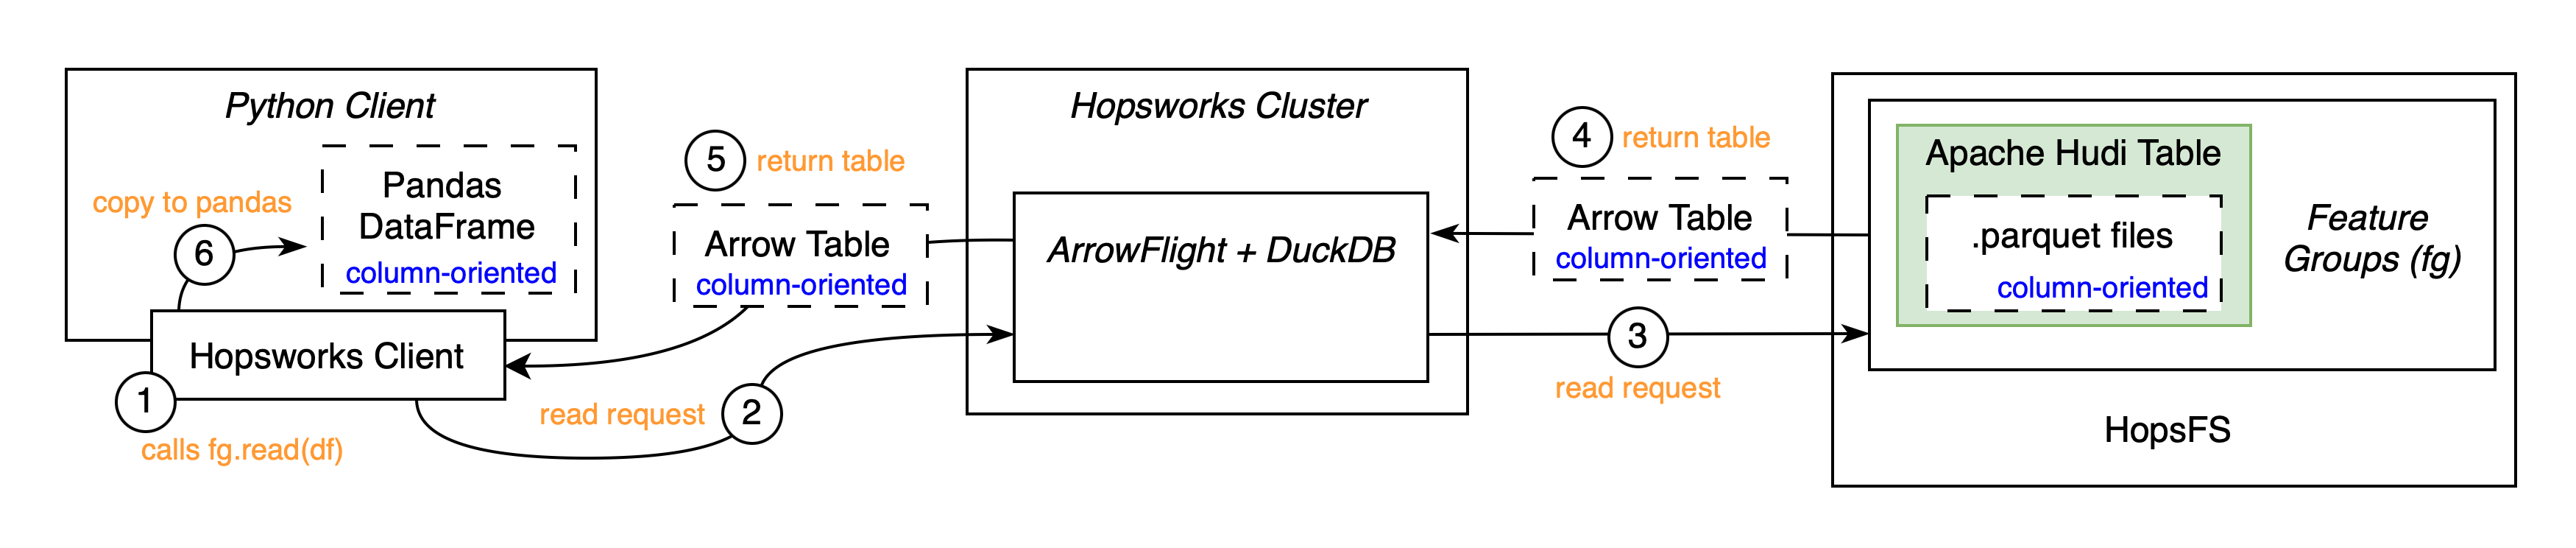
\includegraphics[angle=90,origin=c,keepaspectratio,height=12.5cm]{figures/2-background/FeatureStore-reading.png}
    \end{center}
    \caption[Legacy system - Read process - Magnified diagram]{Legacy system reading a table from the Hopsworks offline feature store and loading it into the Python client local memory. This image was magnified to enhance visualization.}
    \label{fig:appx_featurestore_reading}
\end{figure}

\chapter{Write experiments results}
    \label{appx:res_write}
    % Brief expl
This appendix reports all graphs and tables related to all the writing experiments conducted. Results are reported first expressed as latency (measured during the experiments), then as throughput (computed from the latency and table size).

%%%%%%%%%%%%%%%%%%%%%%%%%%%%%%%%%%%%%%%%%%%%%%%%%%%%%%%%%%%%%%%%%
%%%%%%%%%%%%              LATENCY             %%%%%%%%%%%%%%%%%%%
%%%%%%%%%%%%%%%%%%%%%%%%%%%%%%%%%%%%%%%%%%%%%%%%%%%%%%%%%%%%%%%%%
\begin{figure}
    \centering
    \begin{minipage}[b]{\textwidth}
        \centering
        \captionof{table}[Write experiment - Latency - 1 CPU core]{Write experiment results expressed as latency. The experiment was performed with one \glstext{CPU} core.}
        \label{tbl:appx_res_write_time_1_core}
        \begin{tabular}{c r S[table-format=5.5] S[table-format=5.5] S[table-format=5.5]} 
            \toprule
            \multirow{2}{*}{{Pipeline\Tstrut\Bstrut}} & \multirow{2}{*}{{\thead{Number\\ of rows}}} & {\multirow{2}{*}{{\thead{Latency \\ (seconds)}}}} & \multicolumn{2}{c}{{\thead{Latency (seconds) \\95\% Confidence Interval}}}\\
                                                      &                                             &                                                   & {low} & {high}\\
            \midrule
            \multirow{5}{4em}{delta-rs\\ HopsFS} & 10K  &    1.25088 &    1.23807 &   1.26545\\ 
                                                 & 100K &    1.36828 &    1.33757 &   1.38982\\ 
                                                 & 1M   &    9.38152 &    9.23971 &   9.52904\\
                                                 & 6M   &   19.75469 &   19.33270 &  20.11785\\
                                                 & 60M  &  177.30707 &  174.62871 & 180.01732\\
            \midrule
            \multirow{5}{4em}{delta-rs\\ LocalFS} & 10K  &    0.03957 &   0.03770 &   0.04153\\ 
                                                  & 100K &    0.15240 &   0.14598 &   0.15888\\ 
                                                  & 1M   &    8.42252 &   8.28396 &   8.56376\\
                                                  & 6M   &   17.90634 &  17.48040 &  18.33585\\
                                                  & 60M  &  172.34552 & 169.74808 & 174.73138\\
            \midrule
            \multirow{5}{4em}{Legacy} & 10K  &    50.22767 &   49.53501 &   50.93664\\ 
                                      & 100K &    59.56187 &   58.89466 &   60.18496\\ 
                                      & 1M   &   112.19048 &  111.37162 &  113.00915\\
                                      & 6M   &   511.81693 &  510.75113 &  512.83672\\
                                      & 60M  &  2715.77285 & 2699.88061 & 2731.95225\\
            \bottomrule
        \end{tabular}
    \end{minipage}
    \begin{minipage}[b]{\textwidth}
        \centering
        \includegraphics[width=\textwidth]{figures/99-appendix/results-diagrams/write/write_time_1_core.png}
        \caption[Histogram of the write experiment - Latency - 1 CPU core]{Histogram in log-scale of the write experiment results expressed as latency. The experiment was performed with one \glstext{CPU} core.}
        \label{fig:appx_res_write_time_1_core}
    \end{minipage}
\end{figure}

\begin{figure}
    \centering
    \begin{minipage}[b]{\textwidth}
        \centering
        \captionof{table}[Write experiment - Latency - 2 CPU cores]{Write experiment results expressed as latency. The experiment was performed with two \glstext{CPU} cores.}
        \label{tbl:appx_res_write_time_2_cores}
        \begin{tabular}{c r S[table-format=5.5] S[table-format=5.5] S[table-format=5.5]} 
            \toprule
            \multirow{2}{*}{{Pipeline\Tstrut\Bstrut}} & \multirow{2}{*}{{\thead{Number\\ of rows}}} & {\multirow{2}{*}{{\thead{Latency \\ (seconds)}}}} & \multicolumn{2}{c}{{\thead{Latency (seconds) \\95\% Confidence Interval}}}\\
                                                      &                                             &                                                   & {low} & {high}\\
            \midrule
            \multirow{5}{4em}{delta-rs\\ HopsFS} & 10K  &    1.26239 &    1.25079 &   1.27639\\ 
                                                 & 100K &    1.30812 &    1.28050 &   1.33217\\ 
                                                 & 1M   &    8.51536 &    8.34333 &   8.70077\\
                                                 & 6M   &   16.29042 &   15.90659 &  16.67362\\
                                                 & 60M  &  134.06089 &  131.65031 & 136.39761\\
            \midrule
            \multirow{5}{4em}{delta-rs\\ LocalFS} & 10K  &    0.04823 &   0.04640 &   0.04997\\ 
                                                  & 100K &    0.13714 &   0.13402 &   0.14050\\ 
                                                  & 1M   &    7.18530 &   7.03747 &   7.35128\\
                                                  & 6M   &   15.26632 &  14.85172 &  15.65167\\
                                                  & 60M  &  129.82007 & 127.60020 & 132.04689\\
            \midrule
            \multirow{5}{4em}{Legacy} & 10K  &    50.72405 &   50.10769 &   51.30686\\ 
                                      & 100K &    59.78810 &   58.97997 &   60.47427\\ 
                                      & 1M   &   108.56499 &  108.01124 &  109.08128\\
                                      & 6M   &   473.37954 &  472.34534 &  474.43740\\
                                      & 60M  &  2340.77013 & 2333.99443 & 2347.97127\\
            \bottomrule
        \end{tabular}
    \end{minipage}
    \begin{minipage}[b]{\textwidth}
        \centering
        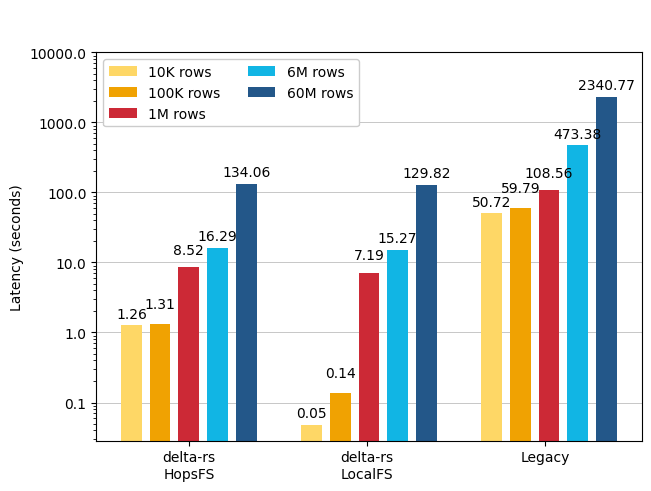
\includegraphics[width=\textwidth]{figures/99-appendix/results-diagrams/write/write_time_2_core.png}
        \caption[Histogram of the write experiment - Latency - 2 CPU cores]{Histogram in log-scale of the write experiment results expressed as latency. The experiment was performed with two \glstext{CPU} cores.}
        \label{fig:appx_res_write_time_2_cores}
    \end{minipage}
\end{figure}

\begin{figure}
    \centering
    \begin{minipage}[b]{\textwidth}
        \centering
        \captionof{table}[Write experiment - Latency - 4 CPU cores]{Write experiment results expressed as latency. The experiment was performed with four \glstext{CPU} cores.}
        \label{tbl:appx_res_write_time_4_cores}
        \begin{tabular}{c r S[table-format=5.5] S[table-format=5.5] S[table-format=5.5]} 
            \toprule
            \multirow{2}{*}{{Pipeline\Tstrut\Bstrut}} & \multirow{2}{*}{{\thead{Number\\ of rows}}} & {\multirow{2}{*}{{\thead{Latency \\ (seconds)}}}} & \multicolumn{2}{c}{{\thead{Latency (seconds) \\95\% Confidence Interval}}}\\
                                                      &                                             &                                                   & {low} & {high}\\
            \midrule
            \multirow{5}{4em}{delta-rs\\ HopsFS} & 10K  &    1.21642 &    1.20232 &   1.23231\\ 
                                                 & 100K &    1.33622 &    1.32294 &   1.34942\\ 
                                                 & 1M   &    8.41325 &    8.24770 &   8.58272\\
                                                 & 6M   &   16.22402 &   15.87946 &  16.59586\\
                                                 & 60M  &  124.10242 &  121.57723 & 126.81530\\
            \midrule
            \multirow{5}{4em}{delta-rs\\ LocalFS} & 10K  &    0.04572 &   0.04341 &   0.04807\\ 
                                                  & 100K &    0.13176 &   0.12880 &   0.13499\\ 
                                                  & 1M   &    7.18574 &   7.00679 &   7.36343\\
                                                  & 6M   &   14.55578 &  14.17679 &  14.94192\\
                                                  & 60M  &  121.37623 & 119.17256 & 123.69890\\
            \midrule
            \multirow{5}{4em}{Legacy} & 10K  &    51.28465 &   50.62282 &   51.90367\\ 
                                      & 100K &    59.52655 &   58.90537 &   60.15322\\ 
                                      & 1M   &   108.81674 &  108.25217 &  109.34234\\
                                      & 6M   &   481.98353 &  481.04435 &  482.92992\\
                                      & 60M  &  2346.04687 & 2336.99396 & 2355.19897\\
            \bottomrule
        \end{tabular}
    \end{minipage}
    \begin{minipage}[b]{\textwidth}
        \centering
        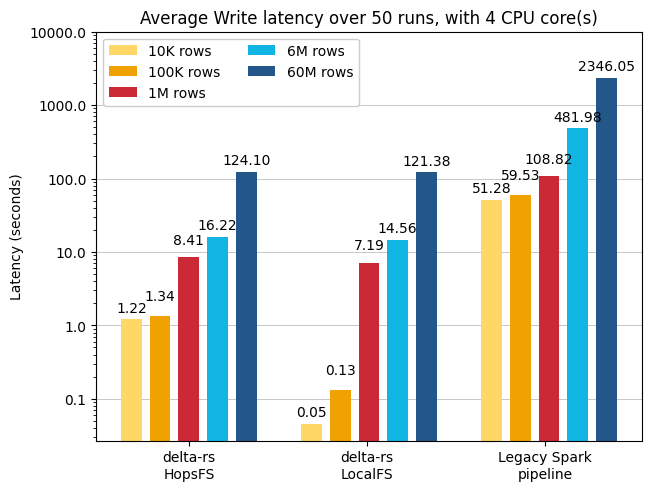
\includegraphics[width=\textwidth]{figures/99-appendix/results-diagrams/write/write_time_4_core.png}
        \caption[Histogram of the write experiment - Latency - 4 CPU cores]{Histogram in log-scale of the write experiment results expressed as latency. The experiment was performed with four \glstext{CPU} cores.}
        \label{fig:appx_res_write_time_4_cores}
    \end{minipage}
\end{figure}

\begin{figure}
    \centering
    \begin{minipage}[b]{\textwidth}
        \centering
        \captionof{table}[Write experiment - Latency - 8 CPU cores]{Write experiment results expressed as latency. The experiment was performed with eight \glstext{CPU} cores.}
        \label{tbl:appx_res_write_time_8_cores}
        \begin{tabular}{c r S[table-format=5.5] S[table-format=5.5] S[table-format=5.5]} 
            \toprule
            \multirow{2}{*}{{Pipeline\Tstrut\Bstrut}} & \multirow{2}{*}{{\thead{Number\\ of rows}}} & {\multirow{2}{*}{{\thead{Latency \\ (seconds)}}}} & \multicolumn{2}{c}{{\thead{Latency (seconds) \\95\% Confidence Interval}}}\\
                                                      &                                             &                                                   & {low} & {high}\\
            \midrule
            \multirow{5}{4em}{delta-rs\\ HopsFS} & 10K  &    1.36756 &    1.24934 &   1.57224\\ 
                                                 & 100K &    1.29243 &    1.26548 &   1.31099\\ 
                                                 & 1M   &    8.30120 &    8.14918 &   8.47040\\
                                                 & 6M   &   15.73847 &   15.28974 &  16.16084\\
                                                 & 60M  &  121.95014 &  119.59376 & 124.18097\\
            \midrule
            \multirow{5}{4em}{delta-rs\\ LocalFS} & 10K  &    0.04402 &   0.04174 &   0.04640\\ 
                                                  & 100K &    0.13648 &   0.13281 &   0.14061\\ 
                                                  & 1M   &    7.22872 &   7.07511 &   7.39893\\
                                                  & 6M   &   14.28157 &  13.90508 &  14.66126\\
                                                  & 60M  &  119.97915 & 117.76416 & 122.20882\\
            \midrule
            \multirow{5}{4em}{Legacy} & 10K  &    51.22859 &   50.59478 &   51.86476\\ 
                                      & 100K &    60.27751 &   59.72907 &   60.77130\\ 
                                      & 1M   &   109.38189 &  108.86830 &  109.88263\\
                                      & 6M   &   475.94345 &  474.83993 &  477.05274\\
                                      & 60M  &  2324.97917 & 2319.04203 & 2331.04794\\
            \bottomrule
        \end{tabular}
    \end{minipage}
    \begin{minipage}[b]{\textwidth}
        \centering
        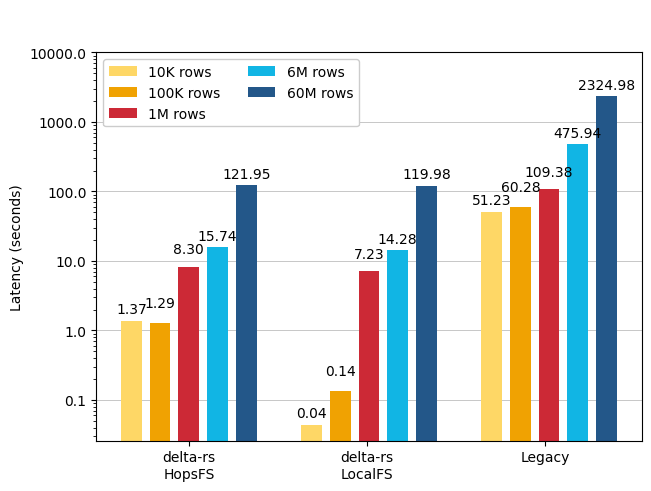
\includegraphics[width=\textwidth]{figures/99-appendix/results-diagrams/write/write_time_8_core.png}
        \caption[Histogram of the write experiment - Latency - 8 CPU cores]{Histogram in log-scale of the write experiment results expressed as latency. The experiment was performed with eight \glstext{CPU} cores.}
        \label{fig:appx_res_write_time_8_cores}
    \end{minipage}
\end{figure}

%%%%%%%%%%%%%%%%%%%%%%%%%%%%%%%%%%%%%%%%%%%%%%%%%%%%%%%%%%%%%%%%%
%%%%%%%%%%%%             THROUGHPUT           %%%%%%%%%%%%%%%%%%%
%%%%%%%%%%%%%%%%%%%%%%%%%%%%%%%%%%%%%%%%%%%%%%%%%%%%%%%%%%%%%%%%%

\begin{figure}
    \centering
    \begin{minipage}[b]{\textwidth}
        \centering
        \captionof{table}[Write experiment - Throughput - 1 CPU core]{Write experiment results expressed as throughput. The experiment was performed with one \glstext{CPU} core.}
        \label{tbl:appx_res_write_throughput_1_core}
        \begin{tabular}{c r S[table-format=5.5] S[table-format=5.5] S[table-format=5.5]} 
            \toprule
            \multirow{2}{*}{{Pipeline\Tstrut\Bstrut}} & \multirow{2}{*}{{\thead{Number\\ of rows}}} & {\multirow{2}{*}{{\thead{Throughput \\ (k rows/second)}}}} & \multicolumn{2}{c}{{\thead{Throughput (k rows/second) \\95\% Confidence Interval}}}\\
                                                      &                                             &                                                          & {low} & {high}\\
            \midrule
            \multirow{5}{4em}{delta-rs\\ HopsFS} & 10K  &    7.99436 &    7.90230 &   8.07705\\ 
                                                 & 100K &    7.30843 &    7.19514 &   7.47621\\ 
                                                 & 1M   &  106.59242 &  104.94226 & 108.22850\\
                                                 & 6M   &  303.72533 &  298.24252 & 310.35491\\
                                                 & 60M  &  338.39598 &  333.30126 & 343.58610\\
            \midrule
            \multirow{5}{4em}{delta-rs\\ LocalFS} & 10K  &  252.68238 &  240.73405 &  265.18632\\ 
                                                  & 100K &  656.15739 &  629.36777 &  684.98518\\ 
                                                  & 1M   &  118.72919 &  116.77110 &  120.71514\\
                                                  & 6M   &  335.07675 &  327.22770 &  343.24143\\
                                                  & 60M  &  348.13784 &  343.38422 &  353.46496\\
            \midrule
            \multirow{5}{4em}{Legacy} & 10K  &     0.19909 &    0.19632 &    0.20187\\ 
                                      & 100K &     1.67892 &    1.66154 &    1.69794\\ 
                                      & 1M   &     8.91341 &    8.84884 &    8.97894\\
                                      & 6M   &    11.72294 &   11.69963 &   11.74740\\
                                      & 60M  &    22.09315 &   21.96231 &   22.22320\\
            \bottomrule
        \end{tabular}
    \end{minipage}
    \begin{minipage}[b]{\textwidth}
        \centering
        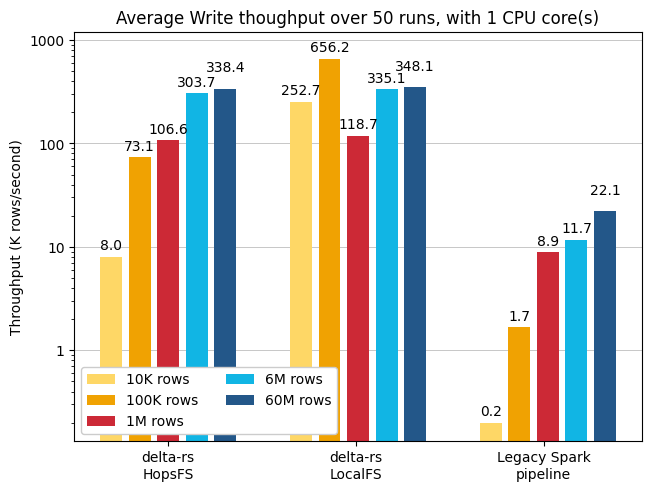
\includegraphics[width=\textwidth]{figures/99-appendix/results-diagrams/write/write_throughput_1_core.png}
        \caption[Histogram of the write experiment - Throughput - 1 CPU core]{Histogram in log-scale of the write experiment results expressed as throughput. The experiment was performed with one \glstext{CPU} core.}
        \label{fig:appx_res_write_throughput_1_core}
    \end{minipage}
\end{figure}

\begin{figure}
    \centering
    \begin{minipage}[b]{\textwidth}
        \centering
        \captionof{table}[Write experiment - Throughput - 2 CPU cores]{Write experiment results expressed as throughput. The experiment was performed with two \glstext{CPU} cores.}
        \label{tbl:appx_res_write_throughput_2_cores}
        \begin{tabular}{c r S[table-format=5.5] S[table-format=5.5] S[table-format=5.5]} 
            \toprule
            \multirow{2}{*}{{Pipeline\Tstrut\Bstrut}} & \multirow{2}{*}{{\thead{Number\\ of rows}}} & {\multirow{2}{*}{{\thead{Throughput \\ (k rows/second)}}}} & \multicolumn{2}{c}{{\thead{Throughput (k rows/second) \\95\% Confidence Interval}}}\\
                                                      &                                             &                                                          & {low} & {high}\\
            \midrule
            \multirow{5}{4em}{delta-rs\\ HopsFS} & 10K  &    7.92146 &    7.83458 &   7.99491\\ 
                                                 & 100K &   76.44507 &   75.06499 &  78.09433\\ 
                                                 & 1M   &  117.43478 &  114.93231 & 119.85614\\
                                                 & 6M   &  368.31440 &  359.84975 & 377.20198\\
                                                 & 60M  &  447.55780 &  439.89038 & 455.75281\\
            \midrule
            \multirow{5}{4em}{delta-rs\\ LocalFS} & 10K  &  207.31922 &  200.08626 &  215.49342\\ 
                                                  & 100K &  729.15967 &  711.73966 &  746.13854\\ 
                                                  & 1M   &  139.17297 &  136.03055 &  142.09647\\
                                                  & 6M   &  393.02185 &  383.34560 &  403.99352\\
                                                  & 60M  &  462.17814 &  454.38403 &  470.21868\\
            \midrule
            \multirow{5}{4em}{Legacy} & 10K  &     0.19714 &    0.19490 &    0.19957\\ 
                                      & 100K &     1.67257 &    1.65359 &    1.69549\\ 
                                      & 1M   &     9.21107 &    9.16747 &    9.25829\\
                                      & 6M   &    12.67481 &   12.64655 &   12.70257\\
                                      & 60M  &    25.63258 &   25.55397 &   25.70700\\
            \bottomrule
        \end{tabular}
    \end{minipage}
    \begin{minipage}[b]{\textwidth}
        \centering
        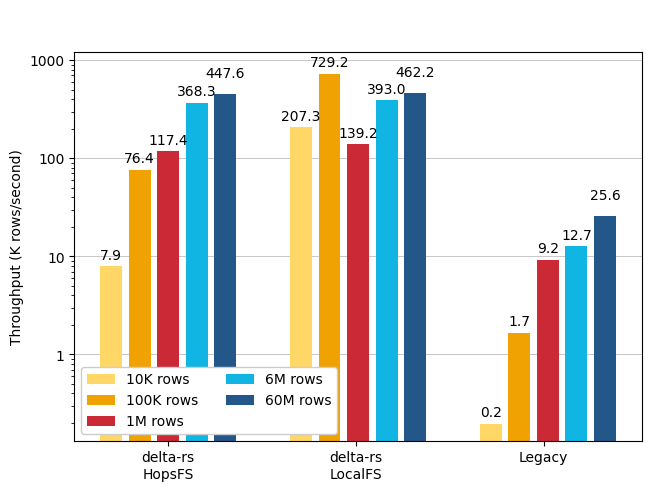
\includegraphics[width=\textwidth]{figures/99-appendix/results-diagrams/write/write_throughput_2_core.png}
        \caption[Histogram of the write experiment - Throughput - 2 CPU cores]{Histogram in log-scale of the write experiment results expressed as throughput. The experiment was performed with two \glstext{CPU} cores.}
        \label{fig:appx_res_write_throughput_2_cores}
    \end{minipage}
\end{figure}

\begin{figure}
    \centering
    \begin{minipage}[b]{\textwidth}
        \centering
        \captionof{table}[Write experiment - Throughput - 4 CPU cores]{Write experiment results expressed as throughput. The experiment was performed with four \glstext{CPU} cores.}
        \label{tbl:appx_res_write_throughput_4_cores}
        \begin{tabular}{c r S[table-format=5.5] S[table-format=5.5] S[table-format=5.5]} 
            \toprule
            \multirow{2}{*}{{Pipeline\Tstrut\Bstrut}} & \multirow{2}{*}{{\thead{Number\\ of rows}}} & {\multirow{2}{*}{{\thead{Throughput \\ (k rows/second)}}}} & \multicolumn{2}{c}{{\thead{Throughput (k rows/second) \\95\% Confidence Interval}}}\\
                                                      &                                             &                                                          & {low} & {high}\\
            \midrule
            \multirow{5}{4em}{delta-rs\\ HopsFS} & 10K  &    8.22083 &    8.11482 &   8.11482\\ 
                                                 & 100K &   74.83742 &   74.10566 &  75.58871\\ 
                                                 & 1M   &  118.86008 &  116.51310 & 121.24582\\
                                                 & 6M   &  369.82202 &  361.53577 & 377.84652\\
                                                 & 60M  &  483.47160 &  473.12899 & 493.51343\\
            \midrule
            \multirow{5}{4em}{delta-rs\\ LocalFS} & 10K  &  218.71364 &  208.02604 &  230.31412\\ 
                                                  & 100K &  758.92422 &  740.79474 &  776.39115\\ 
                                                  & 1M   &  139.16432 &  135.80613 &  142.71864\\
                                                  & 6M   &  412.20728 &  401.55459 &  423.22678\\
                                                  & 60M  &  494.33070 &  485.04875 &  503.47156\\
            \midrule
            \multirow{5}{4em}{Legacy} & 10K  &     0.19499 &    0.19266 &    0.19753\\ 
                                      & 100K &     1.67992 &    1.66242 &    1.69763\\ 
                                      & 1M   &     9.18976 &    9.14558 &    9.23768\\
                                      & 6M   &    12.44855 &   12.42416 &   12.47286\\
                                      & 60M  &    25.57493 &   25.47555 &   25.67400\\
            \bottomrule
        \end{tabular}
    \end{minipage}
    \begin{minipage}[b]{\textwidth}
        \centering
        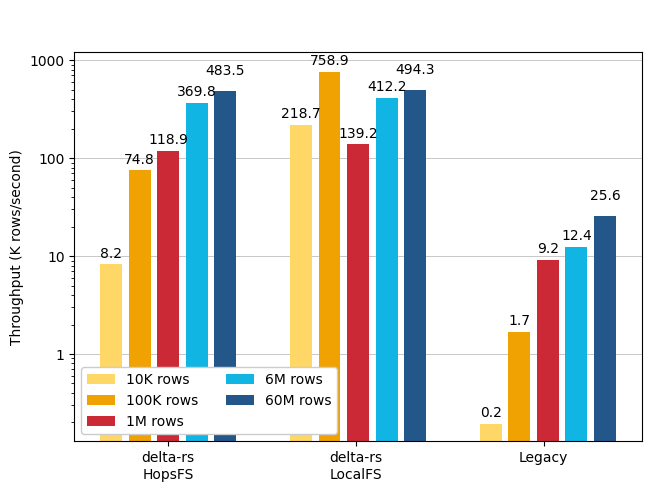
\includegraphics[width=\textwidth]{figures/99-appendix/results-diagrams/write/write_throughput_4_core.png}
        \caption[Histogram of the write experiment - Throughput - 4 CPU cores]{Histogram in log-scale of the write experiment results expressed as throughput. The experiment was performed with four \glstext{CPU} cores.}
        \label{fig:appx_res_write_throughput_4_cores}
    \end{minipage}
\end{figure}

\begin{figure}
    \centering
    \begin{minipage}[b]{\textwidth}
        \centering
        \captionof{table}[Write experiment - Throughput - 8 CPU cores]{Write experiment results expressed as throughput. The experiment was performed with eight \glstext{CPU} cores.}
        \label{tbl:appx_res_write_throughput_8_cores}
        \begin{tabular}{c r S[table-format=5.5] S[table-format=5.5] S[table-format=5.5]} 
            \toprule
            \multirow{2}{*}{{Pipeline\Tstrut\Bstrut}} & \multirow{2}{*}{{\thead{Number\\ of rows}}} & {\multirow{2}{*}{{\thead{Throughput \\ (k rows/second)}}}} & \multicolumn{2}{c}{{\thead{Throughput (k rows/second) \\95\% Confidence Interval}}}\\
                                                      &                                             &                                                          & {low} & {high}\\
            \midrule
            \multirow{5}{4em}{delta-rs\\ HopsFS} & 10K  &    7.31228 &    6.36032 &    8.00422\\ 
                                                 & 100K &   77.37337 &   76.27782 &   79.02104\\ 
                                                 & 1M   &  120.46439 &  118.05814 &  122.71160\\
                                                 & 6M   &  381.23126 &  371.26772 &  392.41978\\
                                                 & 60M  &  492.00431 &  483.16579 &  501.69837\\
            \midrule
            \multirow{5}{4em}{delta-rs\\ LocalFS} & 10K  &  227.12095 &  215.48714 &  239.54128\\ 
                                                  & 100K &  732.70141 &  711.16038 &  752.93200\\ 
                                                  & 1M   &  138.33701 &  135.15466 &  141.34041\\
                                                  & 6M   &  420.12165 &  409.24176 &  431.49669\\
                                                  & 60M  &  500.08688 &  490.96288 &  509.49286\\
            \midrule
            \multirow{5}{4em}{Legacy} & 10K  &     0.19520 &    0.19280 &    0.19764\\ 
                                      & 100K &     1.65899 &    1.64551 &    1.67422\\ 
                                      & 1M   &     9.14228 &    9.10061 &    9.18540\\
                                      & 6M   &    12.60653 &   12.57722 &   12.63583\\
                                      & 60M  &    25.80668 &   25.73949 &   25.87275\\
            \bottomrule
        \end{tabular}
    \end{minipage}
    \begin{minipage}[b]{\textwidth}
        \centering
        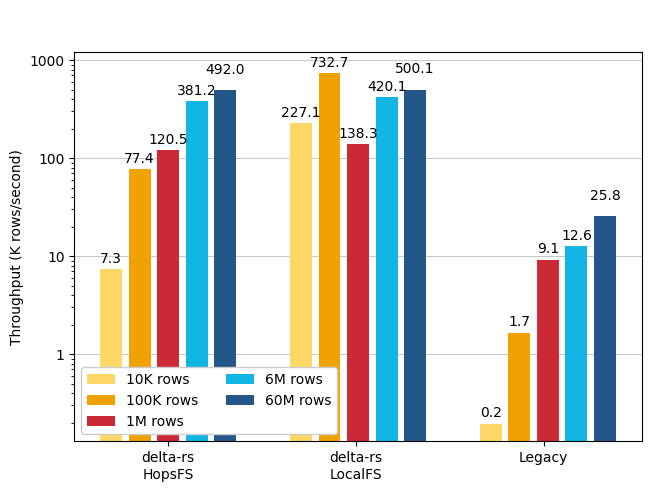
\includegraphics[width=\textwidth]{figures/99-appendix/results-diagrams/write/write_throughput_8_core.png}
        \caption[Histogram of the write experiment - Throughput - 8 CPU cores]{Histogram in log-scale of the write experiment results expressed as throughput. The experiment was performed with eight \glstext{CPU} cores.}
        \label{fig:appx_res_write_throughput_8_cores}
    \end{minipage}
\end{figure}

\chapter{Read experiments results}
    \label{appx:res_read}
    % Brief expl
This appendix reports all graphs and tables related to the read experiments conducted. Results are reported first expressed as latency (measured during the experiments) and then as throughput (computed from the latency and table size).


%%%%%%%%%%%%%%%%%%%%%%%%%%%%%%%%%%%%%%%%%%%%%%%%%%%%%%%%%%%%%%%%%
%%%%%%%%%%%%              LATENCY             %%%%%%%%%%%%%%%%%%%
%%%%%%%%%%%%%%%%%%%%%%%%%%%%%%%%%%%%%%%%%%%%%%%%%%%%%%%%%%%%%%%%%
\begin{figure}
    \centering
    \begin{minipage}[b]{\textwidth}
        \centering
        \captionof{table}[Read experiment - Latency - 1 CPU core]{Read experiment results expressed as latency. The experiment was performed with one \glstext{CPU} core.}
        \label{tbl:appx_res_read_time_1_core}
        \begin{tabular}{c r S[table-format=5.5] S[table-format=5.5] S[table-format=5.5]} 
            \toprule
            \multirow{2}{*}{{Pipeline\Tstrut\Bstrut}} & \multirow{2}{*}{{\thead{Number\\ of rows}}} & {\multirow{2}{*}{{\thead{Latency \\ (seconds)}}}} & \multicolumn{2}{c}{{\thead{Latency (seconds) \\95\% Confidence Interval}}}\\
                                                      &                                             &                                                   & {low} & {high}\\
            \midrule
            \multirow{5}{4em}{delta-rs\\ HopsFS} & 10K  &    0.05342 &    0.03916 &    0.08112\\ 
                                                 & 100K &    0.05757 &    0.05518 &    0.06046\\ 
                                                 & 1M   &    0.53855 &    0.52558 &    0.55229\\
                                                 & 6M   &    1.94899 &    1.93007 &    1.96860\\
                                                 & 60M  &   22.98065 &   22.84067 &   23.14206\\
            \midrule
            \multirow{5}{4em}{delta-rs\\ LocalFS} & 10K  &    0.00419 &    0.00268 &    0.00644\\ 
                                                  & 100K &    0.02696 &    0.01966 &    0.03433\\ 
                                                  & 1M   &    0.42009 &    0.40613 &    0.43563\\
                                                  & 6M   &    1.68223 &    1.65981 &    1.70440\\
                                                  & 60M  &   19.56547 &   19.34690 &   19.77724\\
            \midrule
            \multirow{5}{4em}{Legacy} & 10K  &     0.63159 &    0.62414 &    0.64157\\ 
                                      & 100K &     2.65010 &    2.64272 &    2.65876\\ 
                                      & 1M   &     8.59636 &    8.34094 &    8.90047\\
                                      & 6M   &    33.52964 &   33.23886 &   33.86591\\
                                      & 60M  &    33.69772 &   33.36262 &   34.08665\\
            \bottomrule
        \end{tabular}
    \end{minipage}
    \begin{minipage}[b]{\textwidth}
        \centering
        \includegraphics[width=\textwidth]{figures/99-appendix/results-diagrams/read/read_time_1_core.png}
        \caption[Histogram of the read experiment - Latency - 1 CPU core]{Histogram in log-scale of the read experiment results expressed as latency. The experiment was performed with one \glstext{CPU} core.}
        \label{fig:appx_res_read_time_1_core}
    \end{minipage}
\end{figure}

\begin{figure}
    \centering
    \begin{minipage}[b]{\textwidth}
        \centering
        \captionof{table}[Read experiment - Latency - 2 CPU cores]{Read experiment results expressed as latency. The experiment was performed with two \glstext{CPU} cores.}
        \label{tbl:appx_res_read_time_2_cores}
        \begin{tabular}{c r S[table-format=5.5] S[table-format=5.5] S[table-format=5.5]} 
            \toprule
            \multirow{2}{*}{{Pipeline\Tstrut\Bstrut}} & \multirow{2}{*}{{\thead{Number\\ of rows}}} & {\multirow{2}{*}{{\thead{Latency \\ (seconds)}}}} & \multicolumn{2}{c}{{\thead{Latency (seconds) \\95\% Confidence Interval}}}\\
                                                      &                                             &                                                   & {low} & {high}\\
            \midrule
            \multirow{5}{4em}{delta-rs\\ HopsFS} & 10K  &    0.04132 &    0.03933 &    0.04378\\ 
                                                 & 100K &    0.05690 &    0.05123 &    0.06693\\ 
                                                 & 1M   &    0.23413 &    0.22528 &    0.24426\\
                                                 & 6M   &    0.90832 &    0.89967 &    0.91744\\
                                                 & 60M  &   11.41325 &   11.27661 &   11.58899\\
            \midrule
            \multirow{5}{4em}{delta-rs\\ LocalFS} & 10K  &    0.00287 &    0.00278 &    0.00299\\ 
                                                  & 100K &    0.01306 &    0.01041 &    0.01610\\ 
                                                  & 1M   &    0.19977 &    0.18858 &    0.21056\\
                                                  & 6M   &    0.74764 &    0.73503 &    0.76013\\
                                                  & 60M  &    9.44693 &    9.37207 &    9.51753\\
            \midrule
            \multirow{5}{4em}{Legacy} & 10K  &     0.62492 &    0.62210 &    0.62822\\ 
                                      & 100K &     2.66339 &    2.65616 &    2.67166\\ 
                                      & 1M   &     8.61667 &    8.30989 &    8.94938\\
                                      & 6M   &    33.37519 &   33.09688 &   33.67065\\
                                      & 60M  &    33.64281 &   33.30150 &   34.06307\\
            \bottomrule
        \end{tabular}
    \end{minipage}
    \begin{minipage}[b]{\textwidth}
        \centering
        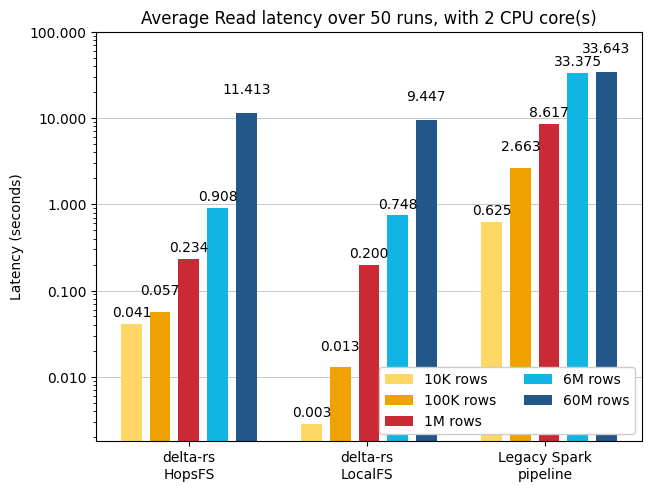
\includegraphics[width=\textwidth]{figures/99-appendix/results-diagrams/read/read_time_2_core.png}
        \caption[Histogram of the read experiment - Latency - 2 CPU cores]{Histogram in log-scale of the read experiment results expressed as latency. The experiment was performed with two \glstext{CPU} cores.}
        \label{fig:appx_res_read_time_2_cores}
    \end{minipage}
\end{figure}

\begin{figure}
    \centering
    \begin{minipage}[b]{\textwidth}
        \centering
        \captionof{table}[Read experiment - Latency - 4 CPU cores]{Read experiment results expressed as latency. The experiment was performed with four \glstext{CPU} cores.}
        \label{tbl:appx_res_read_time_4_cores}
        \begin{tabular}{c r S[table-format=5.5] S[table-format=5.5] S[table-format=5.5]} 
            \toprule
            \multirow{2}{*}{{Pipeline\Tstrut\Bstrut}} & \multirow{2}{*}{{\thead{Number\\ of rows}}} & {\multirow{2}{*}{{\thead{Latency \\ (seconds)}}}} & \multicolumn{2}{c}{{\thead{Latency (seconds) \\95\% Confidence Interval}}}\\
                                                      &                                             &                                                   & {low} & {high}\\
            \midrule
            \multirow{5}{4em}{delta-rs\\ HopsFS} & 10K  &    0.04336 &    0.03922 &   0.05092\\ 
                                                 & 100K &    0.05540 &    0.05378 &   0.05789\\ 
                                                 & 1M   &    0.18847 &    0.15157 &   0.25189\\
                                                 & 6M   &    0.53124 &    0.50778 &   0.57105\\
                                                 & 60M  &    5.58011 &    5.54397 &   5.61936\\
            \midrule
            \multirow{5}{4em}{delta-rs\\ LocalFS} & 10K  &    0.00268 &   0.00259 &   0.00279\\ 
                                                  & 100K &    0.00923 &   0.00852 &   0.01020\\ 
                                                  & 1M   &    0.08971 &   0.08388 &   0.09503\\
                                                  & 6M   &    0.37021 &   0.36018 &   0.38032\\
                                                  & 60M  &    4.81023 &   4.79338 &   4.82789\\
            \midrule
            \multirow{5}{4em}{Legacy} & 10K  &     0.63583 &    0.62352 &    0.65908\\ 
                                      & 100K &     2.63985 &    2.63349 &    2.64623\\ 
                                      & 1M   &     8.75238 &    8.50725 &    9.01383\\
                                      & 6M   &    33.45286 &   33.19461 &   33.75646\\
                                      & 60M  &    33.65245 &   33.27016 &   34.03900\\
            \bottomrule
        \end{tabular}
    \end{minipage}
    \begin{minipage}[b]{\textwidth}
        \centering
        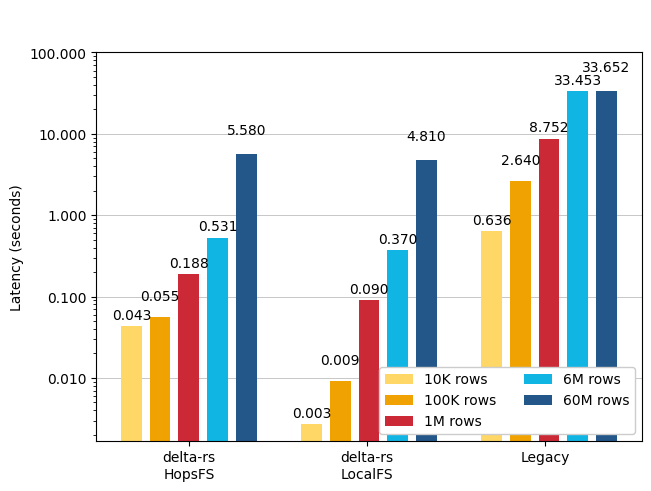
\includegraphics[width=\textwidth]{figures/99-appendix/results-diagrams/read/read_time_4_core.png}
        \caption[Histogram of the read experiment - Latency - 4 CPU cores]{Histogram in log-scale of the read experiment results expressed as latency. The experiment was performed with four \glstext{CPU} cores.}
        \label{fig:appx_res_read_time_4_cores}
    \end{minipage}
\end{figure}

\begin{figure}
    \centering
    \begin{minipage}[b]{\textwidth}
        \centering
        \captionof{table}[Read experiment - Latency - 8 CPU cores]{Read experiment results expressed as latency. The experiment was performed with eight \glstext{CPU} cores.}
        \label{tbl:appx_res_read_time_8_cores}
        \begin{tabular}{c r S[table-format=5.5] S[table-format=5.5] S[table-format=5.5]} 
            \toprule
            \multirow{2}{*}{{Pipeline\Tstrut\Bstrut}} & \multirow{2}{*}{{\thead{Number\\ of rows}}} & {\multirow{2}{*}{{\thead{Latency \\ (seconds)}}}} & \multicolumn{2}{c}{{\thead{Latency (seconds) \\95\% Confidence Interval}}}\\
                                                      &                                             &                                                   & {low} & {high}\\
            \midrule
            \multirow{5}{4em}{delta-rs\\ HopsFS} & 10K  &    0.04330 &    0.03885 &    0.05119\\ 
                                                 & 100K &    0.05458 &    0.05286 &    0.05663\\ 
                                                 & 1M   &    0.17390 &    0.16992 &    0.17808\\
                                                 & 6M   &    0.49729 &    0.48655 &    0.51019\\
                                                 & 60M  &    2.94236 &    2.85554 &    3.06360\\
            \midrule
            \multirow{5}{4em}{delta-rs\\ LocalFS} & 10K  &    0.00294 &    0.00284 &    0.00307\\ 
                                                  & 100K &    0.00948 &    0.00872 &    0.01056\\ 
                                                  & 1M   &    0.04308 &    0.03934 &    0.04830\\
                                                  & 6M   &    0.17548 &    0.17009 &    0.18080\\
                                                  & 60M  &    2.28550 &    2.27501 &    2.29607\\
            \midrule
            \multirow{5}{4em}{Legacy} & 10K  &     0.62739 &    0.62245 &    0.63259\\ 
                                      & 100K &     2.66217 &    2.65309 &    2.67218\\ 
                                      & 1M   &     8.34757 &    8.13471 &    8.60942\\
                                      & 6M   &    33.42815 &   33.15376 &   33.74947\\
                                      & 60M  &    33.14341 &   32.88303 &   33.41299\\
            \bottomrule
        \end{tabular}
    \end{minipage}
    \begin{minipage}[b]{\textwidth}
        \centering
        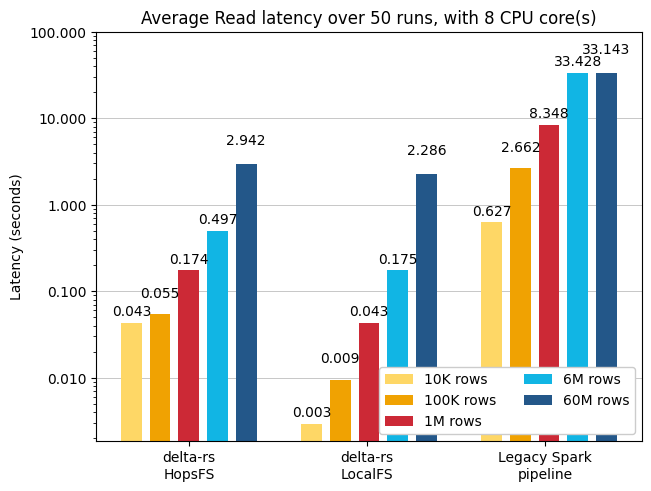
\includegraphics[width=\textwidth]{figures/99-appendix/results-diagrams/read/read_time_8_core.png}
        \caption[Histogram of the read experiment - Latency - 8 CPU cores]{Histogram in log-scale of the read experiment results expressed as latency. The experiment was performed with eight \glstext{CPU} cores.}
        \label{fig:appx_res_read_time_8_cores}
    \end{minipage}
\end{figure}

%%%%%%%%%%%%%%%%%%%%%%%%%%%%%%%%%%%%%%%%%%%%%%%%%%%%%%%%%%%%%%%%%
%%%%%%%%%%%%             THROUGHPUT           %%%%%%%%%%%%%%%%%%%
%%%%%%%%%%%%%%%%%%%%%%%%%%%%%%%%%%%%%%%%%%%%%%%%%%%%%%%%%%%%%%%%%

\begin{figure}
    \centering
    \begin{minipage}[b]{\textwidth}
        \centering
        \captionof{table}[Read experiment - Throughput - 1 CPU core]{Read experiment results expressed as throughput. The experiment was performed with one \glstext{CPU} core.}
        \label{tbl:appx_res_read_throughput_1_core}
        \begin{tabular}{c r S[table-format=5.5] S[table-format=5.5] S[table-format=5.5]} 
            \toprule
            \multirow{2}{*}{{Pipeline\Tstrut\Bstrut}} & \multirow{2}{*}{{\thead{Number\\ of rows}}} & {\multirow{2}{*}{{\thead{Throughput \\ (k rows/second)}}}} & \multicolumn{2}{c}{{\thead{Throughput (k rows/second) \\95\% Confidence Interval}}}\\
                                                      &                                             &                                                          & {low} & {high}\\
            \midrule
            \multirow{5}{4em}{delta-rs\\ HopsFS} & 10K  &  187.16853 &  123.26555 &  255.36173\\ 
                                                 & 100K & 1736.90799 & 1653.91940 & 1811.92857\\ 
                                                 & 1M   & 1856.83167 & 1810.61318 & 1902.65361\\
                                                 & 6M   & 3078.51299 & 3047.83914 & 3108.69431\\
                                                 & 60M  & 2610.89146 & 2592.68185 & 2626.89240\\
            \midrule
            \multirow{5}{4em}{delta-rs\\ LocalFS} & 10K  & 2384.58699 & 1552.08552 & 3721.36068\\ 
                                                  & 100K & 3708.25787 & 2912.43600 & 5084.75715\\ 
                                                  & 1M   & 2380.40381 & 2295.50154 & 2462.25814\\
                                                  & 6M   & 3566.67454 & 3520.29796 & 3614.87006\\
                                                  & 60M  & 3066.62644 & 3033.78996 & 3101.27165\\
            \midrule
            \multirow{5}{4em}{Legacy} & 10K  &    15.83285 &   15.58654 &   16.02196\\ 
                                      & 100K &    37.73432 &   37.61140 &   37.83975\\ 
                                      & 1M   &   116.32820 &  112.35350 &  119.89044\\
                                      & 6M   &   178.94612 &  177.16928 &  180.51159\\
                                      & 60M  &  1780.53563 & 1760.21974 & 1798.41962\\
            \bottomrule
        \end{tabular}
    \end{minipage}
    \begin{minipage}[b]{\textwidth}
        \centering
        \includegraphics[width=\textwidth]{figures/99-appendix/results-diagrams/read/read_throughput_1_core.png}
        \caption[Histogram of the read experiment - Throughput - 1 CPU core]{Histogram in log-scale of the read experiment results expressed as throughput. The experiment was performed with one \glstext{CPU} core.}
        \label{fig:appx_res_read_throughput_1_core}
    \end{minipage}
\end{figure}

\begin{figure}
    \centering
    \begin{minipage}[b]{\textwidth}
        \centering
        \captionof{table}[Read experiment - Throughput - 2 CPU cores]{Read experiment results expressed as throughput. The experiment was performed with two \glstext{CPU} cores.}
        \label{tbl:appx_res_read_throughput_2_cores}
        \begin{tabular}{c r S[table-format=5.5] S[table-format=5.5] S[table-format=5.5]} 
            \toprule
            \multirow{2}{*}{{Pipeline\Tstrut\Bstrut}} & \multirow{2}{*}{{\thead{Number\\ of rows}}} & {\multirow{2}{*}{{\thead{Throughput \\ (k rows/second)}}}} & \multicolumn{2}{c}{{\thead{Throughput (k rows/second) \\95\% Confidence Interval}}}\\
                                                      &                                             &                                                          & {low} & {high}\\
            \midrule
            \multirow{5}{4em}{delta-rs\\ HopsFS} & 10K  &  241.97833 &  228.37018 &  254.22419\\ 
                                                 & 100K & 1757.17930 & 1494.01876 & 1951.81229\\ 
                                                 & 1M   & 4271.12139 & 4093.98917 & 4438.84612\\
                                                 & 6M   & 6605.54323 & 6539.93631 & 6669.08756\\
                                                 & 60M  & 5257.04658 & 5177.32395 & 5320.74334\\
            \midrule
            \multirow{5}{4em}{delta-rs\\ LocalFS} & 10K  & 3479.95285 & 3339.11982 & 3592.42255\\ 
                                                  & 100K & 7652.74709 & 6210.29638 & 9604.33293\\ 
                                                  & 1M   & 5005.61642 & 4749.17943 & 5302.53656\\
                                                  & 6M   & 8025.19634 & 7893.33251 & 8162.84493\\
                                                  & 60M  & 6351.26715 & 6304.15538 & 6401.99467\\
            \midrule
            \multirow{5}{4em}{Legacy} & 10K  &   16.00183 &   15.91773 &   16.07453\\ 
                                      & 100K &   37.54607 &   37.42979 &   37.64822\\ 
                                      & 1M   &  116.05404 &  111.73951 &  120.33848\\
                                      & 6M   &  179.77424 &  178.19671 &  181.28593\\
                                      & 60M  & 1783.44198 & 1761.43830 & 1801.72013\\
            \bottomrule
        \end{tabular}
    \end{minipage}
    \begin{minipage}[b]{\textwidth}
        \centering
        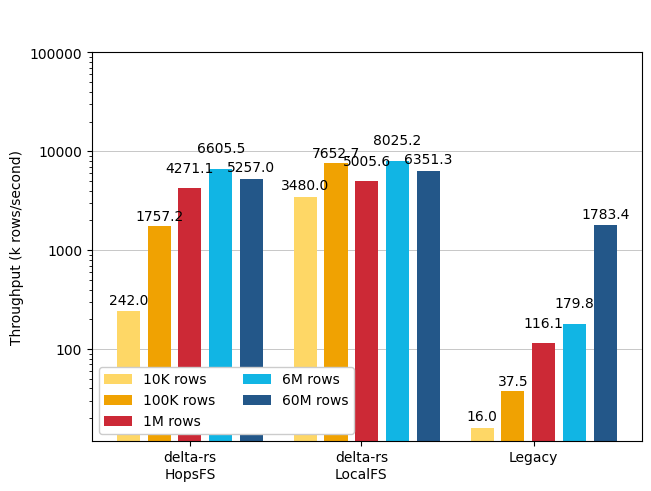
\includegraphics[width=\textwidth]{figures/99-appendix/results-diagrams/read/read_throughput_2_core.png}
        \caption[Histogram of the read experiment - Throughput - 2 CPU cores]{Histogram in log-scale of the read experiment results expressed as throughput. The experiment was performed with two \glstext{CPU} cores.}
        \label{fig:appx_res_read_throughput_2_cores}
    \end{minipage}
\end{figure}

\begin{figure}
    \centering
    \begin{minipage}[b]{\textwidth}
        \centering
        \captionof{table}[Read experiment - Throughput - 4 CPU cores]{Read experiment results expressed as throughput. The experiment was performed with four \glstext{CPU} cores.}
        \label{tbl:appx_res_read_throughput_4_cores}
        \begin{tabular}{c r S[table-format=5.5] S[table-format=5.5] S[table-format=5.5]} 
            \toprule
            \multirow{2}{*}{{Pipeline\Tstrut\Bstrut}} & \multirow{2}{*}{{\thead{Number\\ of rows}}} & {\multirow{2}{*}{{\thead{Throughput \\ (k rows/second)}}}} & \multicolumn{2}{c}{{\thead{Throughput (k rows/second) \\95\% Confidence Interval}}}\\
                                                      &                                             &                                                          & {low} & {high}\\
            \midrule
            \multirow{5}{4em}{delta-rs\\ HopsFS} & 10K  &   230.61925 &   196.37366 &   254.93232\\ 
                                                 & 100K &  1804.73106 &  1727.27256 &  1859.40719\\ 
                                                 & 1M   &  5305.74239 &  3969.95699 &  6597.37404\\
                                                 & 6M   & 11294.12619 & 10506.91939 & 11816.03313\\
                                                 & 60M  & 10752.47511 & 10677.35647 & 10822.55620\\
            \midrule
            \multirow{5}{4em}{delta-rs\\ LocalFS} & 10K  &  3720.94104 &  3572.45085 &  3854.74973\\ 
                                                  & 100K & 10830.88457 &  9802.96062 & 11735.92863\\ 
                                                  & 1M   & 11146.06743 & 10522.54071 & 11921.62257\\
                                                  & 6M   & 16206.97330 & 15775.94387 & 16657.93725\\
                                                  & 60M  & 12473.40492 & 12427.78728 & 12517.25967\\
            \midrule
            \multirow{5}{4em}{Legacy} & 10K  &    15.72724 &   15.17259 &   16.03790\\ 
                                      & 100K &    37.88093 &   37.78959 &   37.97237\\ 
                                      & 1M   &   114.25460 &  110.94061 &  117.54671\\
                                      & 6M   &   179.35680 &  177.74372 &  180.75222\\
                                      & 60M  &  1782.93073 & 1762.68396 & 1803.41764\\
            \bottomrule
        \end{tabular}
    \end{minipage}
    \begin{minipage}[b]{\textwidth}
        \centering
        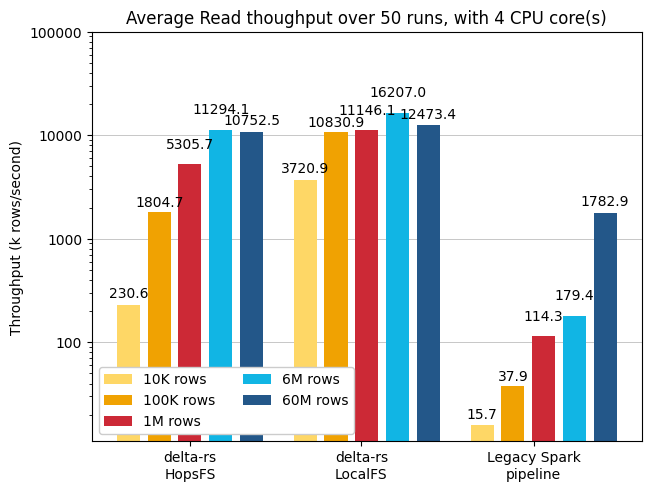
\includegraphics[width=\textwidth]{figures/99-appendix/results-diagrams/read/read_throughput_4_core.png}
        \caption[Histogram of the read experiment - Throughput - 4 CPU cores]{Histogram in log-scale of the read experiment results expressed as throughput. The experiment was performed with four \glstext{CPU} cores.}
        \label{fig:appx_res_read_throughput_4_cores}
    \end{minipage}
\end{figure}

\begin{figure}
    \centering
    \begin{minipage}[b]{\textwidth}
        \centering
        \captionof{table}[Read experiment - Throughput - 8 CPU cores]{Read experiment results expressed as throughput. The experiment was performed with eight \glstext{CPU} cores.}
        \label{tbl:appx_res_read_throughput_8_cores}
        \begin{tabular}{c r S[table-format=5.5] S[table-format=5.5] S[table-format=5.5]} 
            \toprule
            \multirow{2}{*}{{Pipeline\Tstrut\Bstrut}} & \multirow{2}{*}{{\thead{Number\\ of rows}}} & {\multirow{2}{*}{{\thead{Throughput \\ (k rows/second)}}}} & \multicolumn{2}{c}{{\thead{Throughput (k rows/second) \\95\% Confidence Interval}}}\\
                                                      &                                             &                                                          & {low} & {high}\\
            \midrule
            \multirow{5}{4em}{delta-rs\\ HopsFS} & 10K  &   230.92518 &   195.34544 &   257.36067\\ 
                                                 & 100K &  1832.05683 &  1765.75684 &  1891.54456\\ 
                                                 & 1M   &  5750.34366 &  5615.17071 &  5885.01795\\
                                                 & 6M   & 12065.18202 & 11760.17893 & 12331.70977\\
                                                 & 60M  & 20391.77956 & 19584.75363 & 21011.72136\\
            \midrule
            \multirow{5}{4em}{delta-rs\\ LocalFS} & 10K  &  3390.32242 &  3256.07486 &  3510.69231\\ 
                                                  & 100K & 10545.41087 &  9465.27536 & 11463.06073\\ 
                                                  & 1M   & 23212.46679 & 20701.23033 & 25414.13122\\
                                                  & 6M   & 34191.39637 & 33185.18129 & 35275.25456\\
                                                  & 60M  & 26252.42019 & 26131.51836 & 26373.48880\\
            \midrule
            \multirow{5}{4em}{Legacy} & 10K  &    15.93901 &   15.80791 &   16.06539\\ 
                                      & 100K &    37.56330 &   37.42250 &   37.69186\\ 
                                      & 1M   &   119.79520 &  116.15177 &  122.92995\\
                                      & 6M   &   179.48942 &  177.78054 &  180.97490\\
                                      & 60M  &  1810.31436 & 1795.70867 & 1824.64883\\
            \bottomrule
        \end{tabular}
    \end{minipage}
    \begin{minipage}[b]{\textwidth}
        \centering
        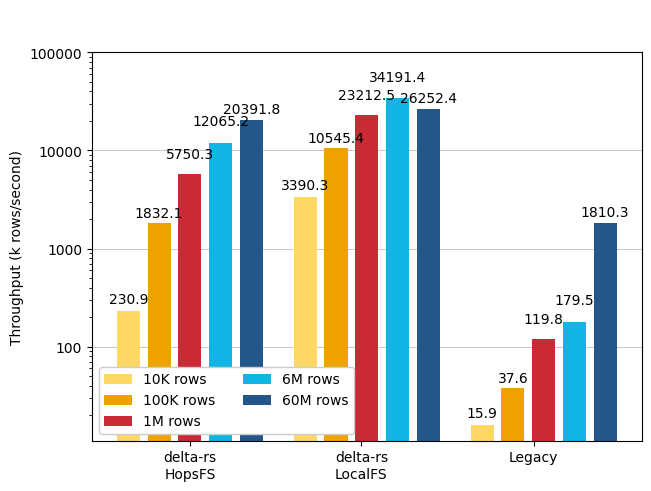
\includegraphics[width=\textwidth]{figures/99-appendix/results-diagrams/read/read_throughput_8_core.png}
        \caption[Histogram of the read experiment - Throughput - 8 CPU cores]{Histogram in log-scale of the read experiment results expressed as throughput. The experiment was performed with eight \glstext{CPU} cores.}
        \label{fig:appx_res_read_throughput_8_cores}
    \end{minipage}
\end{figure}

\chapter{Legacy pipeline write latency breakdown results}
    \label{appx:res_hudi}
    % Brief expl
This appendix reports all graphs and tables related to all write latency breakdown of the upload and materialization steps in the legacy pipeline.

\begin{figure}
    \centering
    \begin{minipage}[b]{\textwidth}
        \centering
        \captionof{table}[Write on legacy pipeline - Time breakdown - 1 core]{Contributions to the write latency of the upload and materialization steps in the legacy pipeline. The experiment was performed with one \glstext{CPU} core.}
        \label{tbl:appx_hudi_virtualiz_breakdown_1_core}
        \begin{tabular}{l r S[table-format=5.4] S[table-format=5.4] S[table-format=5.4] S[table-format=5.4]} 
            \toprule
            {\multirow{2}{*}{Step\Tstrut\Bstrut}} & \multirow{2}{*}{{\thead{Number\\ of rows}}} & {\multirow{2}{*}{{\thead{Latency \\ (seconds)}}}} & \multicolumn{2}{c}{{\thead{Latency (seconds) \\95\% Confidence Interval}}}\\
                                    &                                             &                                                   & {low} & {high}                                                            \\
            \midrule
            upload                  & \multirow{2}{*}{10K}                        &    2.4865                                         &    2.3896 &    2.6261                                                      \\ 
            materialize           &                                             &   47.7262                                         &   47.0445 &   48.4031                                                      \\
            \midrule
            upload                  & \multirow{2}{*}{100K}                       &    3.6684                                         &    3.6310 &    3.7098                                                      \\                                                                 
            materialize            &                                             &   55.9005                                         &   55.2494 &   56.5541                                                      \\
            \midrule
            upload                  & \multirow{2}{*}{1M}                         &   22.5934                                         &   22.4496 &   22.7349                                                      \\                                                                 
            materialize             &                                             &   89.5754                                         &   88.8286 &   90.3049                                                      \\
            \midrule
            upload                 & \multirow{2}{*}{6M}                         &  244.6123                                         &  244.0368 &  245.1905                                                      \\                                                                 
            materialize             &                                             &  267.2490                                         &  266.4287 &  268.1549                                                      \\
            \midrule
            upload                  & \multirow{2}{*}{60M}                         & 2437.7840                                         & 2422.8704 & 2453.6746                                                      \\                                                                 
            materialize             &                                             &  278.0504                                         &  276.2340 &  280.0921                                                      \\
            \bottomrule
        \end{tabular}
    \end{minipage}
    \begin{minipage}[b]{\textwidth}
        \centering
        \includegraphics[width=\textwidth]{figures/99-appendix/results-diagrams/write/hudi_upload_materialize/hudi_virtualiz_1_core.png}
        \caption[Histogram of the write on legacy pipeline - Time breakdown - 1 CPU core]{Histogram in log-scale displaying the contributions to the write latency of the upload and materialization steps in the legacy pipeline. The experiment was performed with one \glstext{CPU} core.}
        \label{fig:appx_hudi_virtualiz_breakdown_1_core}
    \end{minipage}
\end{figure}

\begin{figure}
    \centering
    \begin{minipage}[b]{\textwidth}
        \centering
        \captionof{table}[Write on legacy pipeline - Time breakdown - 2 cores]{Contributions to the write latency of the upload and materialization steps in the legacy pipeline. The experiment was performed with two \glstext{CPU} cores.}
        \label{tbl:appx_hudi_virtualiz_breakdown_2_cores}
        \begin{tabular}{l r S[table-format=5.4] S[table-format=5.4] S[table-format=5.4] S[table-format=5.4]} 
            \toprule
            {\multirow{2}{*}{Step\Tstrut\Bstrut}} & \multirow{2}{*}{{\thead{Number\\ of rows}}} & {\multirow{2}{*}{{\thead{Latency \\ (seconds)}}}} & \multicolumn{2}{c}{{\thead{Latency (seconds) \\95\% Confidence Interval}}}\\
                                    &                                             &                                                   & {low} & {high}                                                            \\
            \midrule
            upload                  & \multirow{2}{*}{10K}                        &    2.3873                                         &    2.3276 &    2.4466                                                      \\ 
            materialize             &                                             &   48.3305                                         &   47.7020 &   48.9923                                                      \\
            \midrule
            upload                  & \multirow{2}{*}{100K}                       &    3.4348                                         &    3.4008 &    3.4671                                                      \\                                                                 
            materialize             &                                             &   56.3367                                         &   55.5626 &   57.1129                                                      \\
            \midrule
            upload                  & \multirow{2}{*}{1M}                         &   18.6349                                         &   18.5673 &   18.7104                                                      \\                                                                 
            materialize             &                                             &   89.9267                                         &   89.4012 &   90.4514                                                      \\
            \midrule
            upload                  & \multirow{2}{*}{6M}                         &  205.8854                                         &  205.2177 &  206.4984                                                      \\                                                                 
            materialize             &                                             &  267.5079                                         &  266.6853 &  268.3512                                                      \\
            \midrule
            upload                  & \multirow{2}{*}{60M}                         & 2064.1357                                         & 2057.6396 & 2070.4450                                                      \\                                                                 
            materialize             &                                             &  276.9608                                         &  275.7156 &  278.2849                                                      \\
            \bottomrule
        \end{tabular}
    \end{minipage}
    \begin{minipage}[b]{\textwidth}
        \centering
        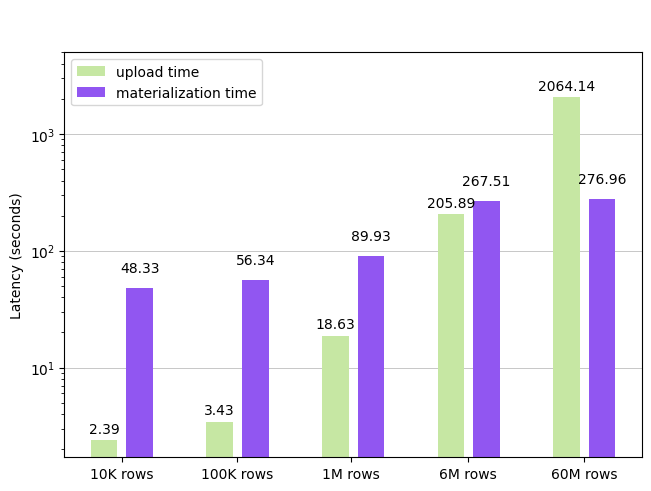
\includegraphics[width=\textwidth]{figures/99-appendix/results-diagrams/write/hudi_upload_materialize/hudi_virtualiz_2_core.png}
        \caption[Histogram of the write on legacy pipeline - Time breakdown - 2 CPU cores]{Histogram in log-scale displaying the contributions to the write latency of the upload and materialization steps in the legacy pipeline. The experiment was performed with two \glstext{CPU} cores.}
        \label{fig:appx_hudi_virtualiz_breakdown_2_core}
    \end{minipage}
\end{figure}

\begin{figure}
    \centering
    \begin{minipage}[b]{\textwidth}
        \centering
        \captionof{table}[Write on legacy pipeline - Time breakdown - 4 cores]{Contributions to the write latency of the upload and materialization steps in the legacy pipeline. The experiment was performed with four \glstext{CPU} cores.}
        \label{tbl:appx_hudi_virtualiz_breakdown_4_cores}
        \begin{tabular}{l r S[table-format=5.4] S[table-format=5.4] S[table-format=5.4] S[table-format=5.4]} 
            \toprule
            {\multirow{2}{*}{Step\Tstrut\Bstrut}} & \multirow{2}{*}{{\thead{Number\\ of rows}}} & {\multirow{2}{*}{{\thead{Latency \\ (seconds)}}}} & \multicolumn{2}{c}{{\thead{Latency (seconds) \\95\% Confidence Interval}}}\\
                                    &                                             &                                                   & {low} & {high}                                                            \\
            \midrule
            upload                  & \multirow{2}{*}{10K}                        &    2.3846                                         &    2.3299 &    2.4335                                                      \\ 
            materialize             &                                             &   48.9061                                         &   48.2436 &   49.5470                                                      \\
            \midrule
            upload                  & \multirow{2}{*}{100K}                       &    3.4650                                         &    3.4245 &    3.5071                                                      \\                                                                 
            materialize             &                                             &   56.0524                                         &   55.3682 &   56.6822                                                      \\
            \midrule
            upload                  & \multirow{2}{*}{1M}                         &   19.2296                                         &   19.1455 &   19.3161                                                      \\                                                                 
            materialize             &                                             &   89.5864                                         &   89.0209 &   90.1313                                                      \\
            \midrule
            upload                  & \multirow{2}{*}{6M}                         &  211.6758                                         &  211.0694 &  212.2839                                                      \\                                                                 
            materialize             &                                             &  270.3233                                         &  269.5967 &  270.9895                                                      \\
            \midrule
            upload                  & \multirow{2}{*}{60M}                         & 2068.5260                                         & 2060.3358 & 2077.2837                                                      \\                                                                 
            materialize             &                                             &  277.6001                                         &  276.0065 &  279.1456                                                      \\
            \bottomrule
        \end{tabular}
    \end{minipage}
    \begin{minipage}[b]{\textwidth}
        \centering
        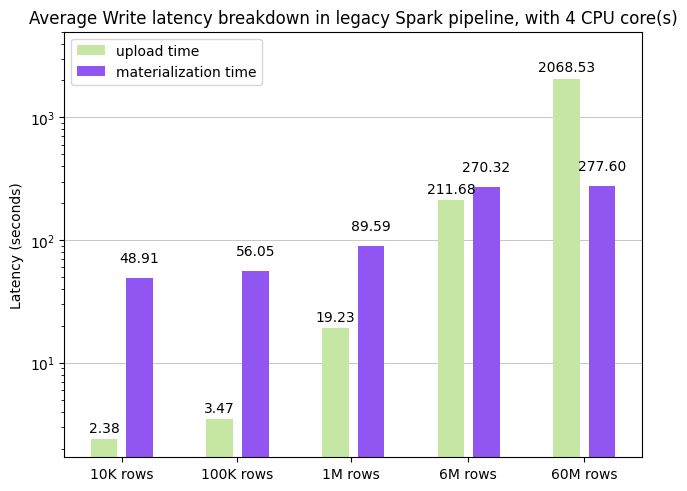
\includegraphics[width=\textwidth]{figures/99-appendix/results-diagrams/write/hudi_upload_materialize/hudi_virtualiz_4_core.png}
        \caption[Histogram of the write on legacy pipeline - Time breakdown - 4 CPU cores]{Histogram in log-scale displaying the contributions to the write latency of the upload and materialization steps in the legacy pipeline. The experiment was performed with four \glstext{CPU} cores.}
        \label{fig:appx_hudi_virtualiz_breakdown_4_core}
    \end{minipage}
\end{figure}

\begin{figure}
    \centering
    \begin{minipage}[b]{\textwidth}
        \centering
        \captionof{table}[Write on legacy pipeline - Time breakdown - 8 cores]{Contributions to the write latency of the upload and materialization steps in the legacy pipeline. The experiment was performed with eight \glstext{CPU} cores.}
        \label{tbl:appx_hudi_virtualiz_breakdown_8_cores}
        \begin{tabular}{l r S[table-format=5.4] S[table-format=5.4] S[table-format=5.4] S[table-format=5.4]} 
            \toprule
            {\multirow{2}{*}{Step\Tstrut\Bstrut}} & \multirow{2}{*}{{\thead{Number\\ of rows}}} & {\multirow{2}{*}{{\thead{Latency \\ (seconds)}}}} & \multicolumn{2}{c}{{\thead{Latency (seconds) \\95\% Confidence Interval}}}\\
                                    &                                             &                                                   & {low} & {high}                                                            \\
            \midrule
            upload                  & \multirow{2}{*}{10K}                        &    2.3815                                         &    2.3304 &    2.4358                                                      \\ 
            materialize             &                                             &   48.8485                                         &   48.1979 &   49.4467                                                      \\
            \midrule
            upload                  & \multirow{2}{*}{100K}                       &    3.4392                                         &    3.4081 &    3.4700                                                      \\                                                                 
            materialize             &                                             &   56.8428                                         &   56.3177 &   57.3685                                                      \\
            \midrule
            upload                  & \multirow{2}{*}{1M}                         &   18.8642                                         &   18.7808 &   18.9532                                                      \\                                                                 
            materialize             &                                             &   90.5153                                         &   90.0306 &   90.9718                                                      \\
            \midrule
            upload                  & \multirow{2}{*}{6M}                         &  207.6646                                         &  207.1606 &  208.2090                                                      \\                                                                 
            materialize             &                                             &  268.2752                                         &  267.3569 &  269.2456                                                      \\
            \midrule
            upload                  & \multirow{2}{*}{60M}                         & 2049.1371                                         & 2043.5991 & 2055.4782                                                      \\                                                                 
            materialize             &                                             &  275.7636                                         &  274.2773 &  274.2773                                                      \\
            \bottomrule
        \end{tabular}
    \end{minipage}
    \begin{minipage}[b]{\textwidth}
        \centering
        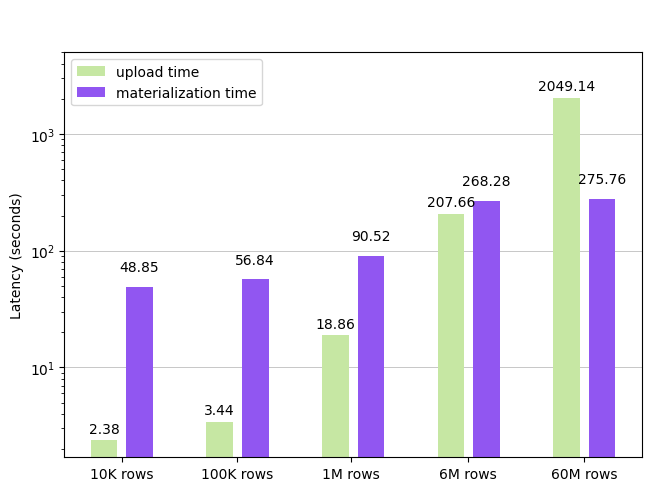
\includegraphics[width=\textwidth]{figures/99-appendix/results-diagrams/write/hudi_upload_materialize/hudi_virtualiz_8_core.png}
        \caption[Histogram of the write on legacy pipeline - Time breakdown - 8 CPU cores]{Histogram in log-scale displaying the contributions to the write latency of the upload and materialization steps in the legacy pipeline. The experiment was performed with eight \glstext{CPU} cores.}
        \label{fig:appx_hudi_virtualiz_breakdown_8_core}
    \end{minipage}
\end{figure}

\cleardoublepage

%% The following label is necessary for computing the last page number of the body of the report to include in the "For DIVA" information
\label{pg:lastPageofMainmatter}

\cleardoublepage

%%%%%%%%%%%%%%%%%%%%%%%%%%%%%%%%%%%%%%%%%%%%%%%%%%%%%%%%%%%%%%%%%%%%%%%%%%%%%%%%%%%%%%%%
%%                                 FOR DIVA MATERIAL
%%%%%%%%%%%%%%%%%%%%%%%%%%%%%%%%%%%%%%%%%%%%%%%%%%%%%%%%%%%%%%%%%%%%%%%%%%%%%%%%%%%%%%%%
\clearpage\thispagestyle{empty}\mbox{} % empty page with backcover on the other side
\kthbackcover
\fancyhead{}  % Do not use header on this extra page or pages
\section*{€€€€ For DIVA €€€€}
\lstset{numbers=none} %% remove any list line numbering
\divainfo{pg:lastPageofPreface}{pg:lastPageofMainmatter}

% If there is an acronyms.tex file,
% add it to the end of the For DIVA information
% so that it can be used with the abstracts
% Note that the option "nolol" stops it from being listed in the List of Listings

% The following bit of ugliness is because of the problems PDFLaTeX has handling a non-breaking hyphen
% unless it is converted to UTF-8 encoding.
% If you do not use such characters in your acronyms, this could be simplified.
\ifxeorlua
\IfFileExists{lib/acronyms.tex}{
\section*{acronyms.tex}
\lstinputlisting[language={[LaTeX]TeX}, nolol, basicstyle=\ttfamily\color{black},
commentstyle=\color{black}, backgroundcolor=\color{white}]{lib/acronyms.tex}
}
{}
\else
\IfFileExists{lib/acronyms-for-pdflatex.tex}{
\section*{acronyms.tex}
\lstinputlisting[language={[LaTeX]TeX}, nolol, basicstyle=\ttfamily\color{black},
commentstyle=\color{black}, backgroundcolor=\color{white}]{lib/acronyms-for-pdflatex.tex}
}
{}
\fi

\end{document}
